%%% Folie
{
\scriptsize

\begin{frame}{Lernziele}
    \begin{columns}
        \begin{column}{.7\textwidth}
            \begin{block}{Linux}
                \begin{itemize}
                    \item Raspberry Pi OS Lite installieren und einrichten können
                    \item Den typischen Aufbau eines Linux-Systems beschreiben können
                    \item Den Bootvorgang von Linux auf des Raspberry Pi erklären können
                    \item Die wichtigsten Verzeichnisse einer Linux-Installation kennen
                    \item Die Benutzer- und Rechteverwaltung von Linux grob verstehen
                \end{itemize}
            \end{block}

            \begin{block}{Python}
                \begin{itemize}
                    \item Eigene Pythonprojekte anlegen und ausprogrammieren können
                    \item Dokumentation und Bibliotheken zur Python online suchen
                    \item Die grundlegenden Eigenheiten von Python beschreiben können
                    \item Einfache Pythonprogramme selbst programmieren können
                    \item Fehler suchen und Pythonprogramme im Debugger testen können
                    \item Größere Programme mit Klassen und Objekten strukturieren können
                \end{itemize}
            \end{block}
        \end{column}

        \begin{column}{.3\textwidth}
            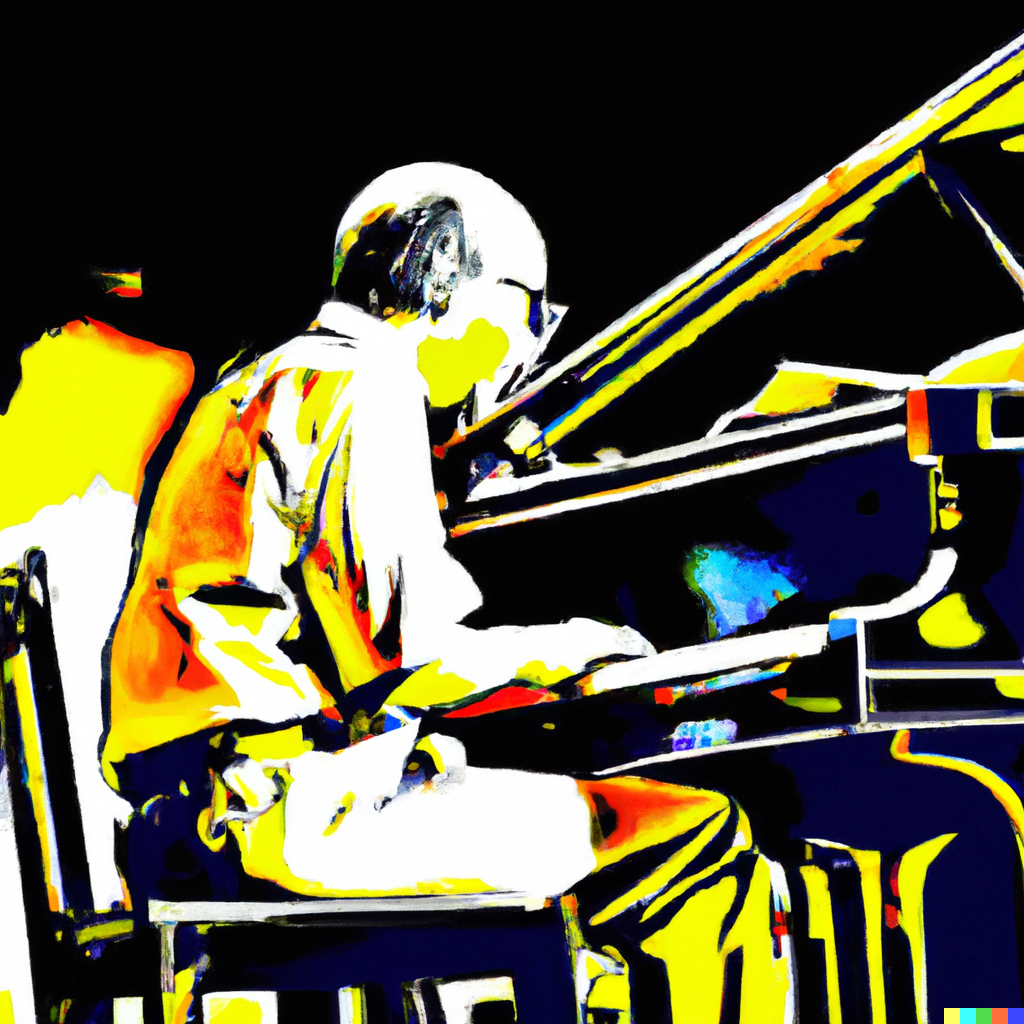
\includegraphics[width=\textwidth]{img/lernziele1}
            
\includegraphics[width=\textwidth]{img/lernziele2}
        \end{column}
    \end{columns}
\end{frame}
}

%-------------------------------------------------------------------------------
\section{Linux auf dem Raspberry Pi}
%-------------------------------------------------------------------------------

%%% Folie
{
\scriptsize

\begin{frame}{Beispiele für Linux-basierte Betriebssysteme}
    \Justified{
        Ursprünglich vom finnischen Informatikstudenten Linux Torvalds als Hobbyprojekt
        geschrieben, läuft Linux heute auf nahezu jeder Hardware. Dabei bezeichnet der
        Name ,,Linux'' allerdings nur den Kernel, der die Grundlage für viele Betriebssysteme
        (Linux-Distributionen) auf den unterschiedlichsten Computersystemen bildet.
        \medskip
    }

    
\includegraphics[width=\textwidth]{img/linux-beispiele}
\end{frame}
}

%%% Folie
{
\scriptsize

\begin{frame}{Über das Raspberry Pi OS}
    \Justified{
        Für den Raspberry Pi werden inzwischen viele verschiedene Linux-Distributionen
        angeboten. Am häufigsten wird jedoch das \textbf{Raspberry Pi OS} der Raspberry Pi
        Foundation (basierend auf Rasbpian bzw. Debian) verwendet, da es oftmals schon
        vorinstalliert mitgeliefert wird. Dabei handelt es sich allerdings nicht primär
        um ein Betriebssystem für eingebettete Awendungen, sondern um ein ausgewachsenes
        Desktop-Betriebssystem.
        \smallskip

        Denn ursprünglich wurde der Raspberry Pi, wie viele Computer vor ihm, in Großbritanien
        als kostengünstiges Lern- und Experimentiergerät für Kinder und Jugendliche entworfen.
        In der Vorlesung verwenden wir daher die Lite-Version des Raspberry Pi OS, da diese
        einem minimalen Linux-Grundsystem entspricht.
    }

    \medskip

    \begin{columns}[b,onlytextwidth]
        \column{.48\textwidth}
        \begin{center}
            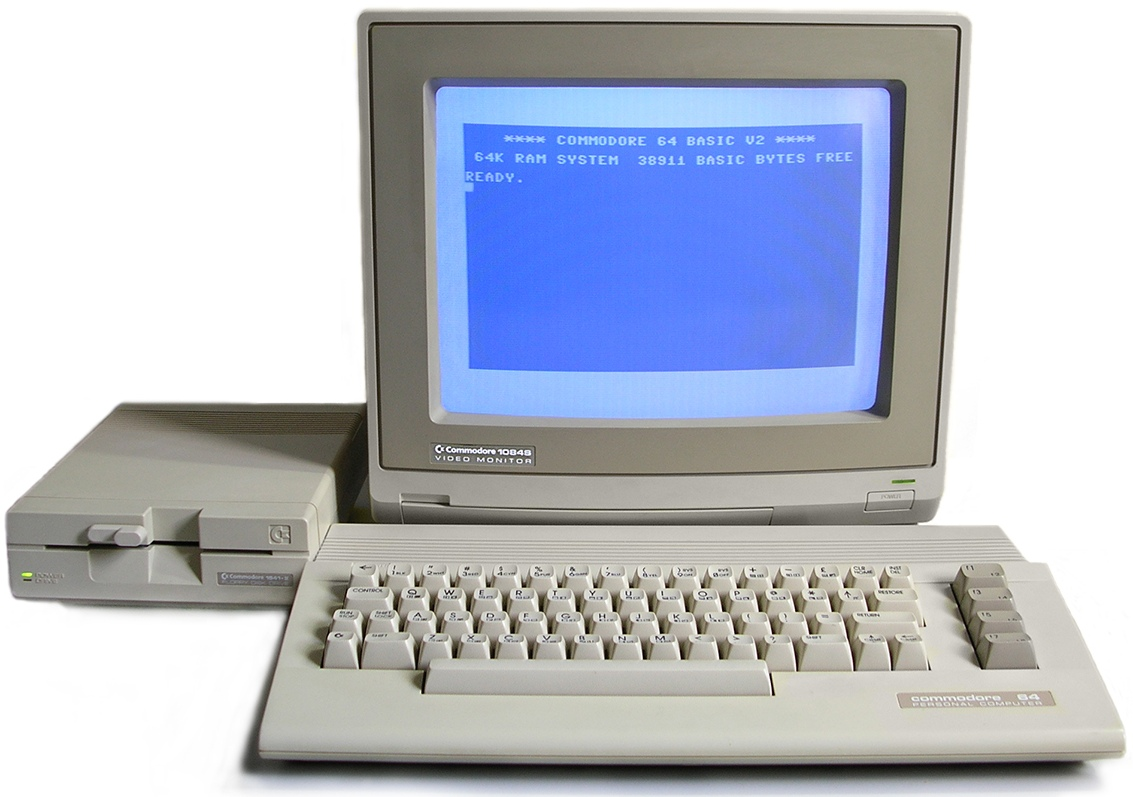
\includegraphics[width=.9\textwidth]{img/c64}
        \end{center}
        \Justified{
            \textbf{Commodore 64:}
            Früher Heimcomputer der 1980er-Jahre
            mit eingebautem BASIC-Interpreter
        }

        \column{.48\textwidth}
        \begin{center}
            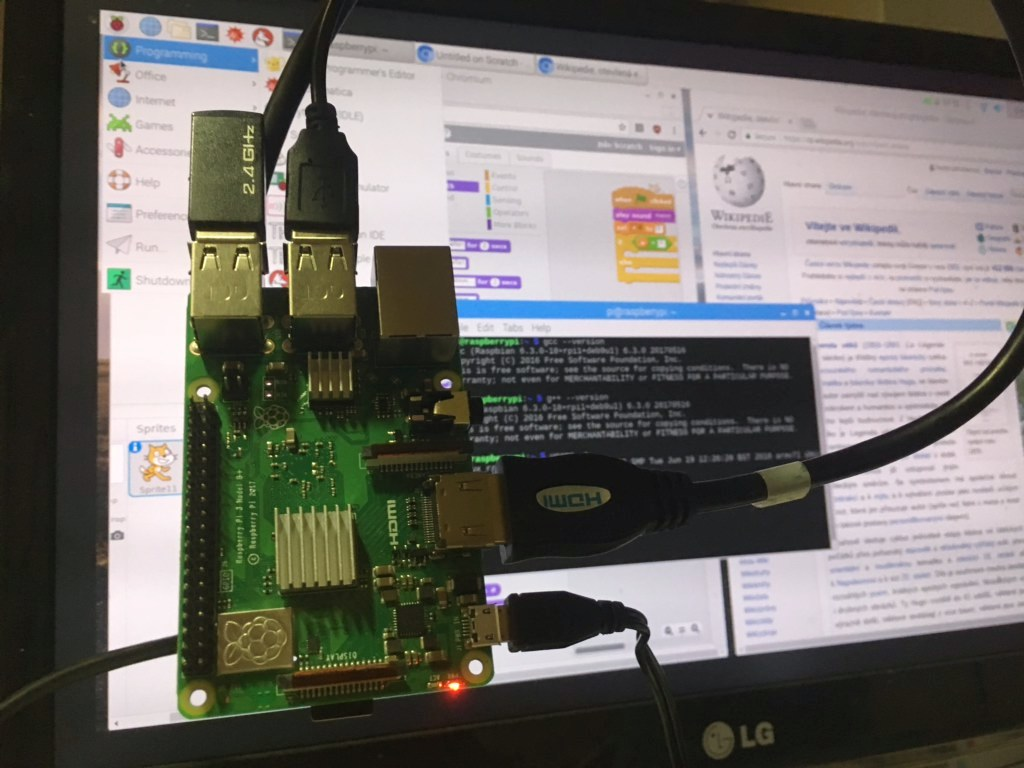
\includegraphics[width=.85\textwidth]{img/raspi}
        \end{center}
        \Justified{
            \textbf{Rasbperry Pi:} Moderner Versuch, einen Computer zum
            Experimentieren und Programmieren Lernen zu bauen
        }
    \end{columns}
\end{frame}
}

%%% Folien
{
\scriptsize
\setlength{\fboxsep}{0pt}

\begin{frame}[allowframebreaks]{Installation des Raspberry Pi OS}
    \begin{center}
        \fbox{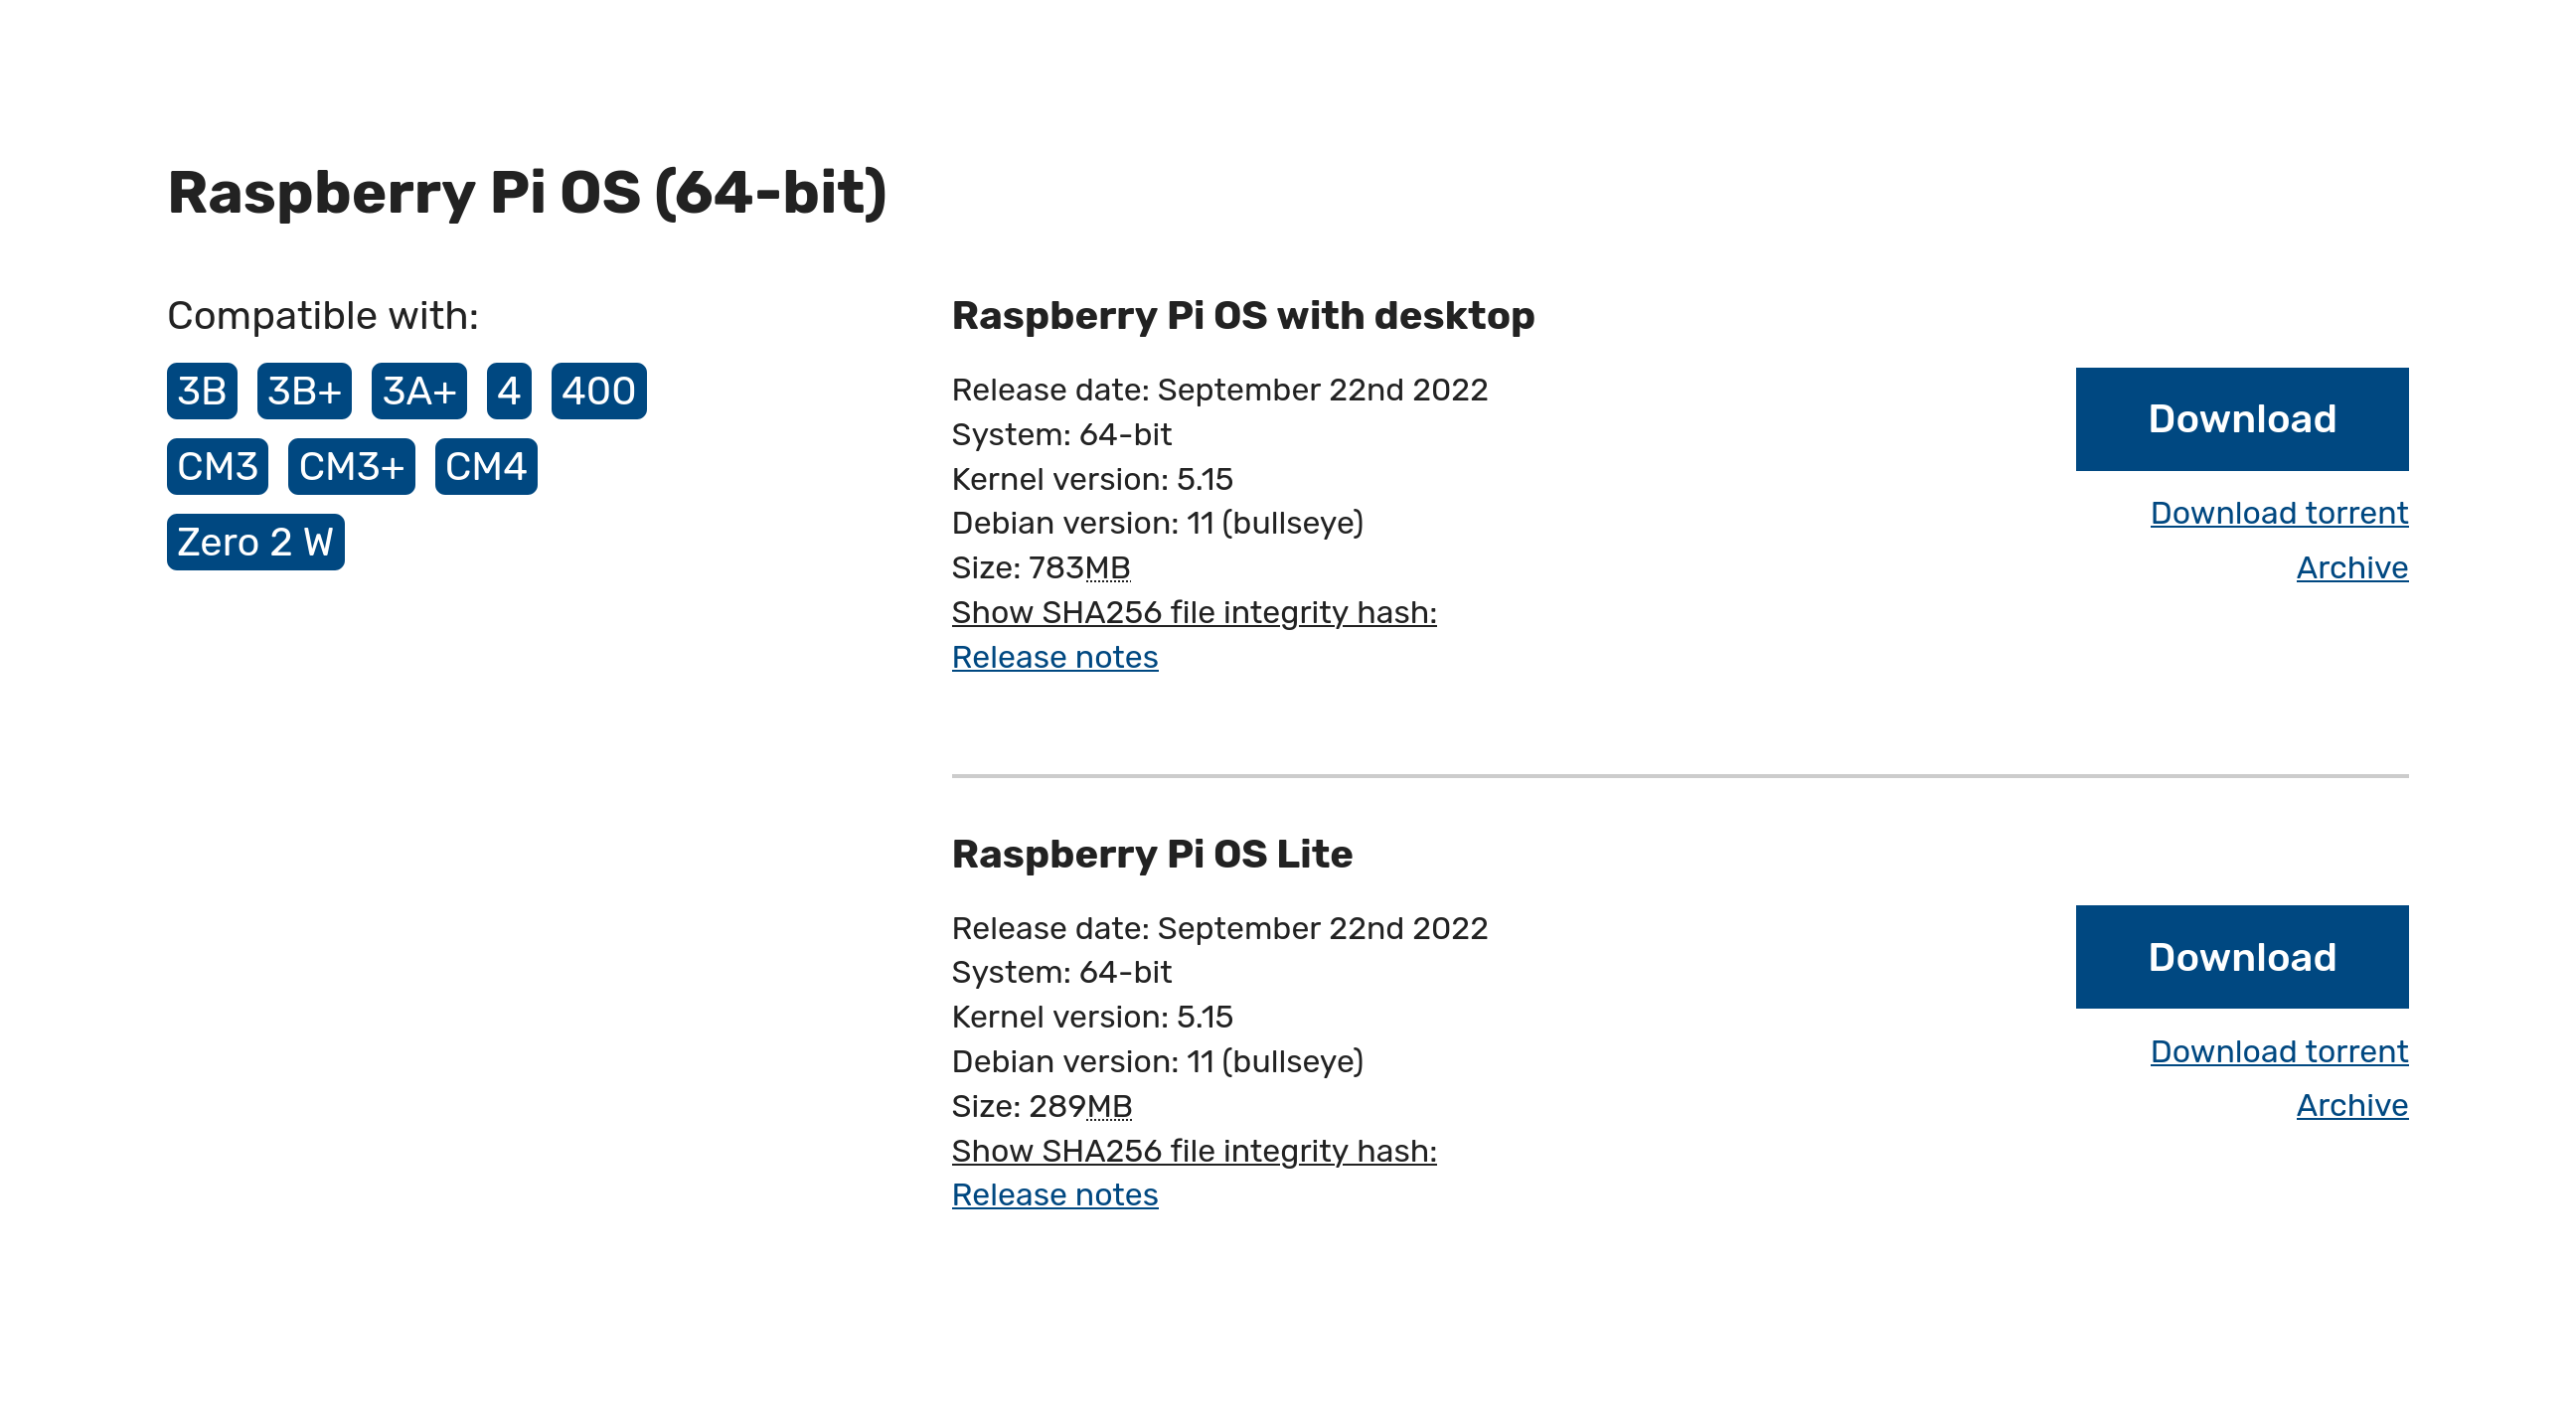
\includegraphics[width=.9\textwidth]{img/raspios-download}}
    \end{center}

    \Justified{
        Das Rasbperry Pi OS (abgeleitet von Raspbian bzw. Debian Linux) wird als Image File
        auf der offiziellen Webseite der Rasbperry Pi Foundation zum Download angeboten.
        Für eingebettete Anwendungen sollte bevorzugt die Lite-Variante ohne Desktopumgebung
        und Anwendungssoftware verwendet werden. Mit entsprechendem Expertenwissen kann man
        natürlich auch sein eigenes Linux-System bauen, zum Beispiel mit Buildroot. \smiley{}
    }

    \smallskip
    \LinkButton{https://www.raspberrypi.com/software/operating-systems/}{Downloadseite des Raspberry Pi OS}
    \LinkButton{https://www.wpvs.de/repo/iot-workshop/05-Werkzeuge/Erste\%20Schritte\%20mit\%20Linux,\%20Buildroot\%20und\%20Debootstrap.pdf}{Anleitung zum Selberbauen}

    %%%
    \framebreak

    \begin{center}
        \fbox{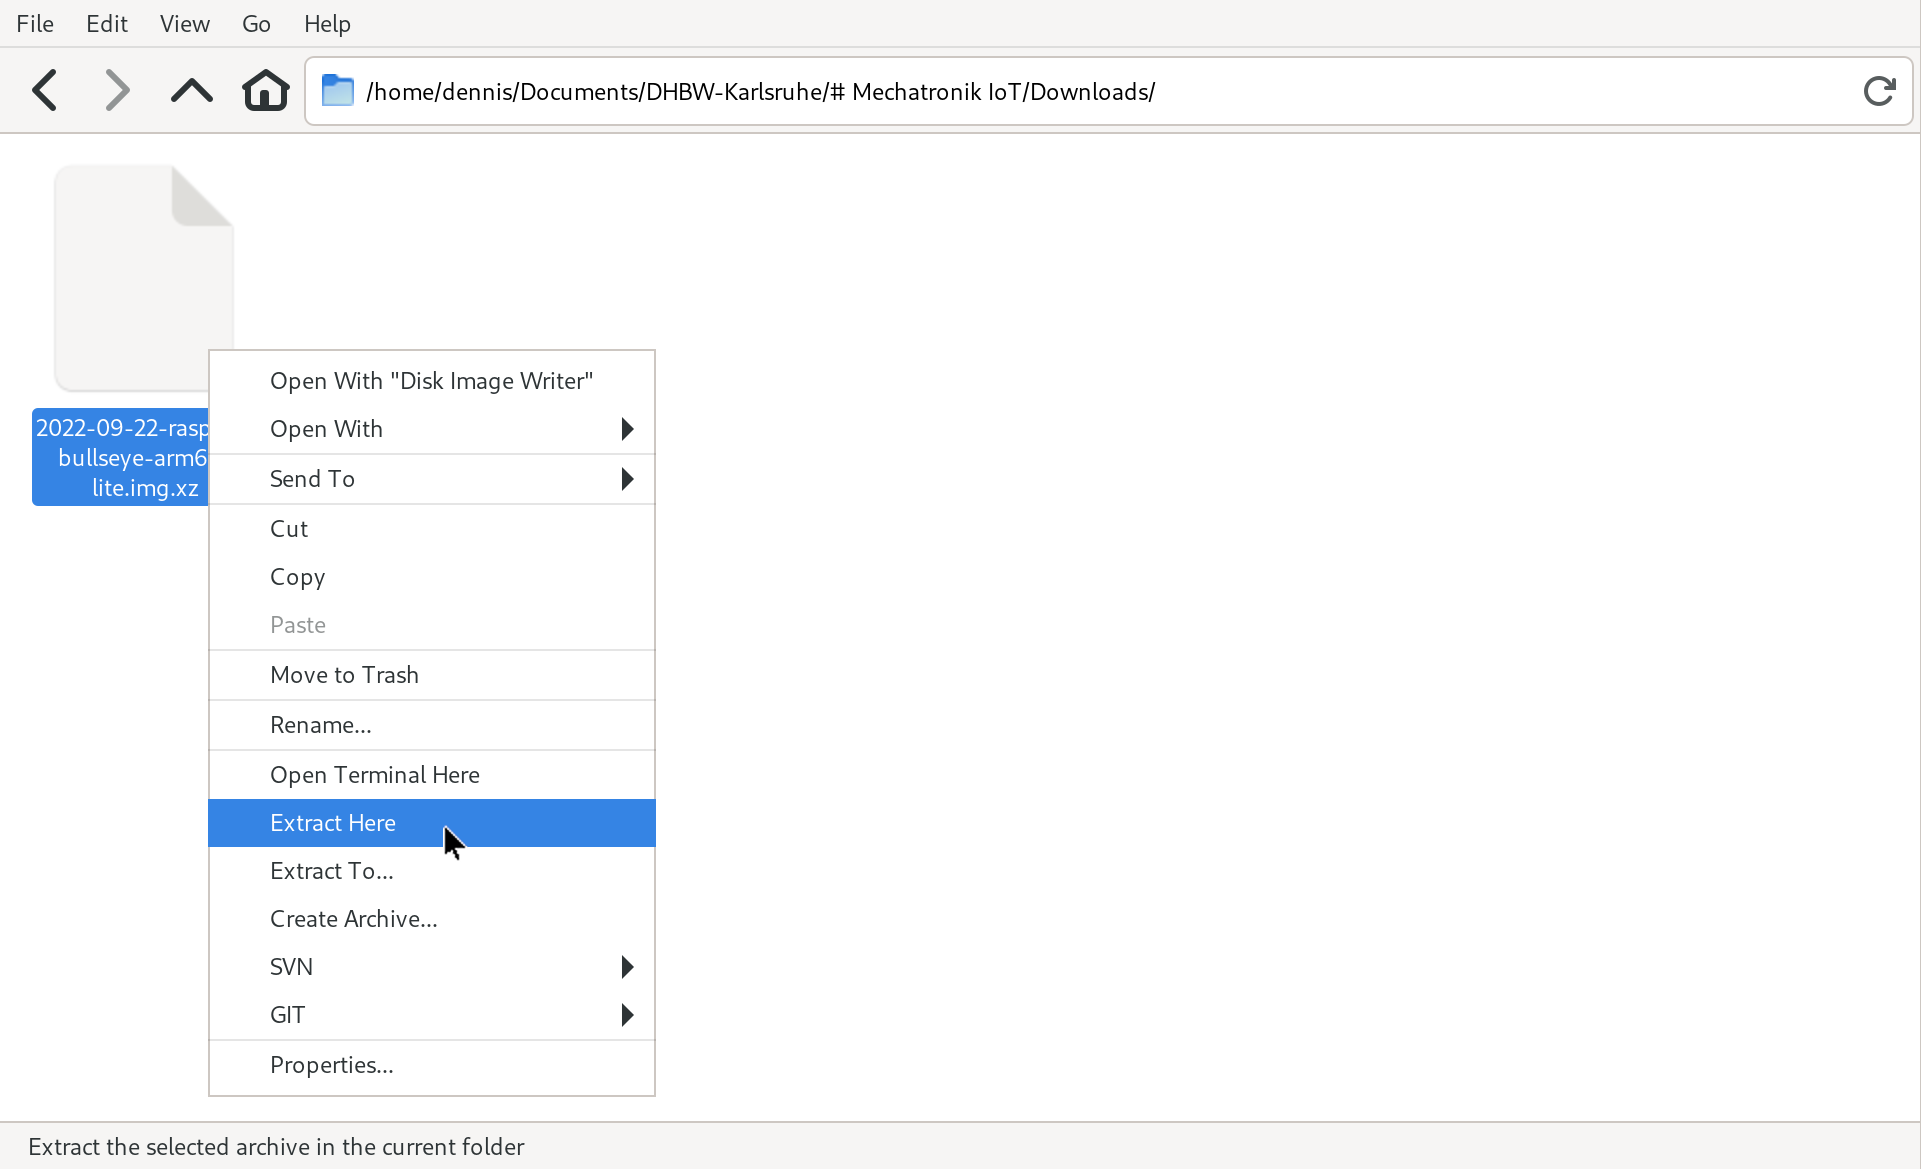
\includegraphics[width=.9\textwidth]{img/raspios-entpacken}}
    \end{center}

    \Justified{
        Um die Downloadgröße klein zu halten, ist die Abbilddatei komprimiert. Sie muss daher mit
        einem geeigneten Programm zunächst entpackt werden, wenn das Programm zum Schreiben der
        SD-Karte dies nicht automatisch macht.
    }

    %%%
    \framebreak

    \begin{center}
        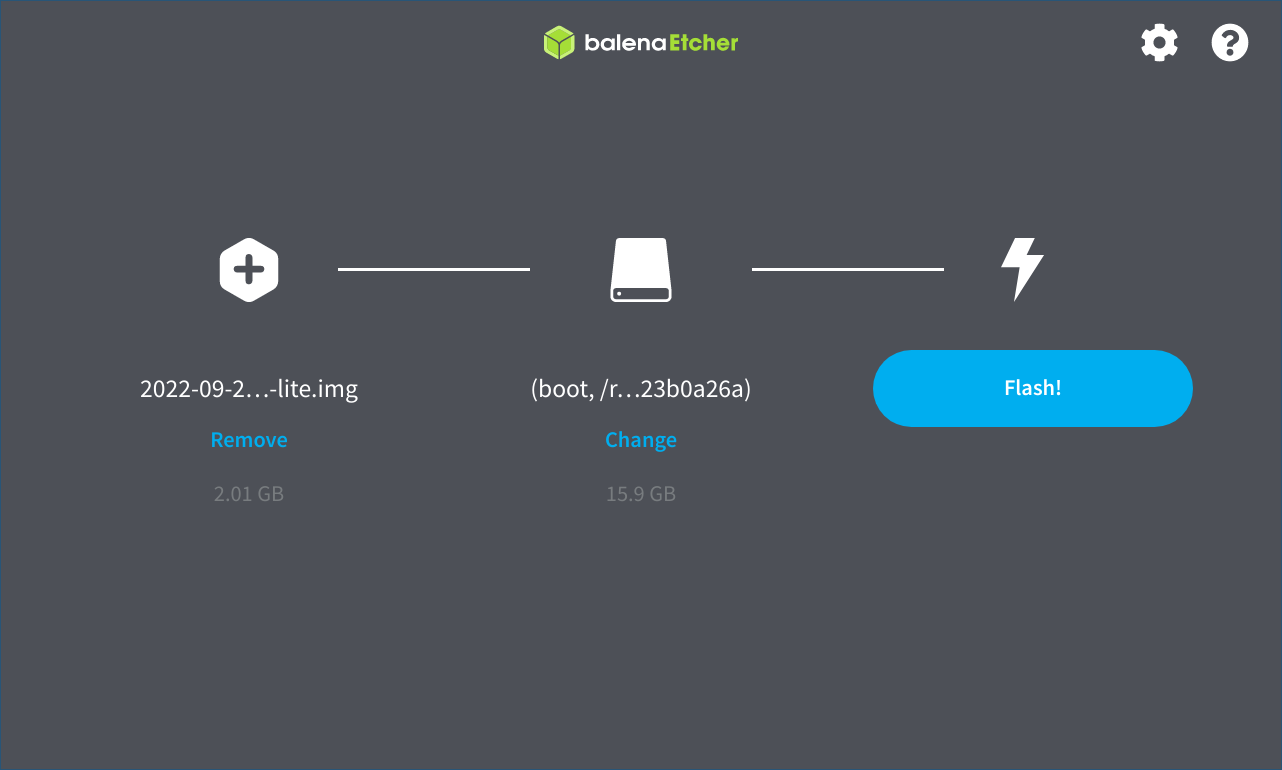
\includegraphics[width=.75\textwidth]{img/raspios-flash}
    \end{center}

    \Justified{
        Anschließend kann die Datei mit einem geeigneten Programm auf eine SD-Karte geschrieben werden.
        Wichtig ist, dass \textcolor{RoyalPurple}{der Inhalt der Datei bitweise} übertragen wird.
        Hierfür kann zum Beispiel der Balena Etcher, der für alle gängigen Betriebssysteme zur Verfügung
        steht, verwendet werden. Ein einfaches Kopieren der Datei mit dem Explorer wird hingegen nicht
        funktionieren.
    }

    \smallskip
    \LinkButton{https://www.balena.io/etcher/}{Downloadseite des Balena Etcher}

    %%%
    \framebreak

    \begin{center}
        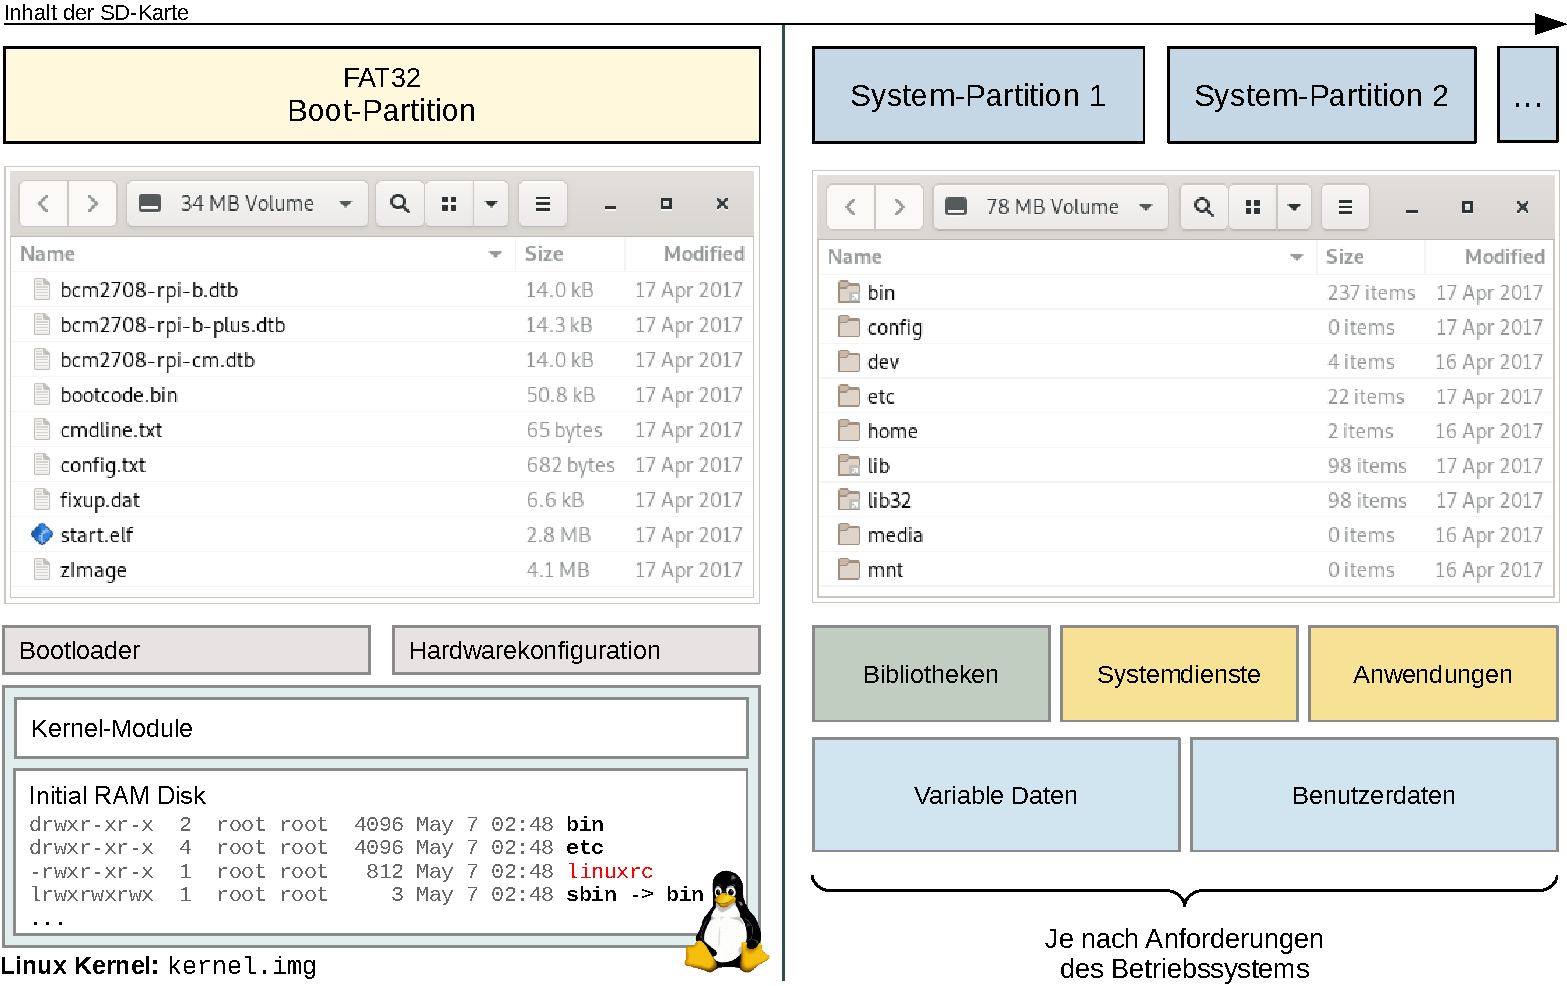
\includegraphics[width=.9\textwidth]{img/raspios-partitionen}
    \end{center}

    \Justified{
        Im Ergebnis sollten mindestens zwei Partitionen auf der SD-Karte vorhanden sein, wobei unter
        Windows nur die Boot-Partition angezeigt wird. Vom Linux-Kernel abgesehen liegen das eigentliche
        Betriebssystem sowie alle Anwendungsdaten in der zweiten Partition.
    }
\end{frame}
}

%%% Folie
\begin{frame}{Der Bootvorgang des Raspberry Pi im Detail}
    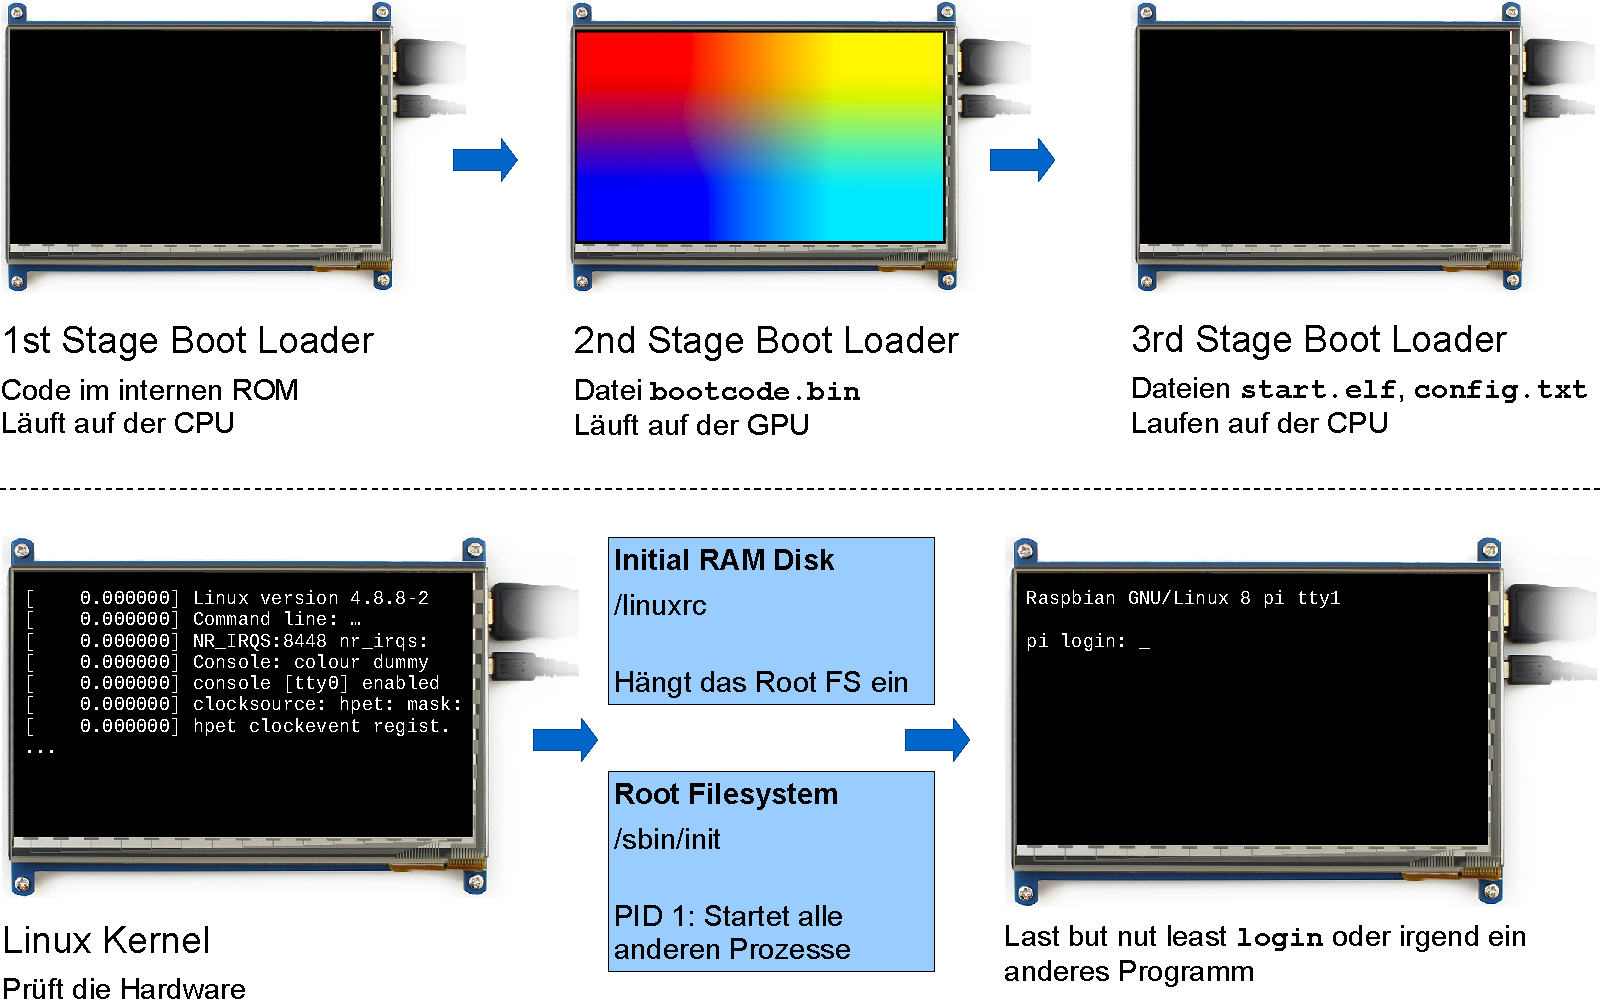
\includegraphics[width=\textwidth]{img/pi-bootvorgang}
\end{frame}

%%% Folien
{
\scriptsize
\setlength{\fboxsep}{0pt}

\begin{frame}[allowframebreaks]{Abschluss der Installation}
    \begin{center}
        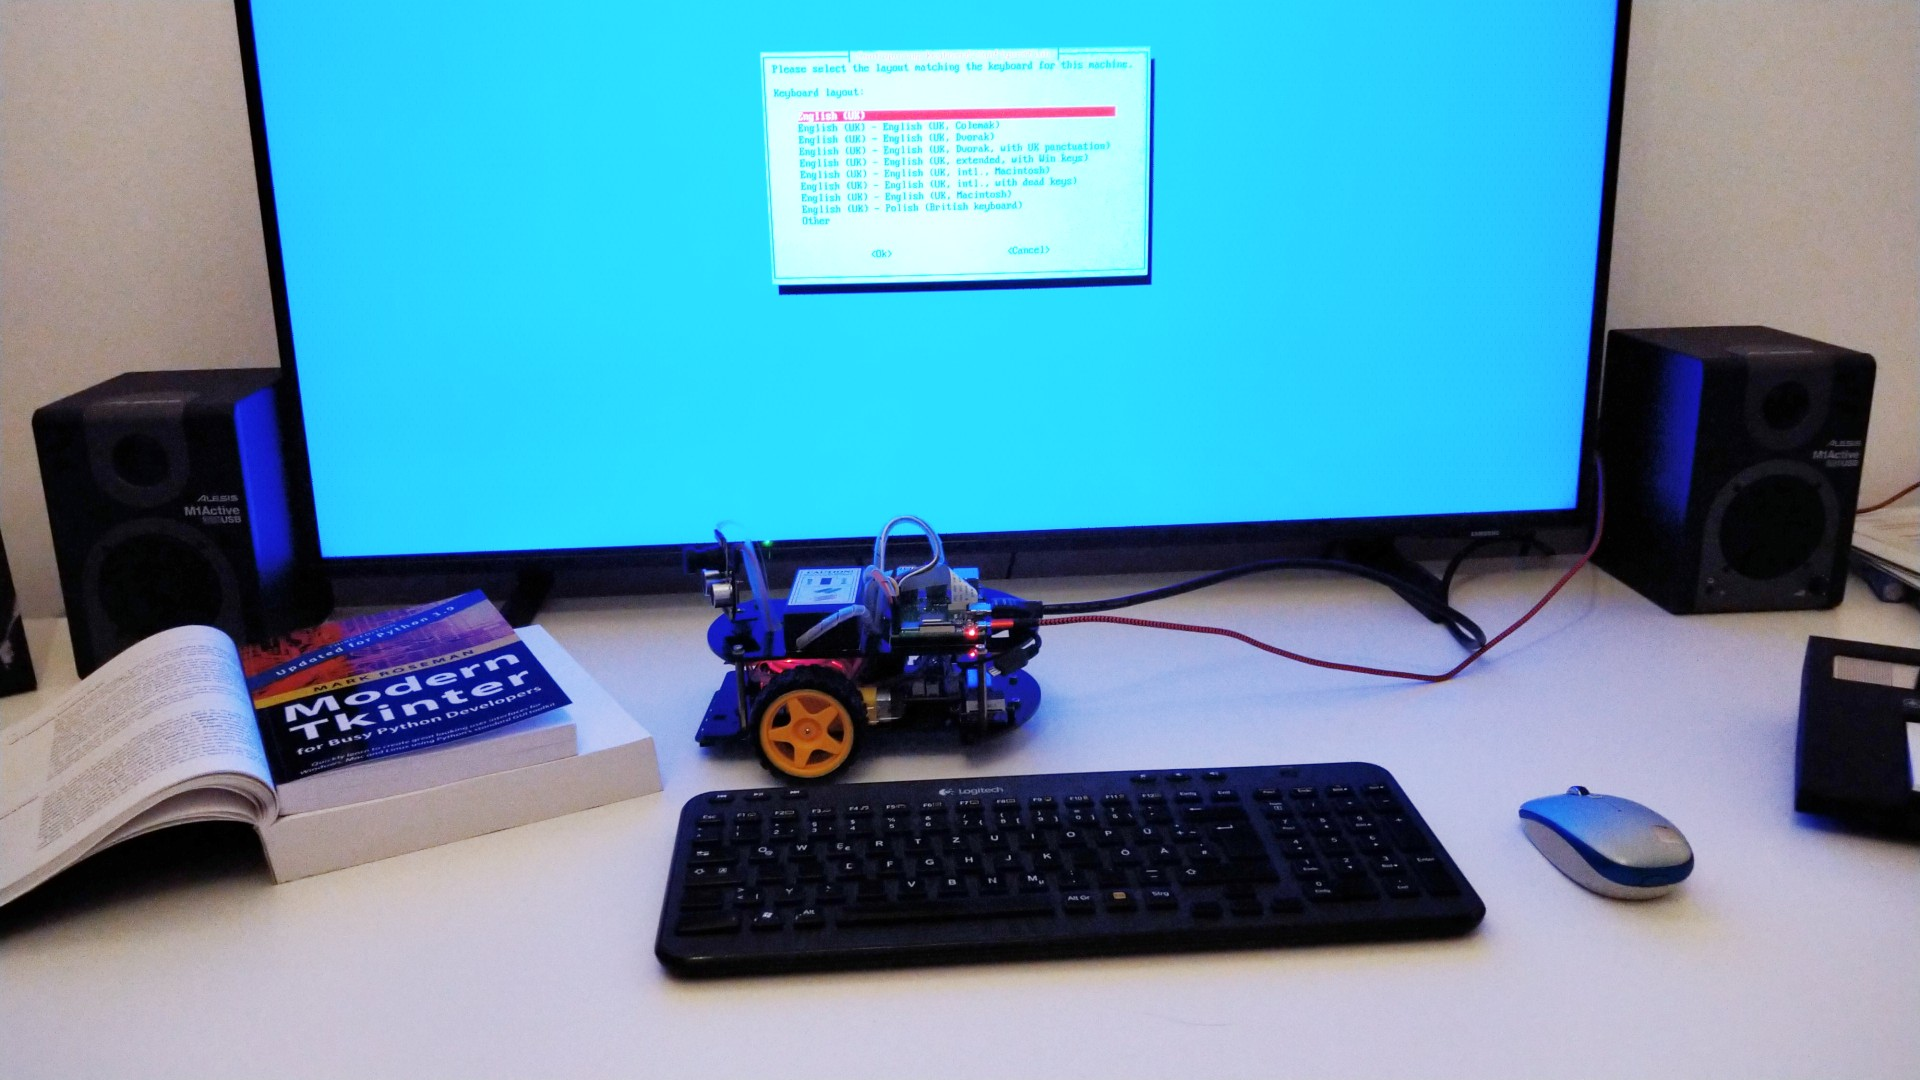
\includegraphics[width=.9\textwidth]{img/raspios-erststart}
    \end{center}

    \Justified{
        Die nächsten Schritte erfolgen auf dem Raspberry Pi. Hierfür müssen zumindest einmal
        Bildschirm, Tastatur und Maus verbunden werden. Anschließend die SD-Karte einlegen und das
        USB-Stromkabel einstecken. Nach einer Weile sollte das System neustarten und ein Menü zum
        Abschluss der Installtion zeigen.
    }

    %%%
    \framebreak

    \begin{center}
        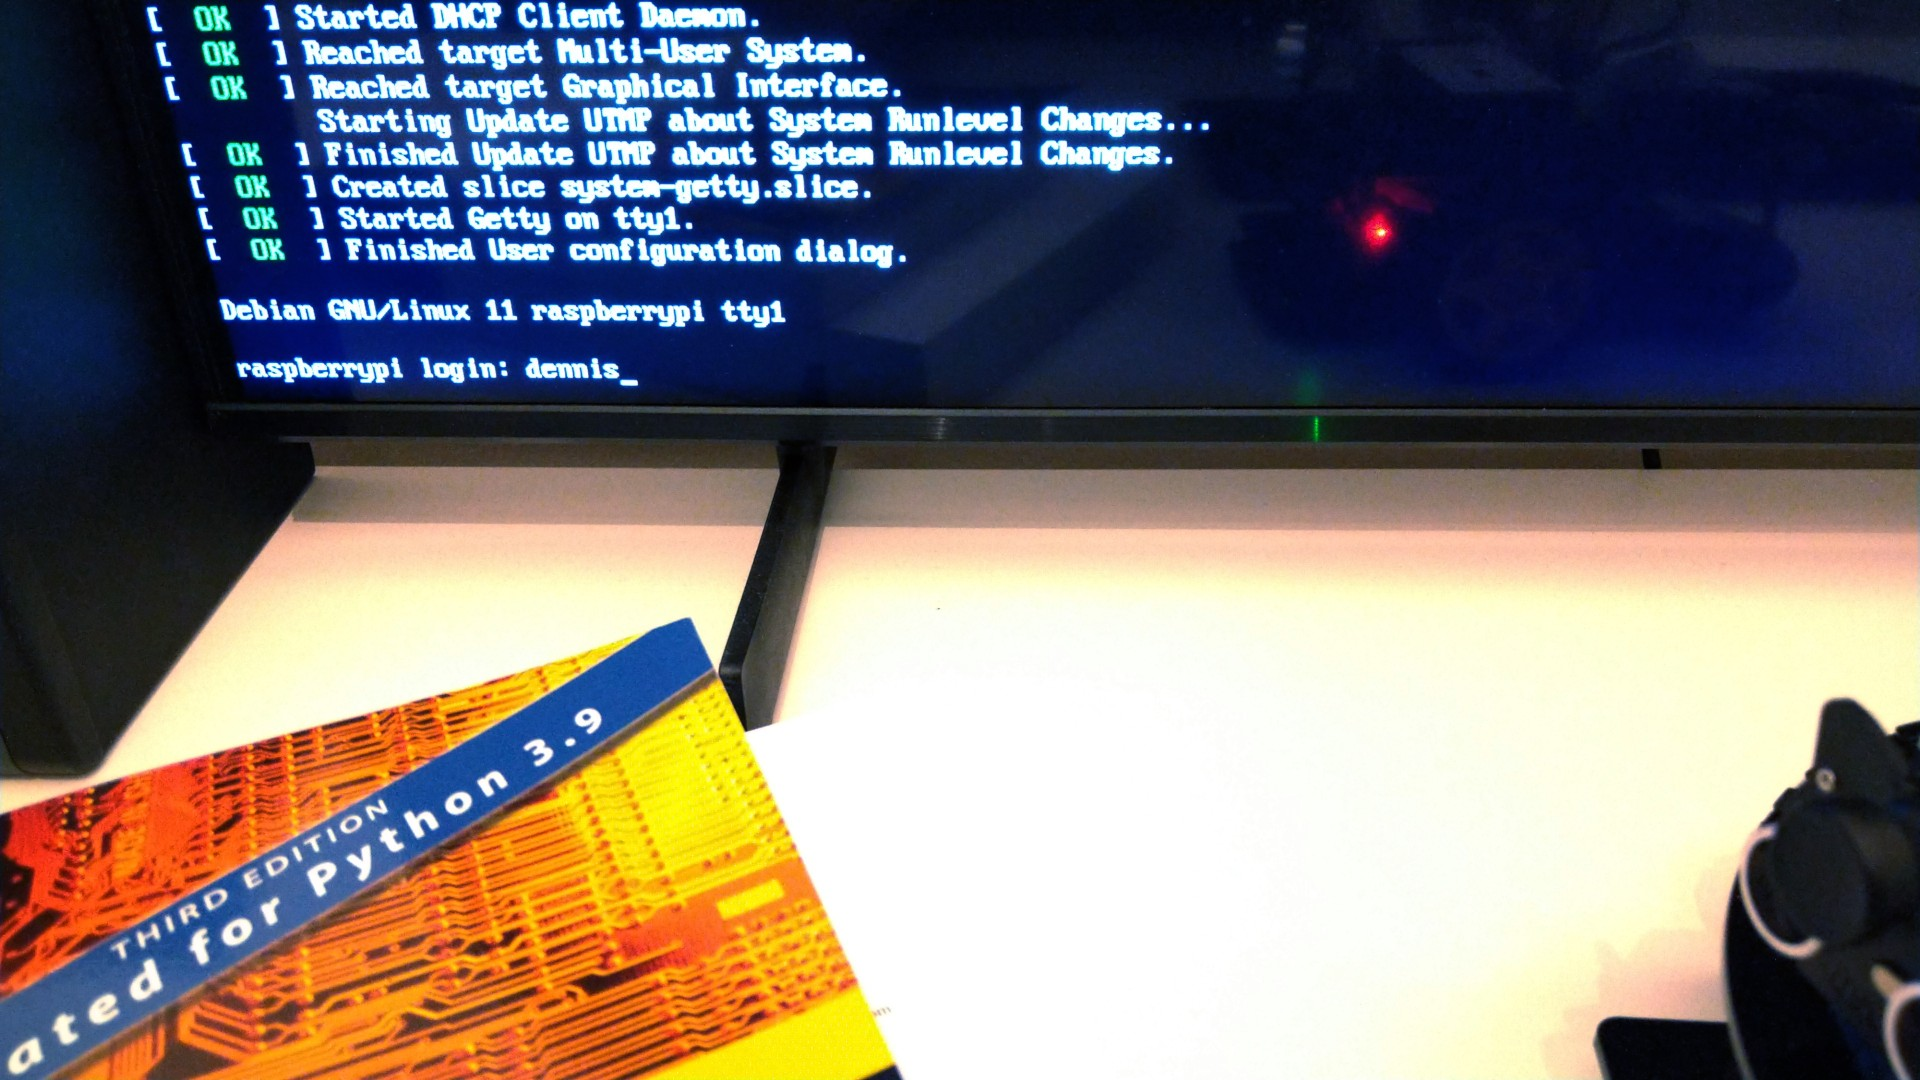
\includegraphics[height=14em]{img/raspios-login}
        \hfill
        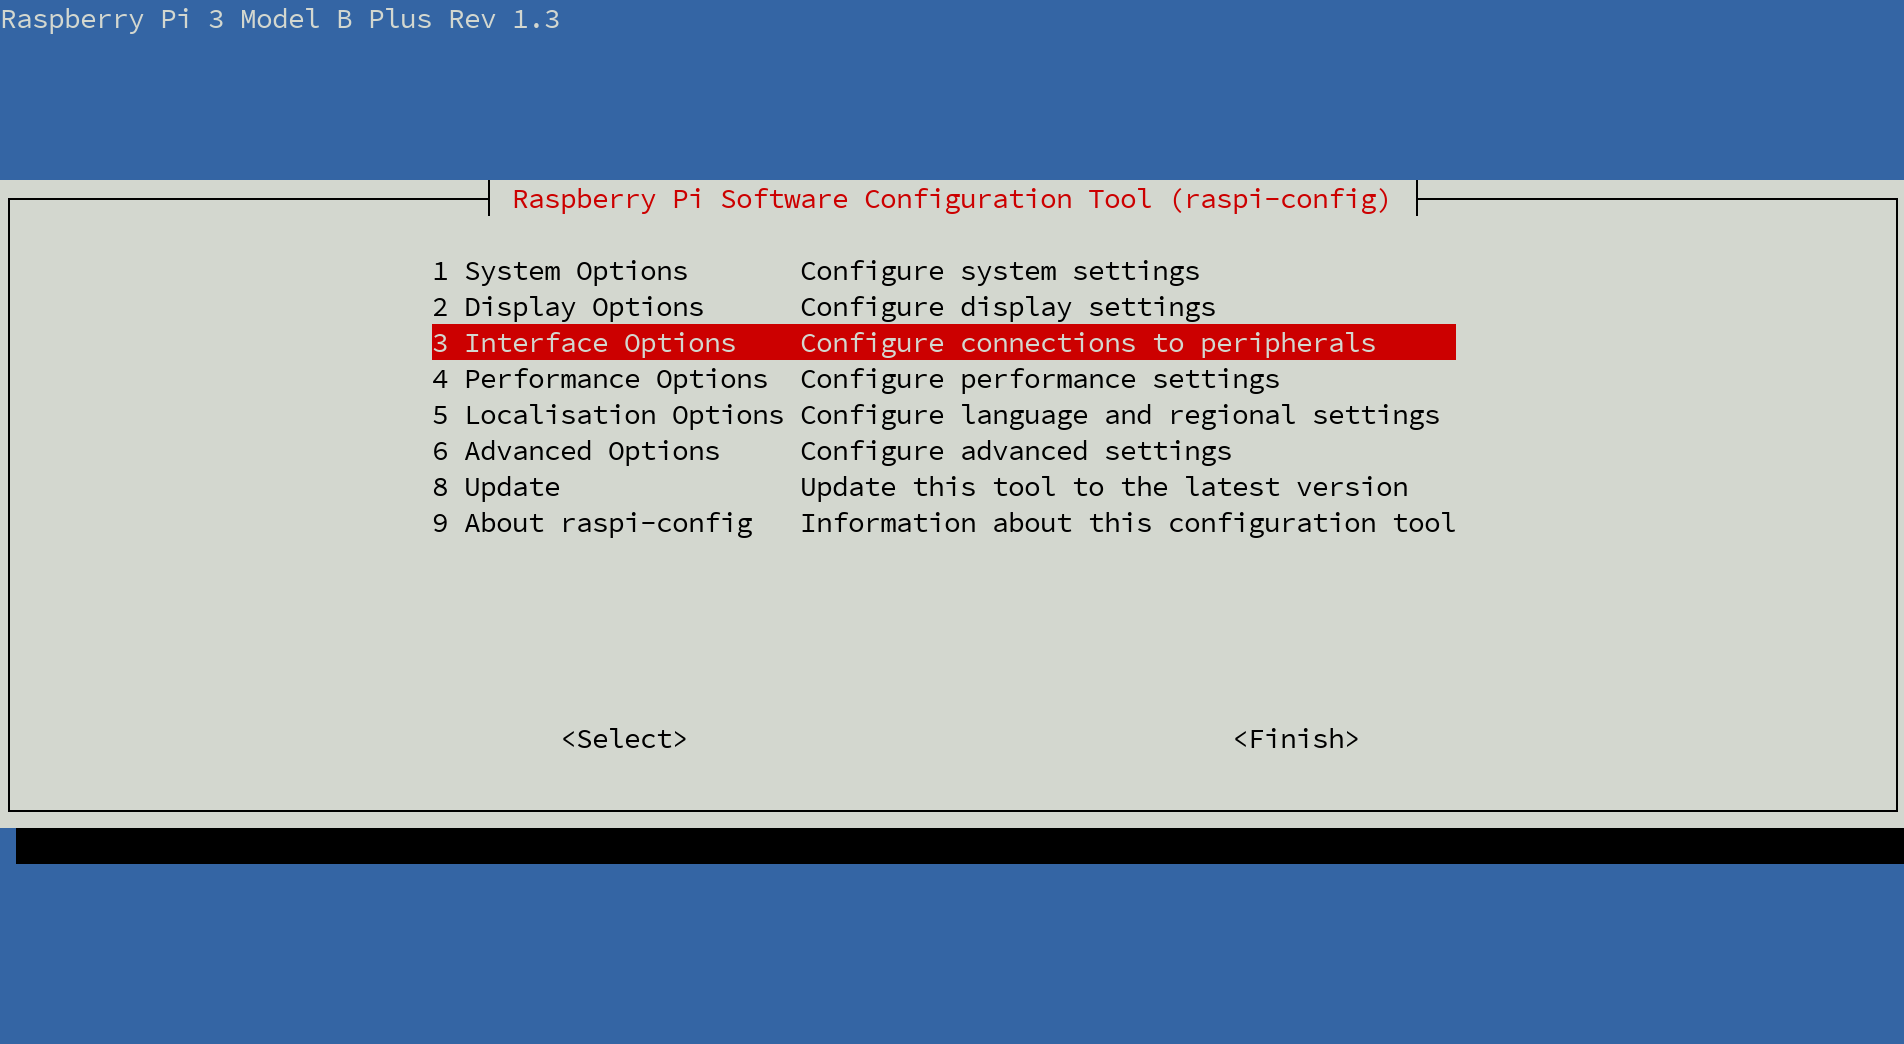
\includegraphics[height=14em]{img/raspi-config-1}
    \end{center}

    %~ \begin{center}
        %~ 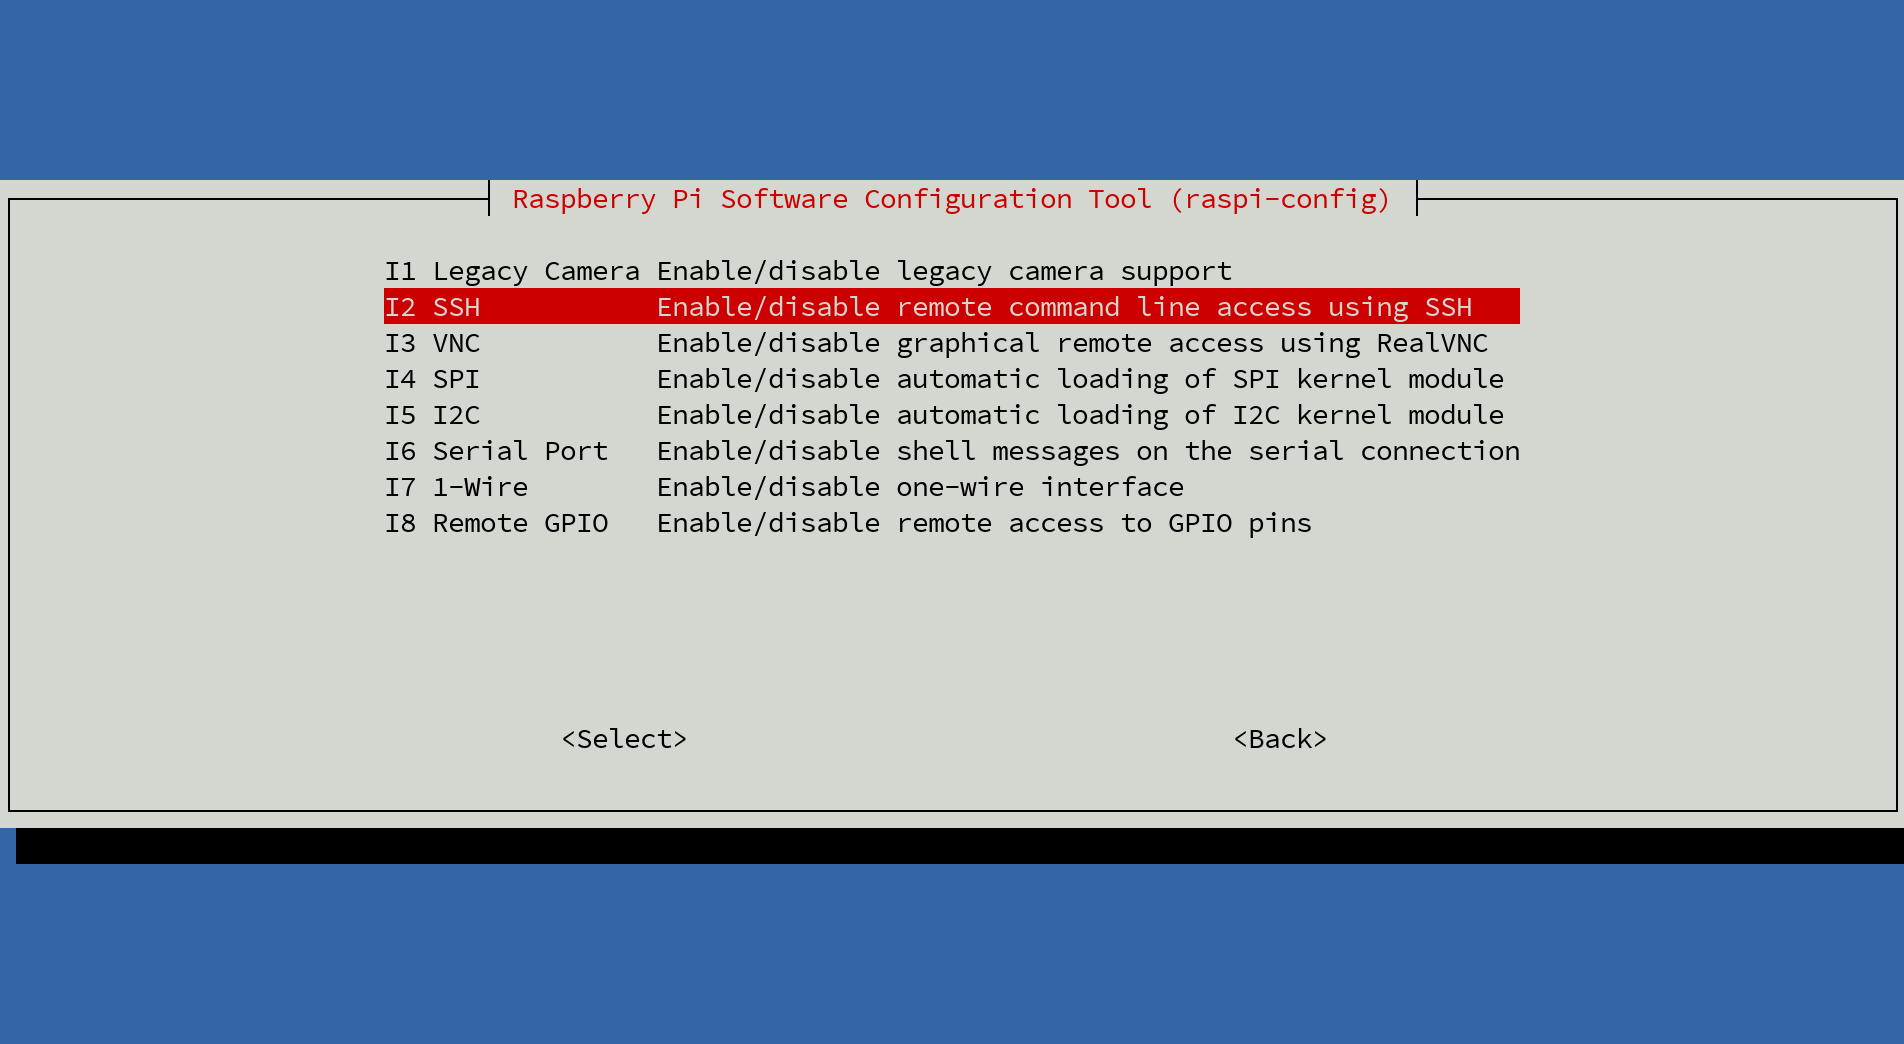
\includegraphics[height=14em]{img/raspi-config-2}
        %~ \hfill
        %~ 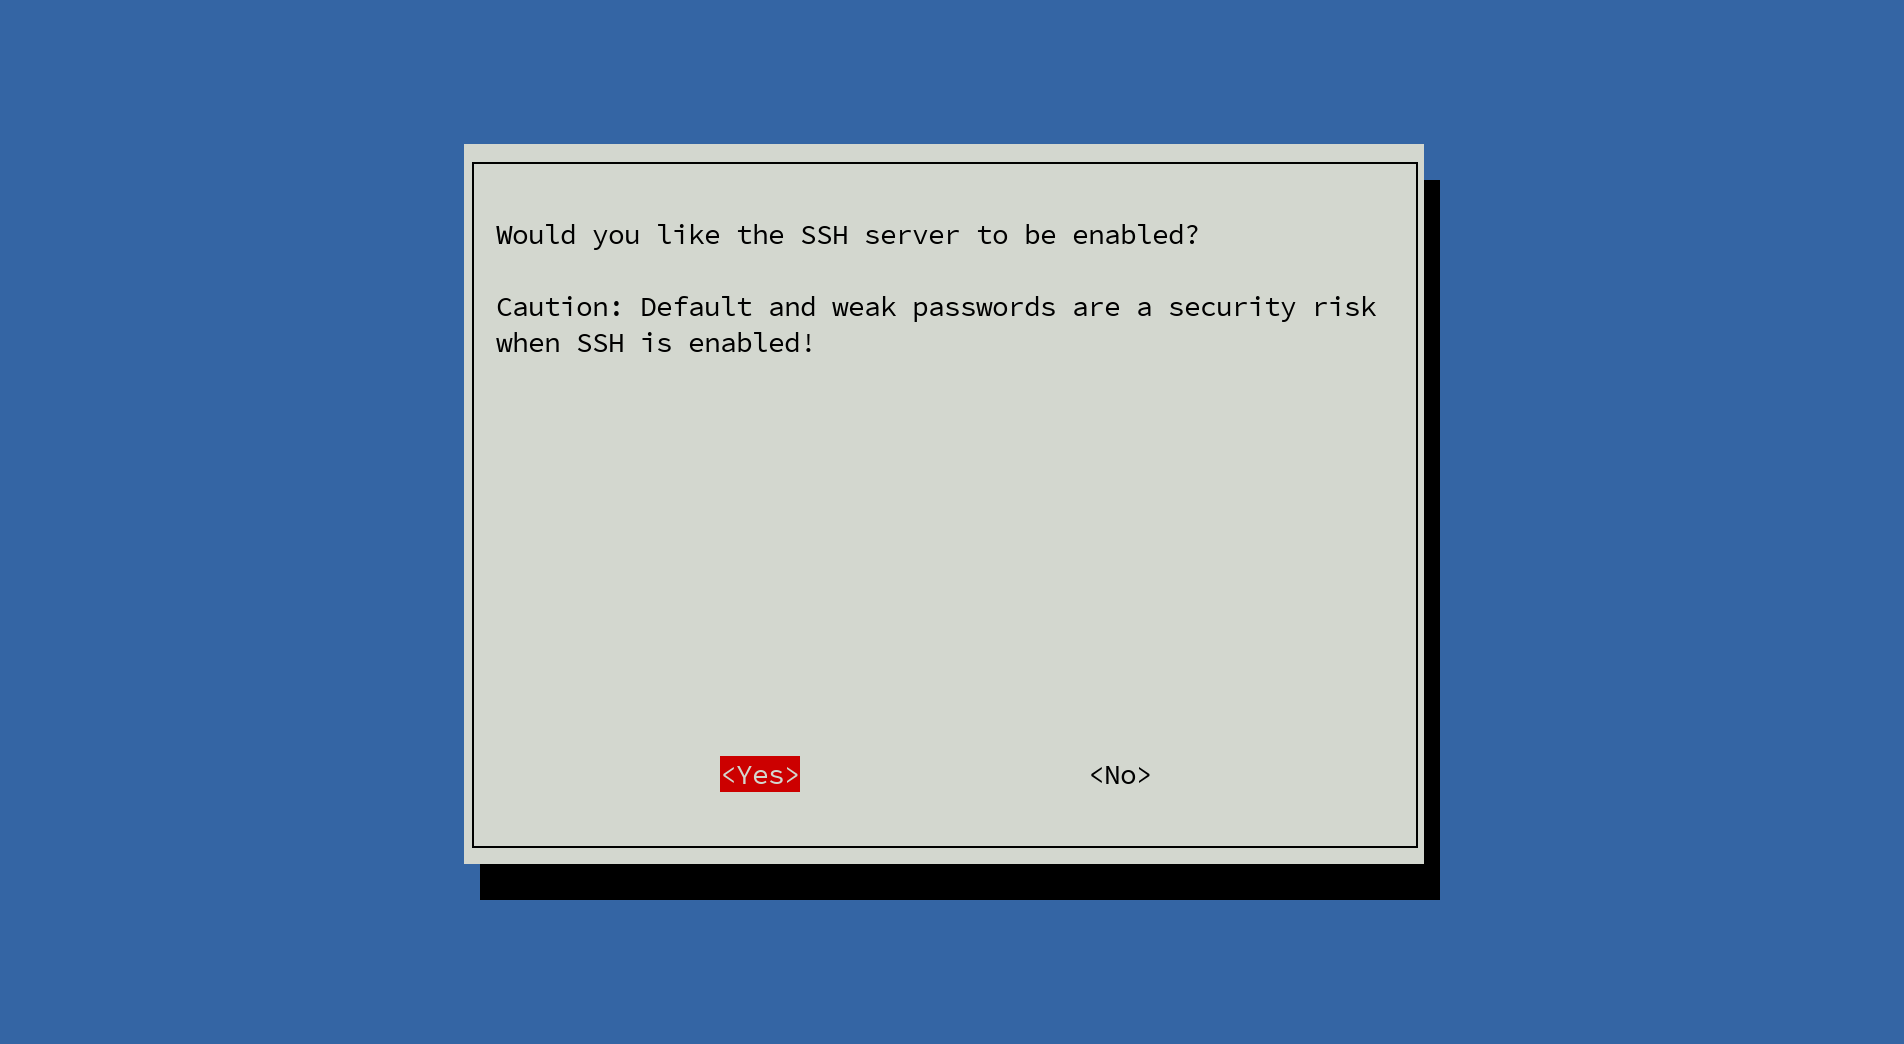
\includegraphics[height=14em]{img/raspi-config-3}
    %~ \end{center}

    \Justified{
        \smallskip
        Kurz darauf erscheint der Login-Prompt. Dort Benutzernamen und Passwort eingeben, um sich
        anzumelden und dann den Befehl \texttt{sudo raspi-config} ausführen. Es handelt sich dabei
        um ein einfaches Konfigurationswerkzeug für das Raspberry Pi OS. Folgende Einstellungen sind
        dort für uns relevant:
        \smallskip
    }

    \begin{itemize}
        \item System Options $\rightarrow$ Wireless LAN $\rightarrow$ \textit{Name und Passwort des WLANs}
        \item Interface Options $\rightarrow$ SSH $\rightarrow$ \textit{aktivieren}
        \item Interface Options $\rightarrow$ SPI $\rightarrow$ \textit{aktivieren}
        \item Interface Options $\rightarrow$ I2C $\rightarrow$ \textit{aktivieren}
        \item Interface Options $\rightarrow$ 1-Wire $\rightarrow$ \textit{aktivieren}
    \end{itemize}

    \Justified{
        \smallskip
        Anschließend muss der Raspberry Pi neugestartet werden, um die Änderungen wirksam werden zu lassen.
    }

    %%%
    \framebreak

    \begin{center}
        \fbox{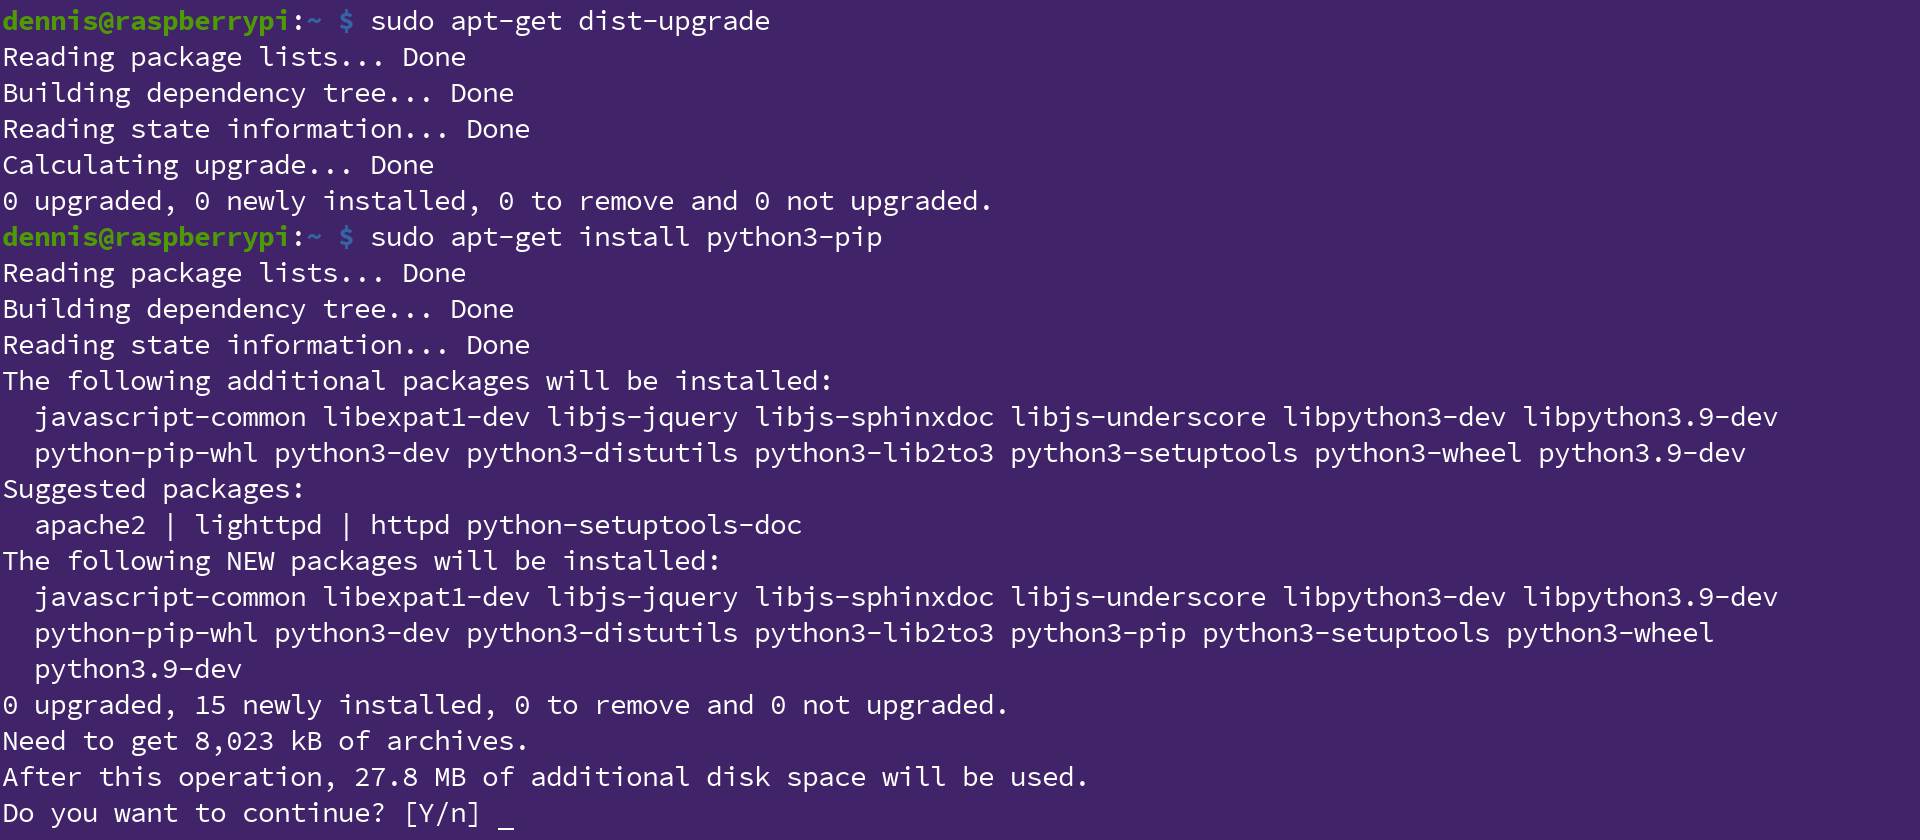
\includegraphics[width=\textwidth]{img/raspios-apt}}
    \end{center}

    \Justified{
        Zum Schluss führen Sie noch folgende Befehle aus, um eventuell vorhandene Update einzuspielen,
        sowie zusätzliche Programme zu installieren:
        \smallskip

        \texttt{sudo apt dist-upgrade} \\
        \texttt{sudo apt install python3-pip python3-venv git golang}
    }
\end{frame}
}

%%% Folie
\begin{frame}{Der Alltag mit Linux \smiley{}}
    \begin{center}
        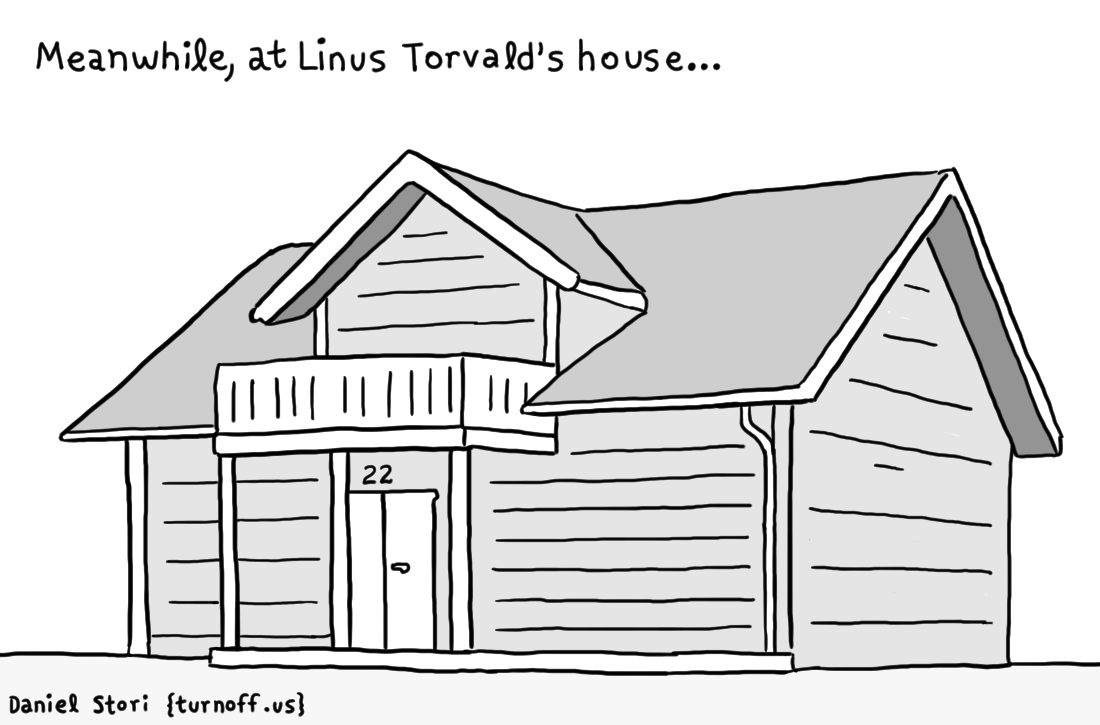
\includegraphics[width=.7\textwidth]{img/linus-torvalds-house}
    \end{center}

    \smallskip

    \begin{center}
        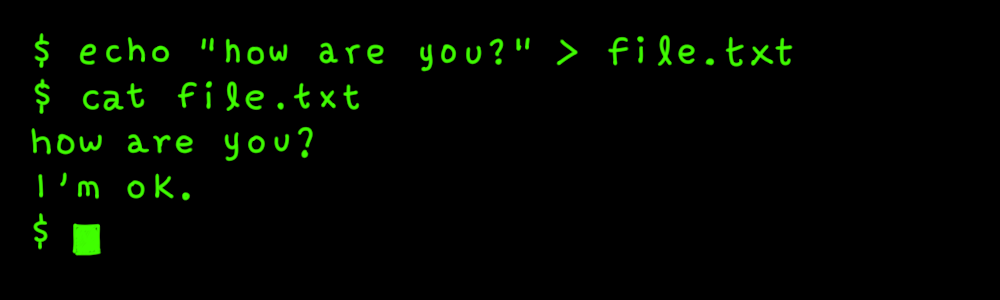
\includegraphics[width=.7\textwidth]{img/ghost-in-the-shell}
    \end{center}
\end{frame}

%%% Folie
{
\scriptsize
\setlength{\leftmargini}{1.2em}

\begin{frame}{Kernel vs. Userland}
    \Justified{
        Linux-basierte Betriebssysteme setzen sich immer aus dem \textbf{Kernel}
        und dem \textbf{Userland} zusammen. Der Kernel beinhaltet dabei lediglich
        die Grundfunktionen für Hardwarezugriffe, Multitasking, Speicherverwaltung
        usw. Alle anderen Teile des Betriebssystems sind Bestandteil des Userlands
        und können somit stark variieren.
    }

    {
        \tiny

        \begin{columns}[T,onlytextwidth]
            \column{.49\textwidth}
            \begin{itemize}
                \justifying

                \item \textbf{Bibliotheken:} Von den installierten Programmen
                benötigte Quellcode-Bibliotheken mit gemeinsamen Funktionen.
                Zum Beispiel \texttt{libc} oder \texttt{libgtk}.

                \item \textbf{Systemdienste:} Hintergrundjobs und Hilfsprogramme des
                Betriebssystems. Zum Beispiel NTP-Daemon, Druckerspooler oder die
                Shell bzw. grafische Desktopumgebung.

                \item \textbf{Anwendungen:} Nicht direkt zum Betriebssystem gehörende,
                jedoch zur Nutzung durch die Anwender*innen vorgesehene Programme, wie
                zum Beispiel Webbrowser oder Media Player.
            \end{itemize}

            \column{.49\textwidth}
            \begin{itemize}
                \justifying

                \item \textbf{Variable Daten:} Während dem regulären Systembetrieb
                anfallende Verwaltungsdaten, wie Systemprotokolle, temporäre Dateien
                oder zwischengespeicherte Druckaufträge.

                \item \textbf{Benutzerdaten:} In der Hoheit der Benutzer*innen liegende
                Dateien, wie zum Beispiel Bilder oder Dokumente.
            \end{itemize}
        \end{columns}
    }

    \bigskip
    $\Rightarrow$ \textbf{GNU/Linux:} Linux-Kernel mit GNU-Userland (plus weiteren Bestandteilen) \\
    $\Rightarrow$ \textbf{Android:} Linux-Kernel mit nahezu komplett in Java entwickeltem Userland

    \vfill
    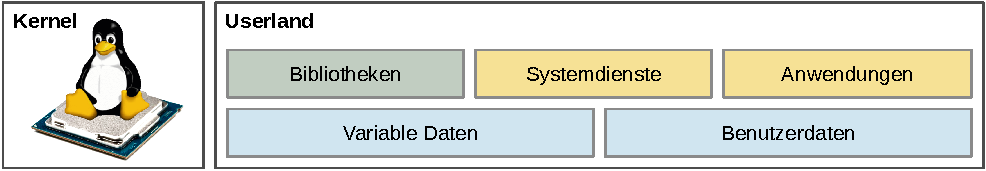
\includegraphics[width=\textwidth]{img/linux-bestandteile}
\end{frame}
}

%%% Folie
{
\scriptsize

\begin{frame}[allowframebreaks]{Der Linux Filesystem Hierarchy Standard}
    \begin{center}
        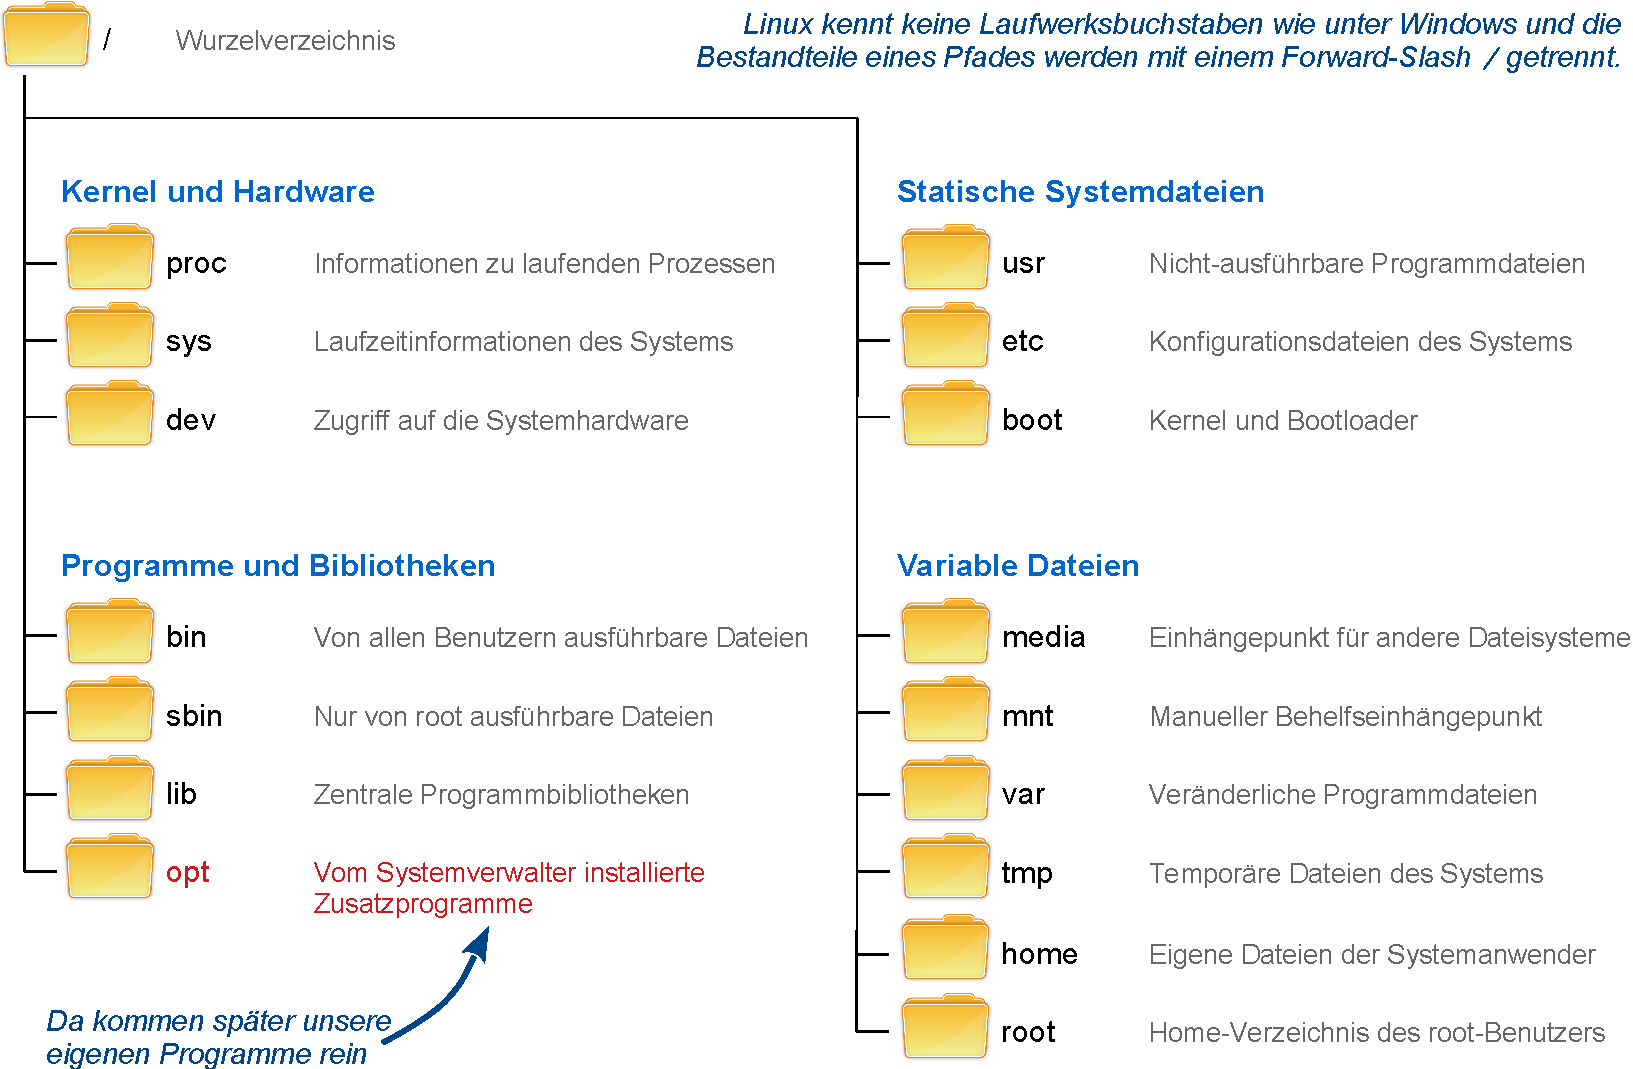
\includegraphics[width=\textwidth]{img/fhs-verzeichnisse}
    \end{center}

    \framebreak

    \begin{columns}[T]
        \column{.8\textwidth}
        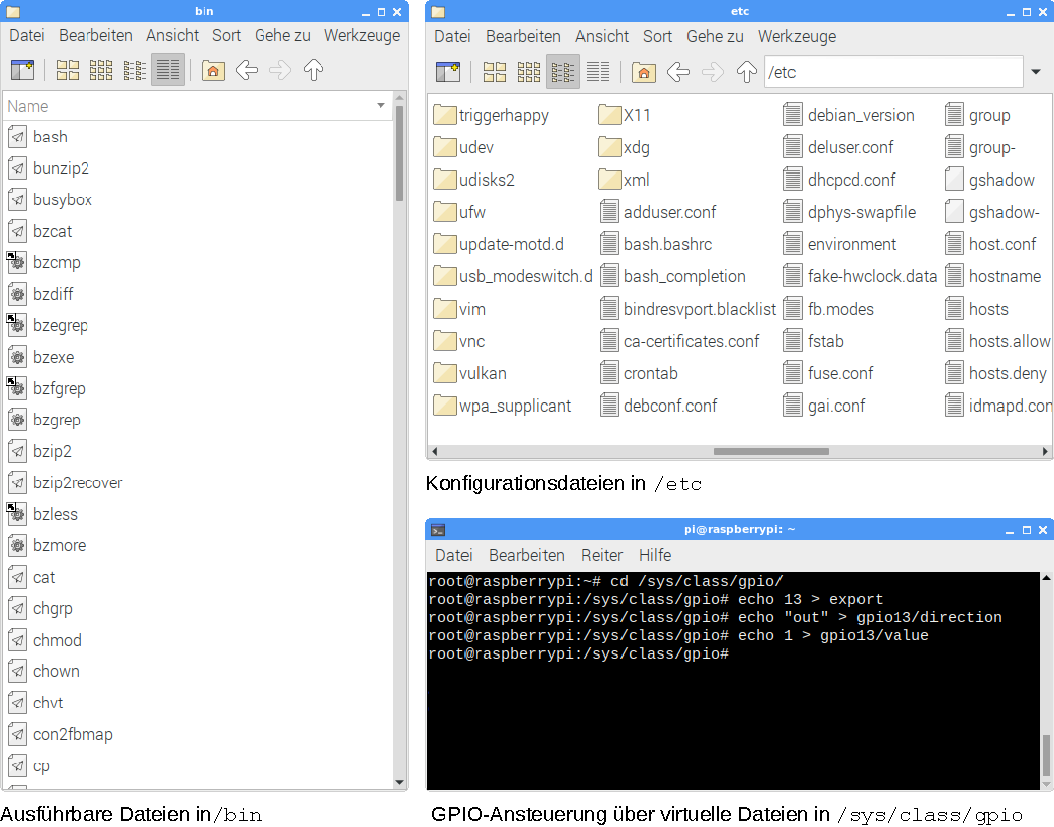
\includegraphics[width=\textwidth]{img/fhs-beispiele}

        \column{.3\textwidth}
        \Justified{
            Aufgrund der konzeptionellen Nähe zu Unix ist unter Linux fast alles
            eine Datei.
            \smallskip

            Die Konfiguration des Systems erfolgt deshalb genau so
            durch Editieren von Konfigurationsdateien, wie der Zugriff auf einen
            Hardwarebaustein nicht viel mehr als das Lesen und Schreiben virtueller
            Dateien erfordert.
        }
    \end{columns}
\end{frame}
}

%%% Folie
{
\scriptsize

\begin{frame}[allowframebreaks]{Fallbeispiel: Systembenutzer unter Linux}
    \begin{center}
        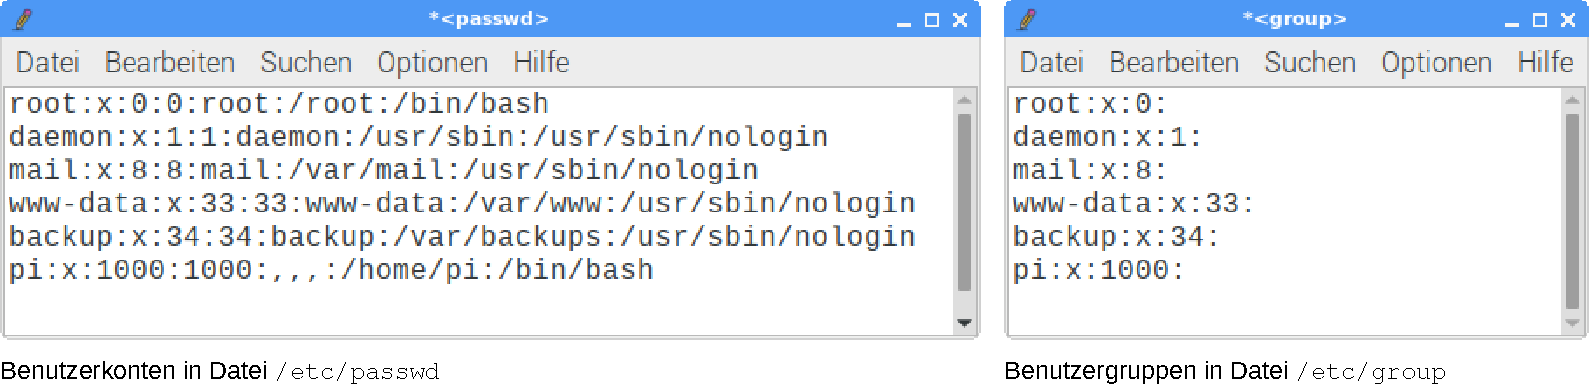
\includegraphics[width=\textwidth]{img/rechte-konfiguration}
    \end{center}

    \Justified{
        Die Benutzerkonten und Benutzergruppen sind in den Dateien
        \texttt{/etc/passwd} und \texttt{/etc/group} definiert. Jeder
        Benutzer bzw. jede Benutzergruppe bekommt hier eine numerische ID
        zugewiesen, die sehr oft nach folgendem Schema vergeben wird:
    }

    \medskip

    {
        \scriptsize
        \renewcommand{\arraystretch}{1.4}
        \setlength{\tabcolsep}{0em}

        \begin{tabularx}{\textwidth}{p{.11\textwidth} p{.2\textwidth} X}
            \hline
            \textbf{UID/GID} & \textbf{Bezeichnung} & \textbf{Bedeutung} \\
            \hline

            0 & Benutzer \texttt{root} & Superuser mit maximalen Berechtigungen \\
            1 -- 999 & Systembenutzer & Technische Benutzer zur Ausführung der Systemdienste \\
            $\geq$ 1000 & Interaktive Benutzer & Menschliche Benutzer mit Login-Möglichkeit \\
            \hline
        \end{tabularx}
    }

    \medskip
    \textbf{Wichtige Befehle}
    {
        \setlength{\leftmargini}{1.2em}
        \begin{columns}[T, onlytextwidth]
            \column{.5\textwidth}
            \begin{itemize}
                \item \texttt{adduser}: Neues Benutzerkonto anlegen
                \item \texttt{deluser}: Benutzerkonto löschen
                \item \texttt{usermod}: Benutzerkonte bearbeiten
            \end{itemize}

            \column{.5\textwidth}
            \begin{itemize}
                \item \texttt{passwd}: Benutzerpasswort ändern
                \item \texttt{groupadd}: Neue Benutzergruppe anlegen
                \item \texttt{delgroup}: Benutzergruppe löschen
            \end{itemize}
        \end{columns}
    }

    %%%
    \framebreak

    \begin{columns}[onlytextwidth]
        \column{.55\textwidth}
        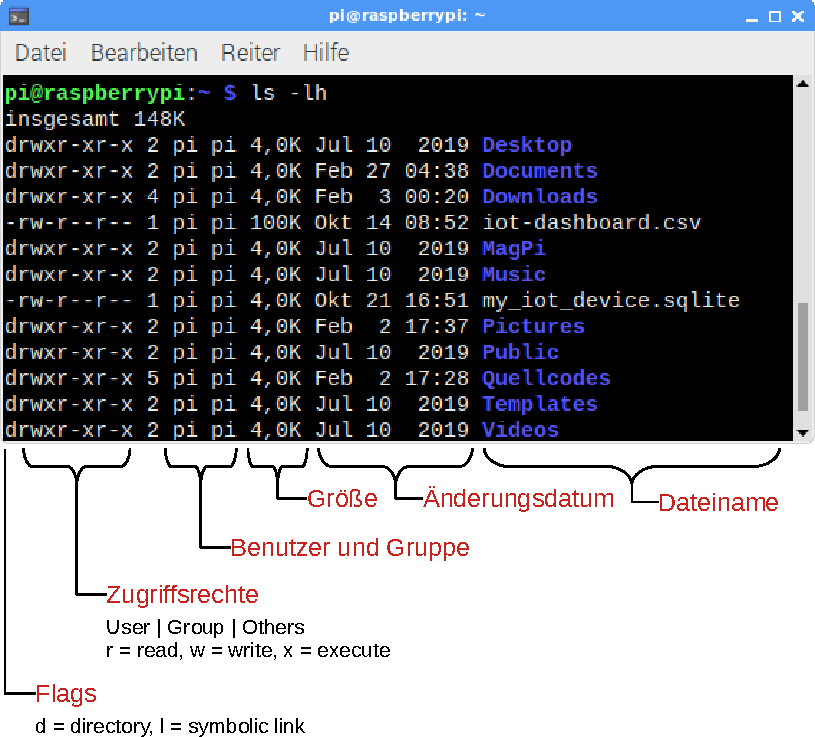
\includegraphics[width=\textwidth]{img/rechte-dateizugriff}

        \column{.4\textwidth}
        \Justified{
            Alle Einträge im Dateisystem sind immer genau einem Benutzerkonto
            und einer Benutzergruppe zugeordnet. Zusätzlich besitzen sie ein
            Bit-Feld mit Zugriffsrechten für

            \begin{itemize}
                \item den Benutzer,
                \item die Benutzergruppe,
                \item den Rest der Welt.
            \end{itemize}

            Über dieses Feld wird gesteuert, ob \mbox{Lese-,} Schreib- oder ausführende
            Zugriffe erlaubt sind.

            \medskip

            \glqq{}Ausführen\grqq{} bedeutet bei einer Datei, diese als Programm
            zu starten. Bei einem Verzeichnis bedeutet es, die Inhalte des
            Verzeichnisses zu sehen.

            \medskip

            Die Berechtigungsprüfung wird immer mit dem Benutzerkonto durchgeführt,
            unter dessen Namen ein zugreifendes Programm läuft.
        }
    \end{columns}

    \bigskip
    \textbf{Wichtige Befehle}
    \medskip

    \begin{columns}[onlytextwidth]
        \column{.3\textwidth}
        \texttt{chown} \\ Benutzer/Gruppe ändern

        \column{.3\textwidth}
        \texttt{chmod} \\ Zugriffsrechte ändern

        \column{.4\textwidth}
        \texttt{sudo} \\ Programm mit anderem Benutzer starten
    \end{columns}
\end{frame}
}

%%% Folie
{
\scriptsize

\begin{frame}{Fallbeispiel: Automatischer Start eines Pythonprogramms}
    \begin{columns}[onlytextwidth]
        \column{.58\textwidth}
        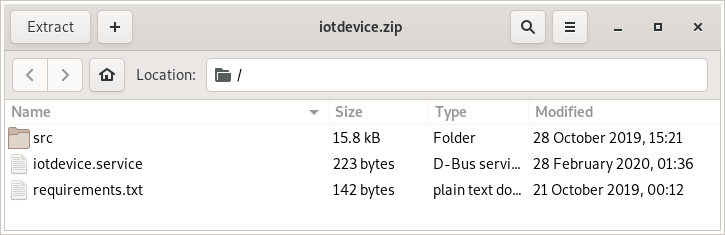
\includegraphics[width=\textwidth]{img/systemd-beispiel-zipfile}

        \column{.4\textwidth}
        \Justified{
            Eine Python-Anwendung soll im Rasbperry Pi OS systemweit installiert
            und beim Hochfahren automatisch gestartet werden. Die Desktop-Umgebung
            (sofern installiert) soll aus Performancegründen deaktiviert werden.
        }
    \end{columns}

    \bigskip
    \textbf{Inhalt der Datei \texttt{iotdevice.service}}
    \lstinputlisting[language=Config]{code/iotdevice.service}

    \medskip
    \textbf{Auszuführende Befehle}
    \vskip -.5em
    \begin{columns}[onlytextwidth]
        \column{.5\textwidth}
        \lstinputlisting[language=Config, linerange={1-8}]{code/iotdevice.install.sh}

        \column{.5\textwidth}
        \lstinputlisting[language=Config, linerange={9-16}, firstnumber=9]{code/iotdevice.install.sh}
    \end{columns}
\end{frame}
}

%-------------------------------------------------------------------------------
\section{Remote-Entwicklung mit VS Code}
%-------------------------------------------------------------------------------

%%% Folien
{
\scriptsize
\setlength{\fboxsep}{0pt}

\begin{frame}[allowframebreaks]{Testen der SSH-Verbindung}
    \begin{center}
        \fbox{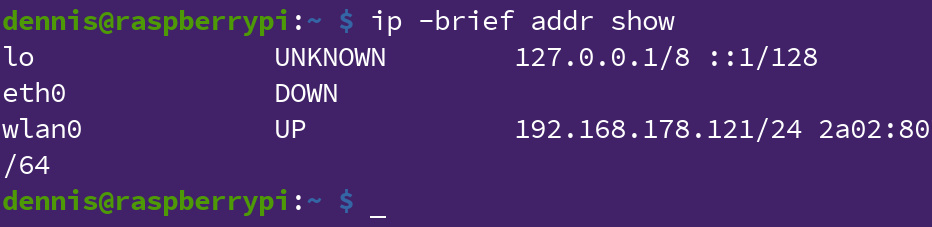
\includegraphics[width=\textwidth]{img/ssh-ip-addr-show}}
    \end{center}

    \Justified{
        Mit dem Befehl \texttt{ip -brief addr show} lassen sich die IP-Adressen des Raspberry Pi anzeigen.
        Diese werden für den Remote-Login mit SSH benötigt, um den Raspberry Pi auch ohne Bildschirm,
        Tastatur und Maus programmieren vom Laptop aus programmieren zu können.
    }

    %%%
    \framebreak

    \begin{center}
        \fbox{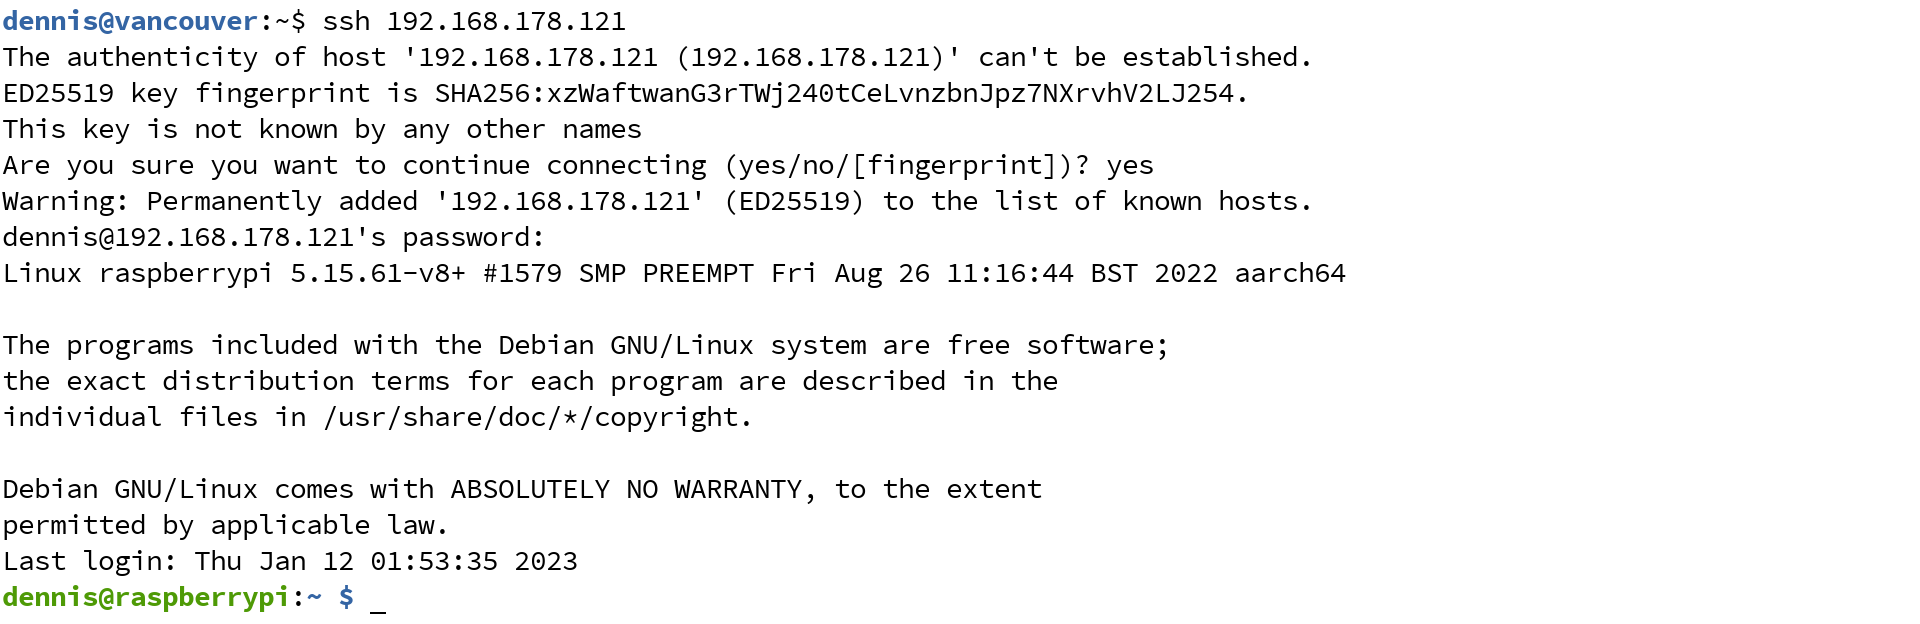
\includegraphics[width=\textwidth]{img/ssh-erstlogon}}
    \end{center}

    \Justified{
        Auf dem eigenen Laptop kann der Logon mit folgendem Befehl getestet werden:
        \smallskip

        \texttt{ssh \textit{benutzername}@\textit{ip-adresse}}
        \smallskip

        Es sollten eine einmalige Sicherheitsabfrage sowie der Login-Prompt des Raspberry Pi
        erscheinen. An diesem sollte man sich mit dem während der Installation angelegten
        Benutzerkonto anmelden können. Mit dem Befehl \texttt{exit} kann die Anmeldung
        danach beendet werden.
        \smallskip

        \textcolor{MidnightBlue}{
            Da sich die IP-Adresse jederzeit ändern kann, werden wir demnächst das Werkzeug
            \textbf{find-my-device} auf dem Raspberry Pi installieren. Damit lässt sich die
            IP-Adresse dann ganz einfach durch Aufrufen einer Webseite ermitteln. Das Werkzeug
            programmiere ich gerade. \smiley{}
            \smallskip
        }

        \textcolor{darkred}{
            Zum Ausschalten führen Sie den Befehl \texttt{sudo poweroff} aus, bevor Sie den
            Strom trennen. EIn hartes Ausschalten ohne diesen Befehl ist nur erlaubt, wenn
            das Dateisystem read-only eingehängt wurde, um Datenverluste zu vermeiden!
        }
    }
\end{frame}
}

%%%%%%%
% TODO: Folien zu "Find my Device"
%%%%%%%

%%% Folien
{
\scriptsize
\setlength{\fboxsep}{0pt}

\begin{frame}[allowframebreaks, fragile]{Remote-Verbindung herstellen}
    \begin{columns}
        \column[c]{.6\textwidth}
        \fbox{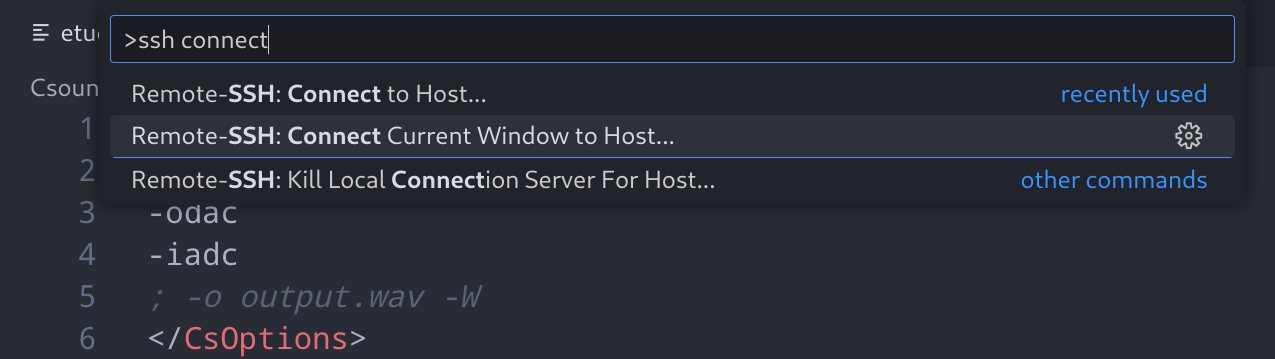
\includegraphics[width=\textwidth]{img/vscode-01}}

        \fbox{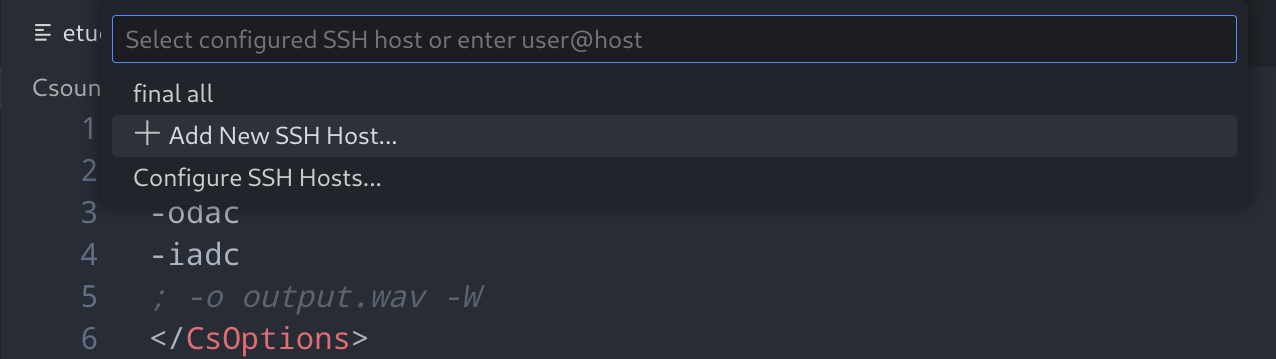
\includegraphics[width=\textwidth]{img/vscode-02}}

        \fbox{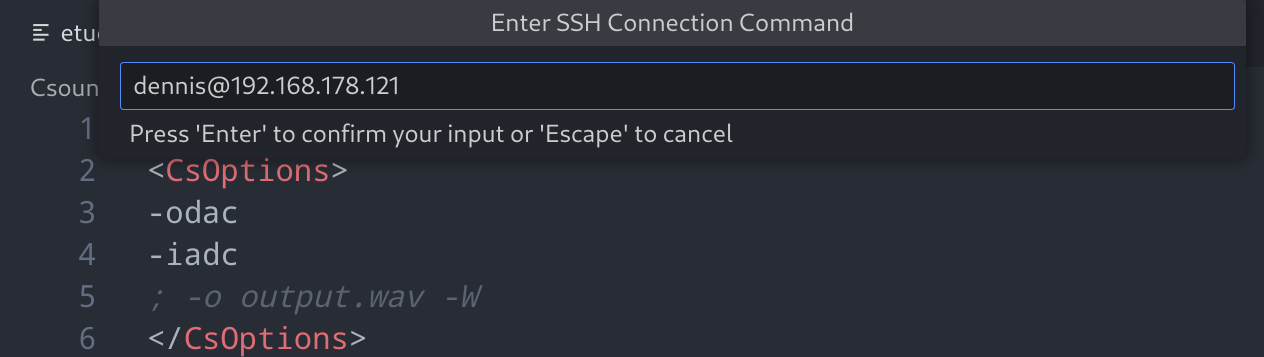
\includegraphics[width=\textwidth]{img/vscode-03}}

        \column[c]{.4\textwidth}
        \Justified{
            Zunächst muss eine neue SSH-Verbindung angelegt werden:
        }

        \begin{enumerate}
            \item Kommandopalette öffnen mit \texttt{Shift+Strg+P}
            \item Nach ,,Remote-SSH'' suchen
            \item Den Eintrag ,,Connect Current Window To Host...'' auswählen
            \item Für die Verbundungsdaten \texttt{\textit{benutzername}@\textit{ip-adresse}} eingeben
        \end{enumerate}
    \end{columns}

    %%%
    \framebreak

    \begin{columns}
        \column[c]{.6\textwidth}
        \fbox{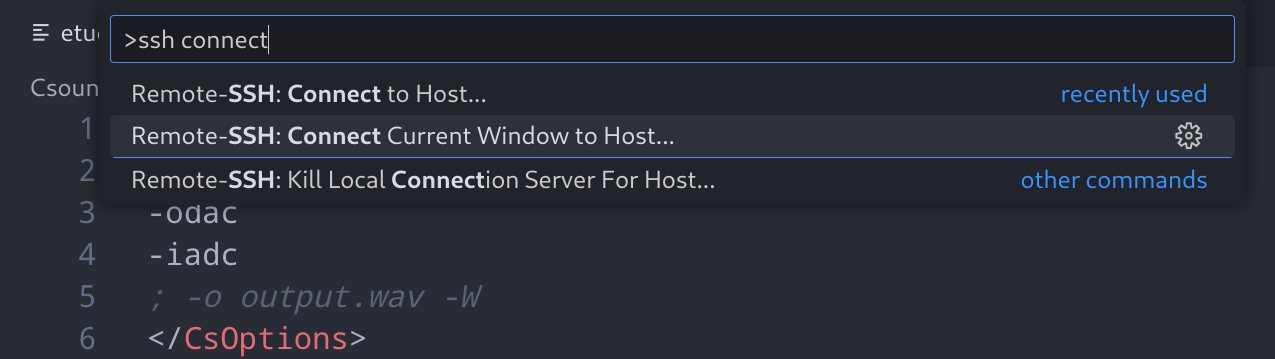
\includegraphics[width=\textwidth]{img/vscode-01}}

        \fbox{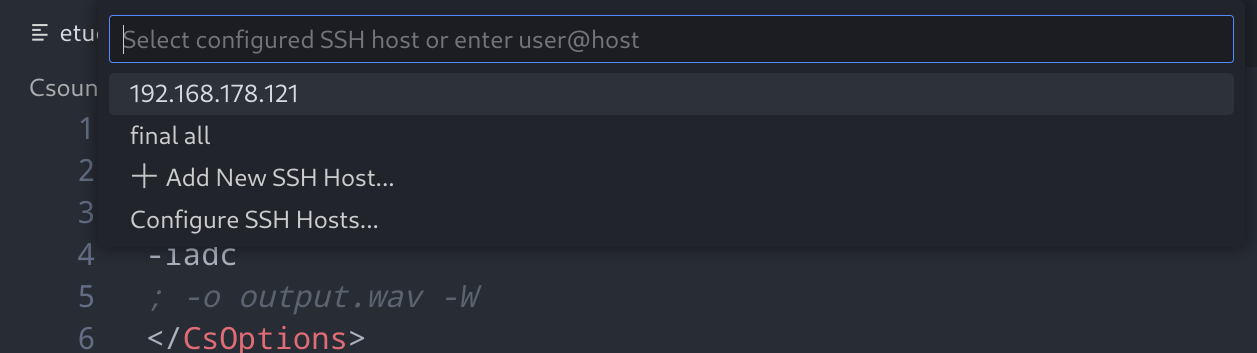
\includegraphics[width=\textwidth]{img/vscode-04}}

        \fbox{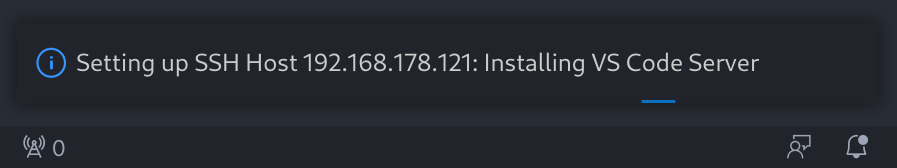
\includegraphics[width=\textwidth]{img/vscode-05}}

        \fbox{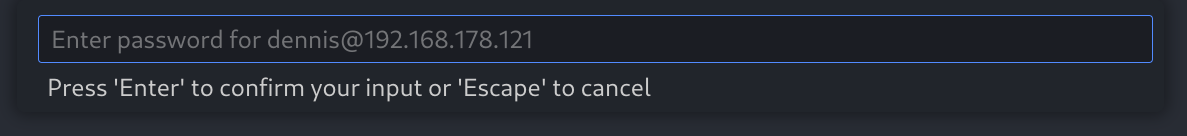
\includegraphics[width=\textwidth]{img/vscode-06}}

        \column[c]{.4\textwidth}
        \Justified{
            Anschließend kann die eben angelegte Verbindung hergestellt werden:
        }

        \begin{enumerate}
            \item Kommandopalette öffnen mit \texttt{Shift+Strg+P}
            \item Erneut nach ,,Remote-SSH'' suchen und ,,Connect Current Window To Host...'' auswählen
            \item Die eben angelegte Verbindung anklicken
            \item Auf Nachfrage das Benutzerpasswort eingeben
            \item Abwarten, bis der Workspace auf dem Raspberry Pi eingerichtet wurde
        \end{enumerate}
    \end{columns}
\end{frame}
}

%%% Folien
{
\scriptsize
\setlength{\fboxsep}{0pt}

\begin{frame}[allowframebreaks, fragile]{Fallbeispiel: Hallo, Raspberry Pi}
    \begin{center}
        \fbox{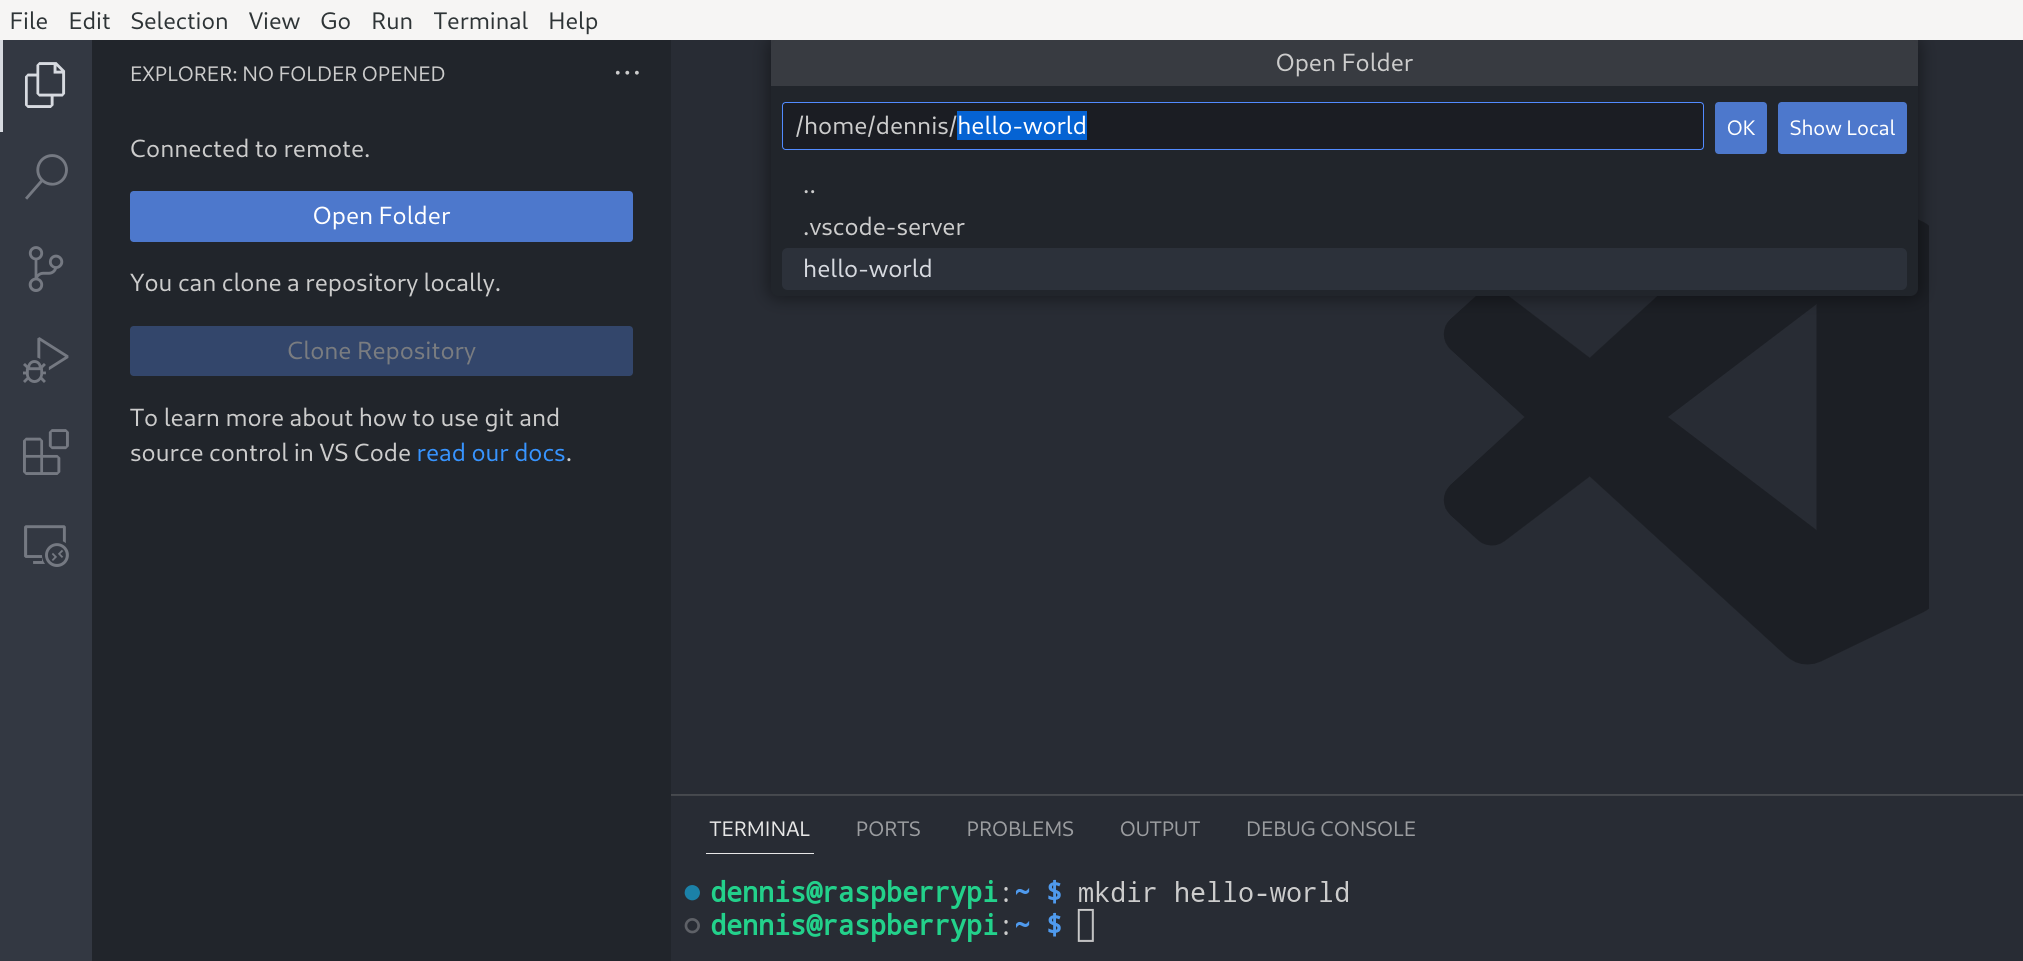
\includegraphics[width=.9\textwidth]{img/vscode-07}}
    \end{center}

    \Justified{
        Mit \texttt{Strg+Ö} (wie englisch ,,Törminal'' \smiley{}) kann eine Konsole geöffnet werden,
        um Befehle auf dem Raspberry Pi auszuführen. Der Befehl \texttt{mkdir \textit{verzeichnis}}
        legt ein neues Quellcodeverzeichnis an, das anschließen über den Button ,,Open Folder''
        im linken Bereich geöffnet werden kann.
    }

    %%%
    \framebreak

    \begin{columns}
        \column[c]{.6\textwidth}
        %~ \fbox{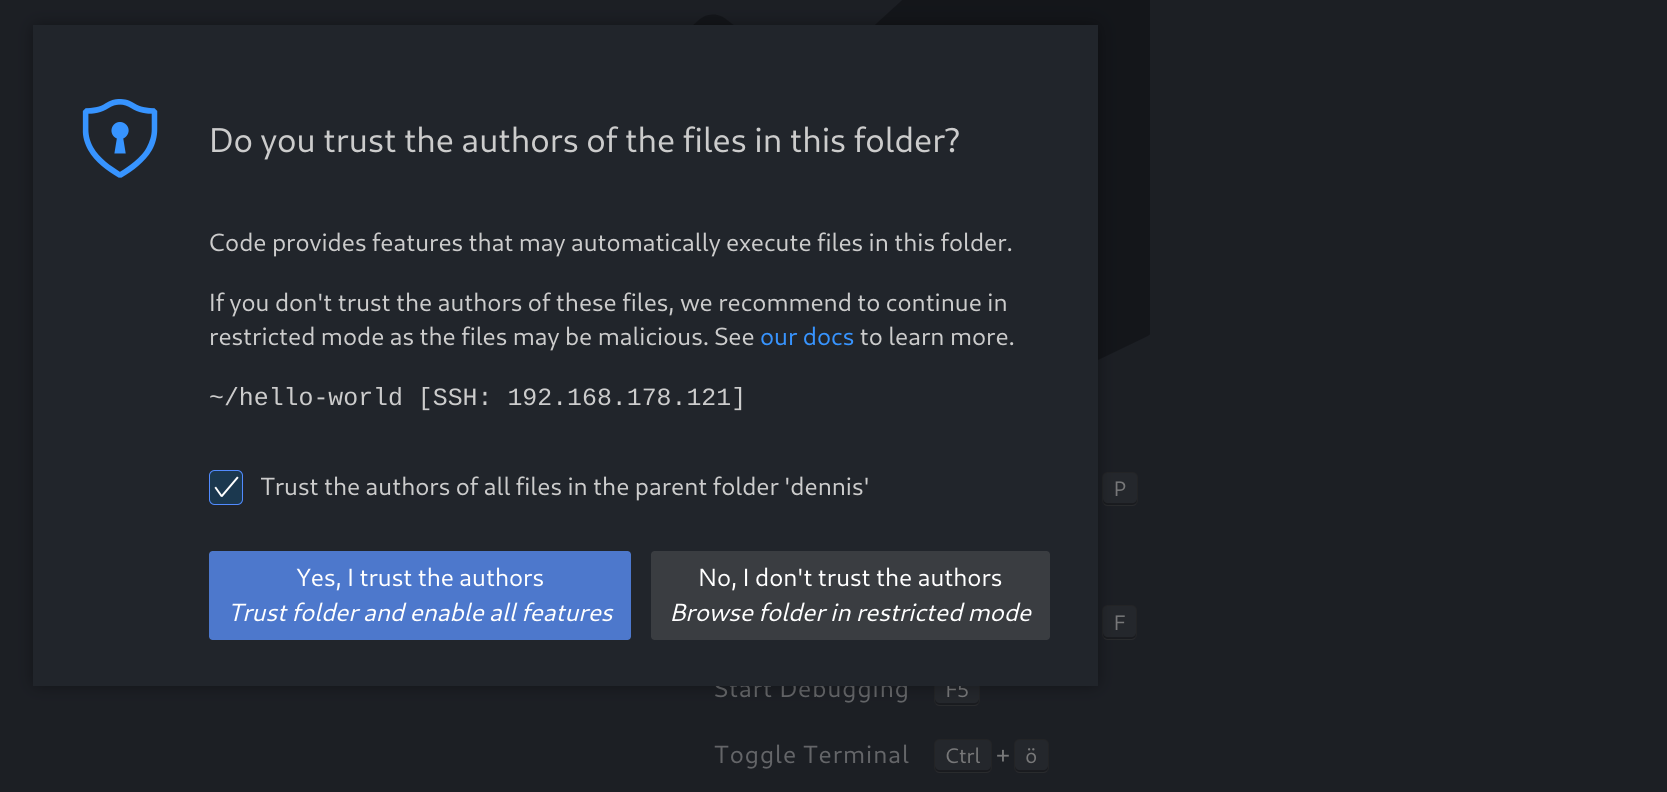
\includegraphics[width=\textwidth]{img/vscode-08}}

        \fbox{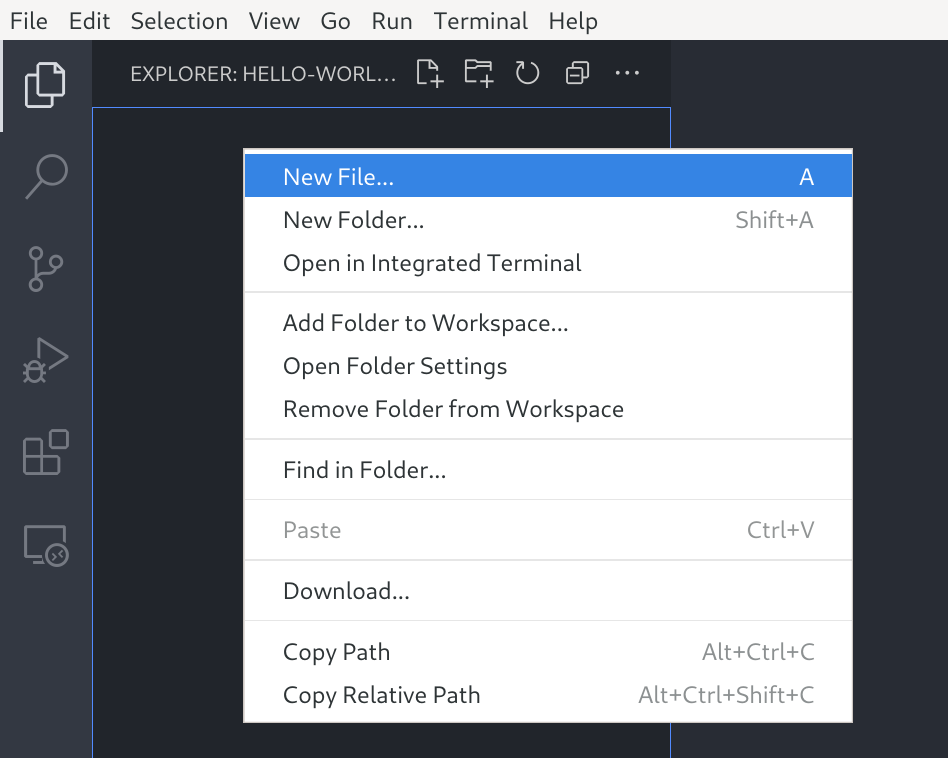
\includegraphics[width=\textwidth]{img/vscode-09}}

        \fbox{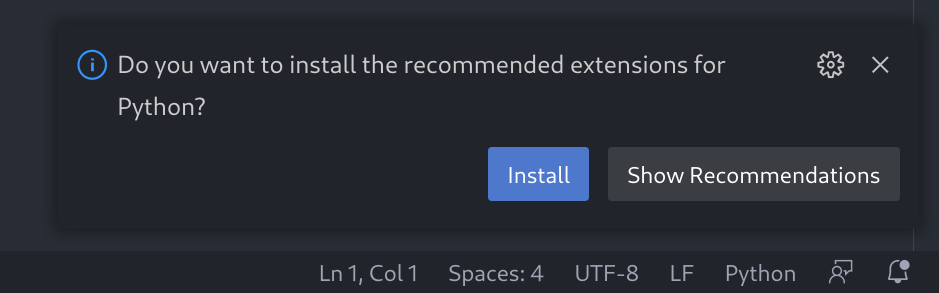
\includegraphics[width=\textwidth]{img/vscode-10}}

        \column[c]{.4\textwidth}
        \Justified{
            Weil das verzeichnis noch leer ist, werden links noch keine Dateien angezeigt.
            Mit Rechtsklick soll daher eine Datei namens \texttt{main.py} angelegt werden.
            \smallskip

            Die Frage, ob die empfohlenen Erweiterungen für die Pythonprogrammierung in
            Visual Studio Code installiert werden sollen, kann mit Klick auf ,,Install''
            bestätigt werden. Die Erweiterungen vereinfachen ein wenig das Programmieren
            durch Codeverschläge und Prüfungen.
        }
    \end{columns}

    %%%
    \framebreak

    \begin{columns}
        \column[c]{.54\textwidth}
        %~ \fbox{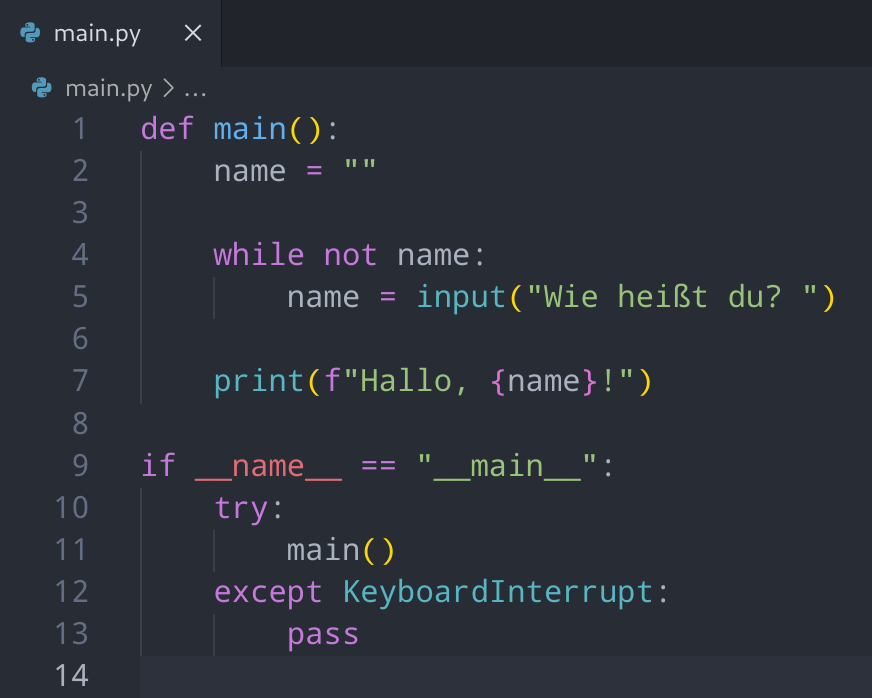
\includegraphics[width=\textwidth]{img/vscode-11}}

        \fbox{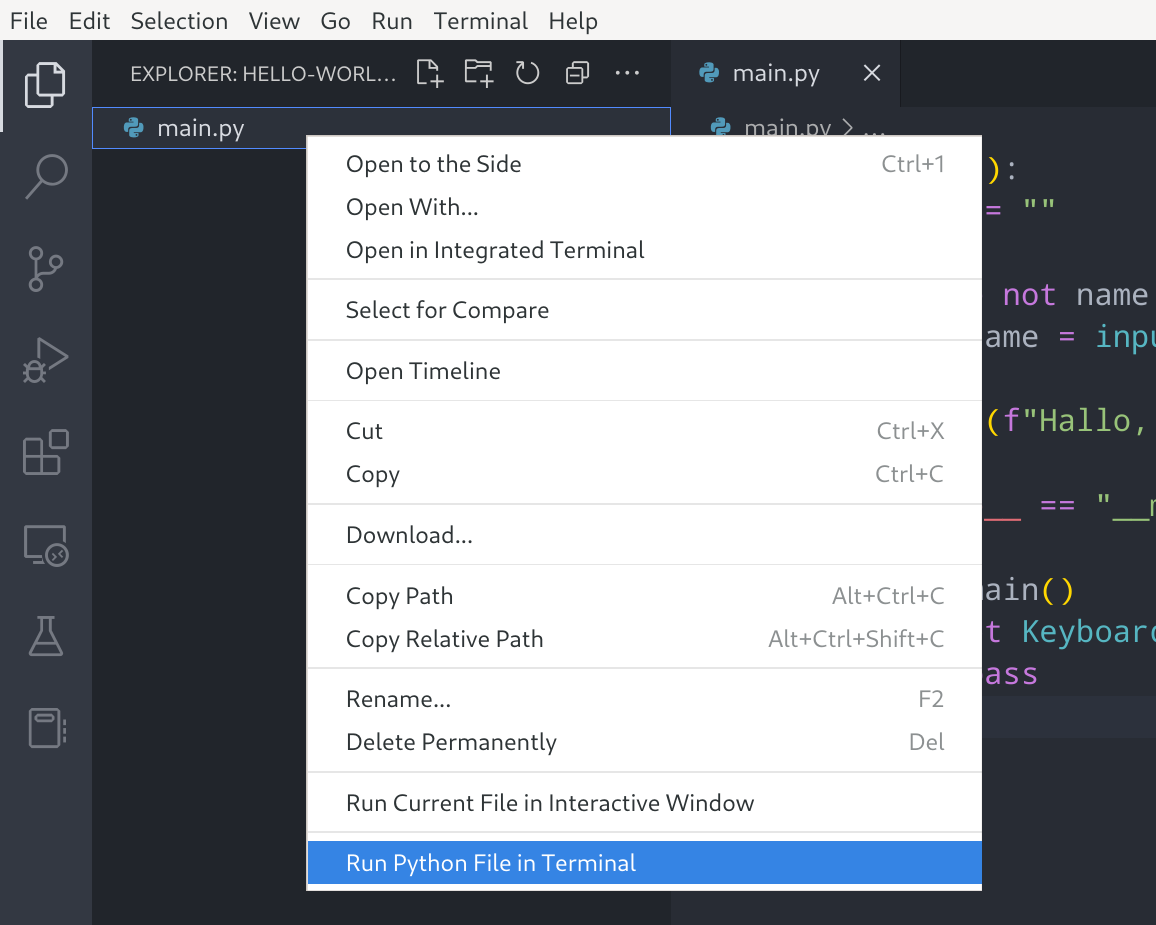
\includegraphics[width=\textwidth]{img/vscode-12}}

        \fbox{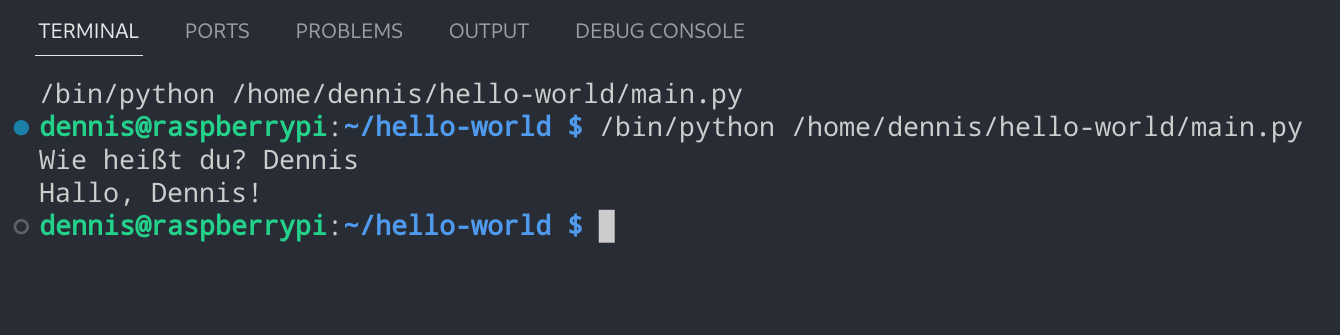
\includegraphics[width=\textwidth]{img/vscode-13}}

        \column[c]{.45\textwidth}
        \Justified{
            Die Datei soll folgenden Inhalt besitzen:
        }

        \begin{lstlisting}[language=Python, gobble=12]
            def main():
                name = ""

                while not name:
                    name = input("Wie heißt du? ")

                print(f"Hallo, {name}!")

            if __name__ == "__main__":
                try:
                    main()
                except KeyboardInterrupt:
                    pass
        \end{lstlisting}

        \bigskip

        \Justified{
            Über den Eintrag ,,Run Python File in Terminal'' im Kontextmenü (Rechtsklick)
            lässt sich das Programm ausführen. Das Ergebnis sollte wie im unteren Screenshot
            aussehen.
        }
    \end{columns}
\end{frame}
}

%-------------------------------------------------------------------------------
\section{Erste Schritte mit Python}
%-------------------------------------------------------------------------------

%%% Folie
\begin{frame}{ChatGPT über Python und Java}
    \begin{center}
        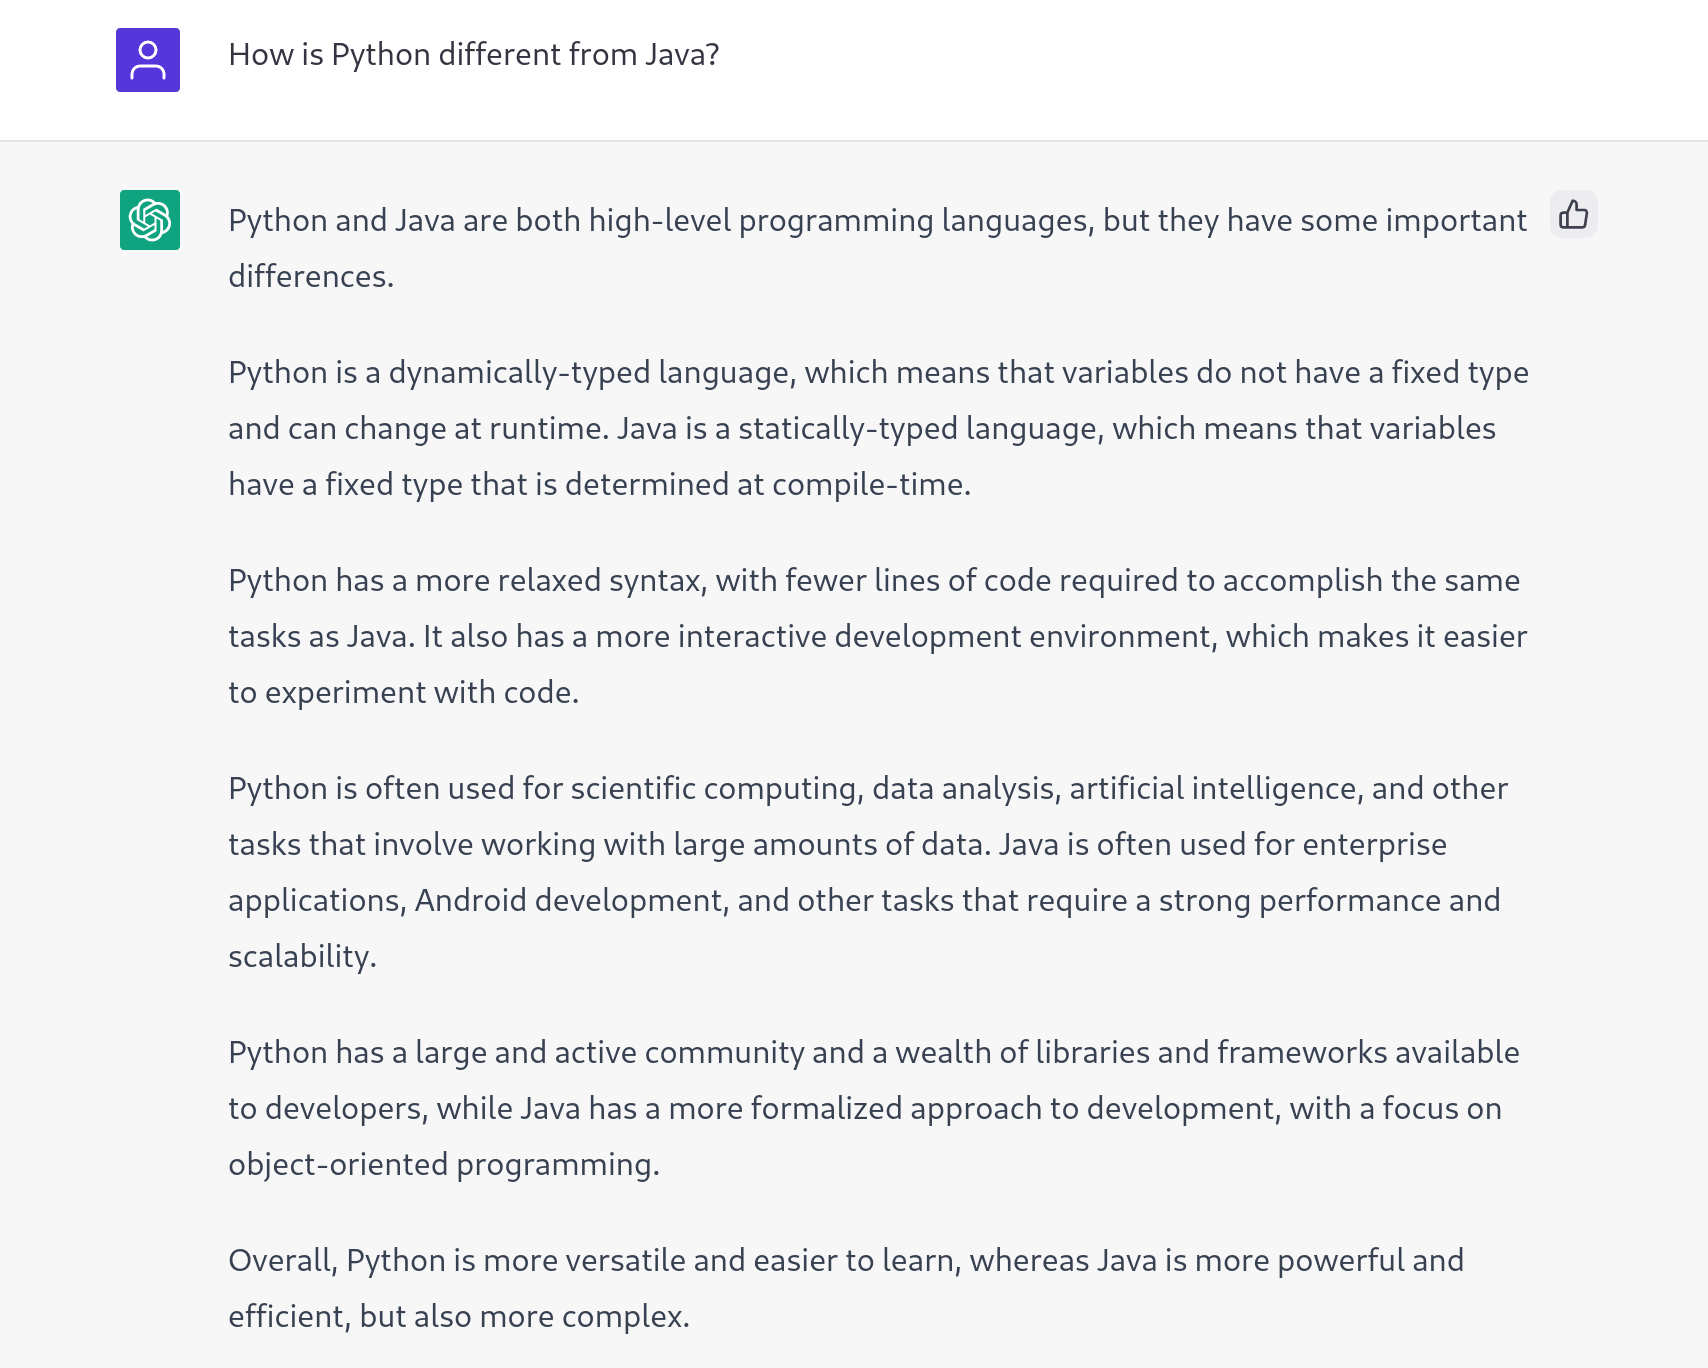
\includegraphics[width=.85\textwidth]{img/chatgpt-python-java}
    \end{center}
\end{frame}

%%% Folie
{
\footnotesize
\setlength{\fboxsep}{0pt}

\begin{frame}{Hilfreiche Webseiten über Python}
    \begin{columns}
        \column[T]{.33\textwidth}
        \fbox{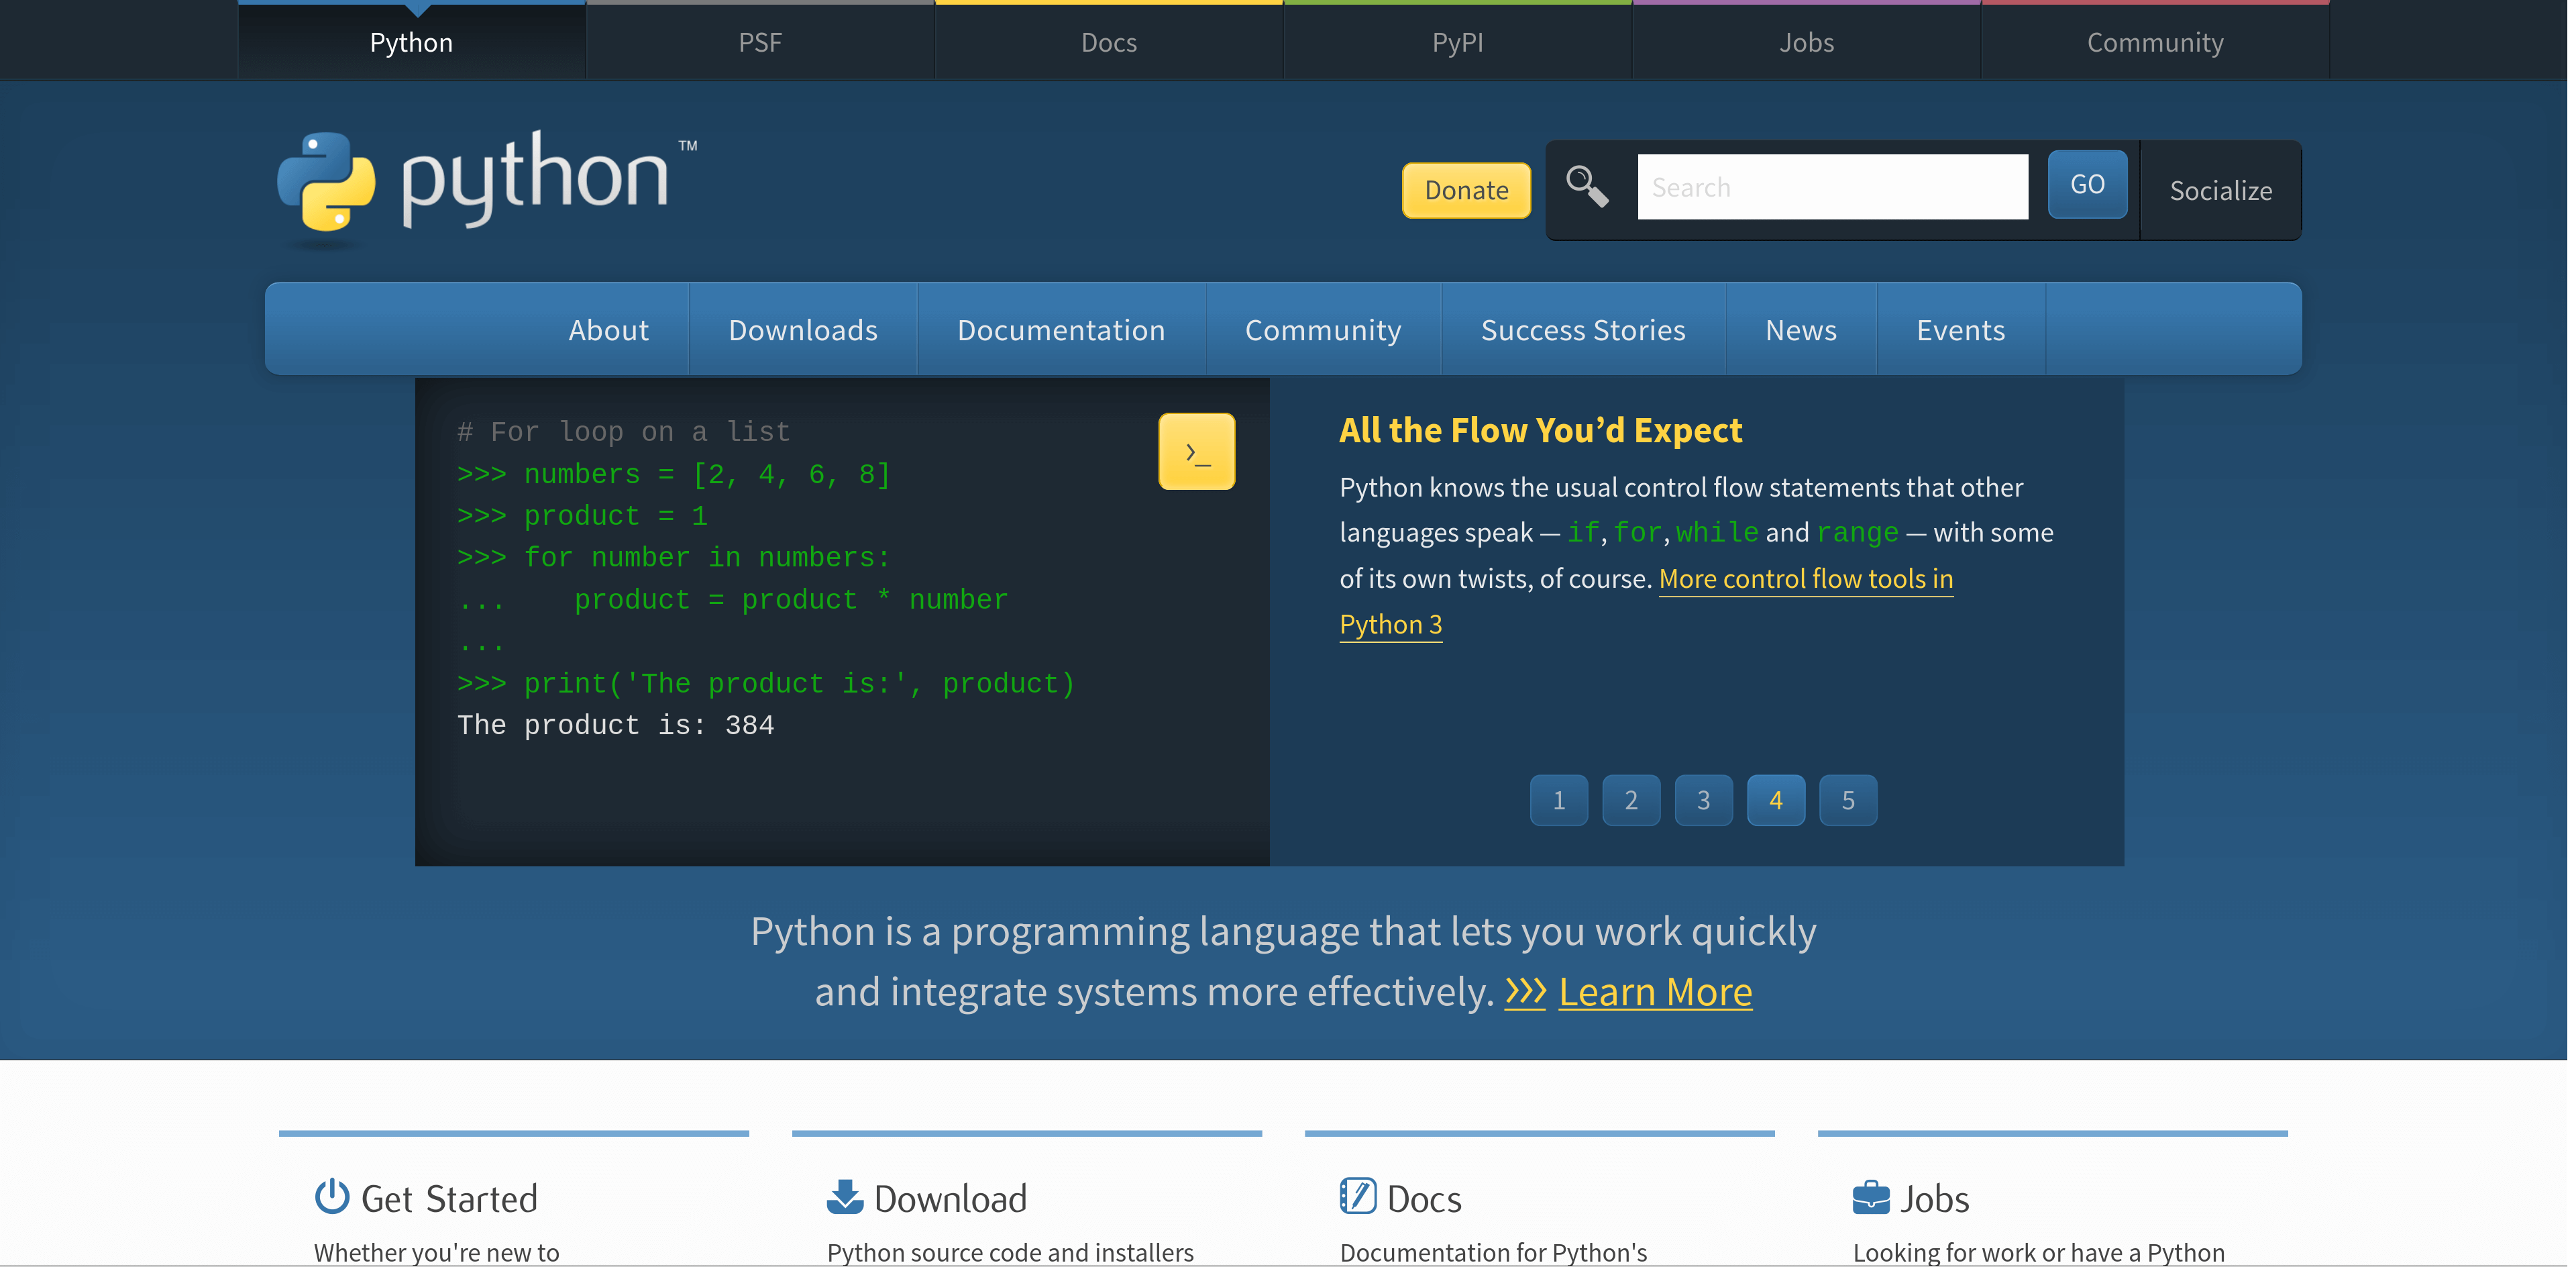
\includegraphics[width=\textwidth]{img/webseite-python}}
        \vskip .5em
        \textbf{Webseite von Python} \\
        \href{https://www.python.org/}{python.org}

        \column[T]{.33\textwidth}
        \fbox{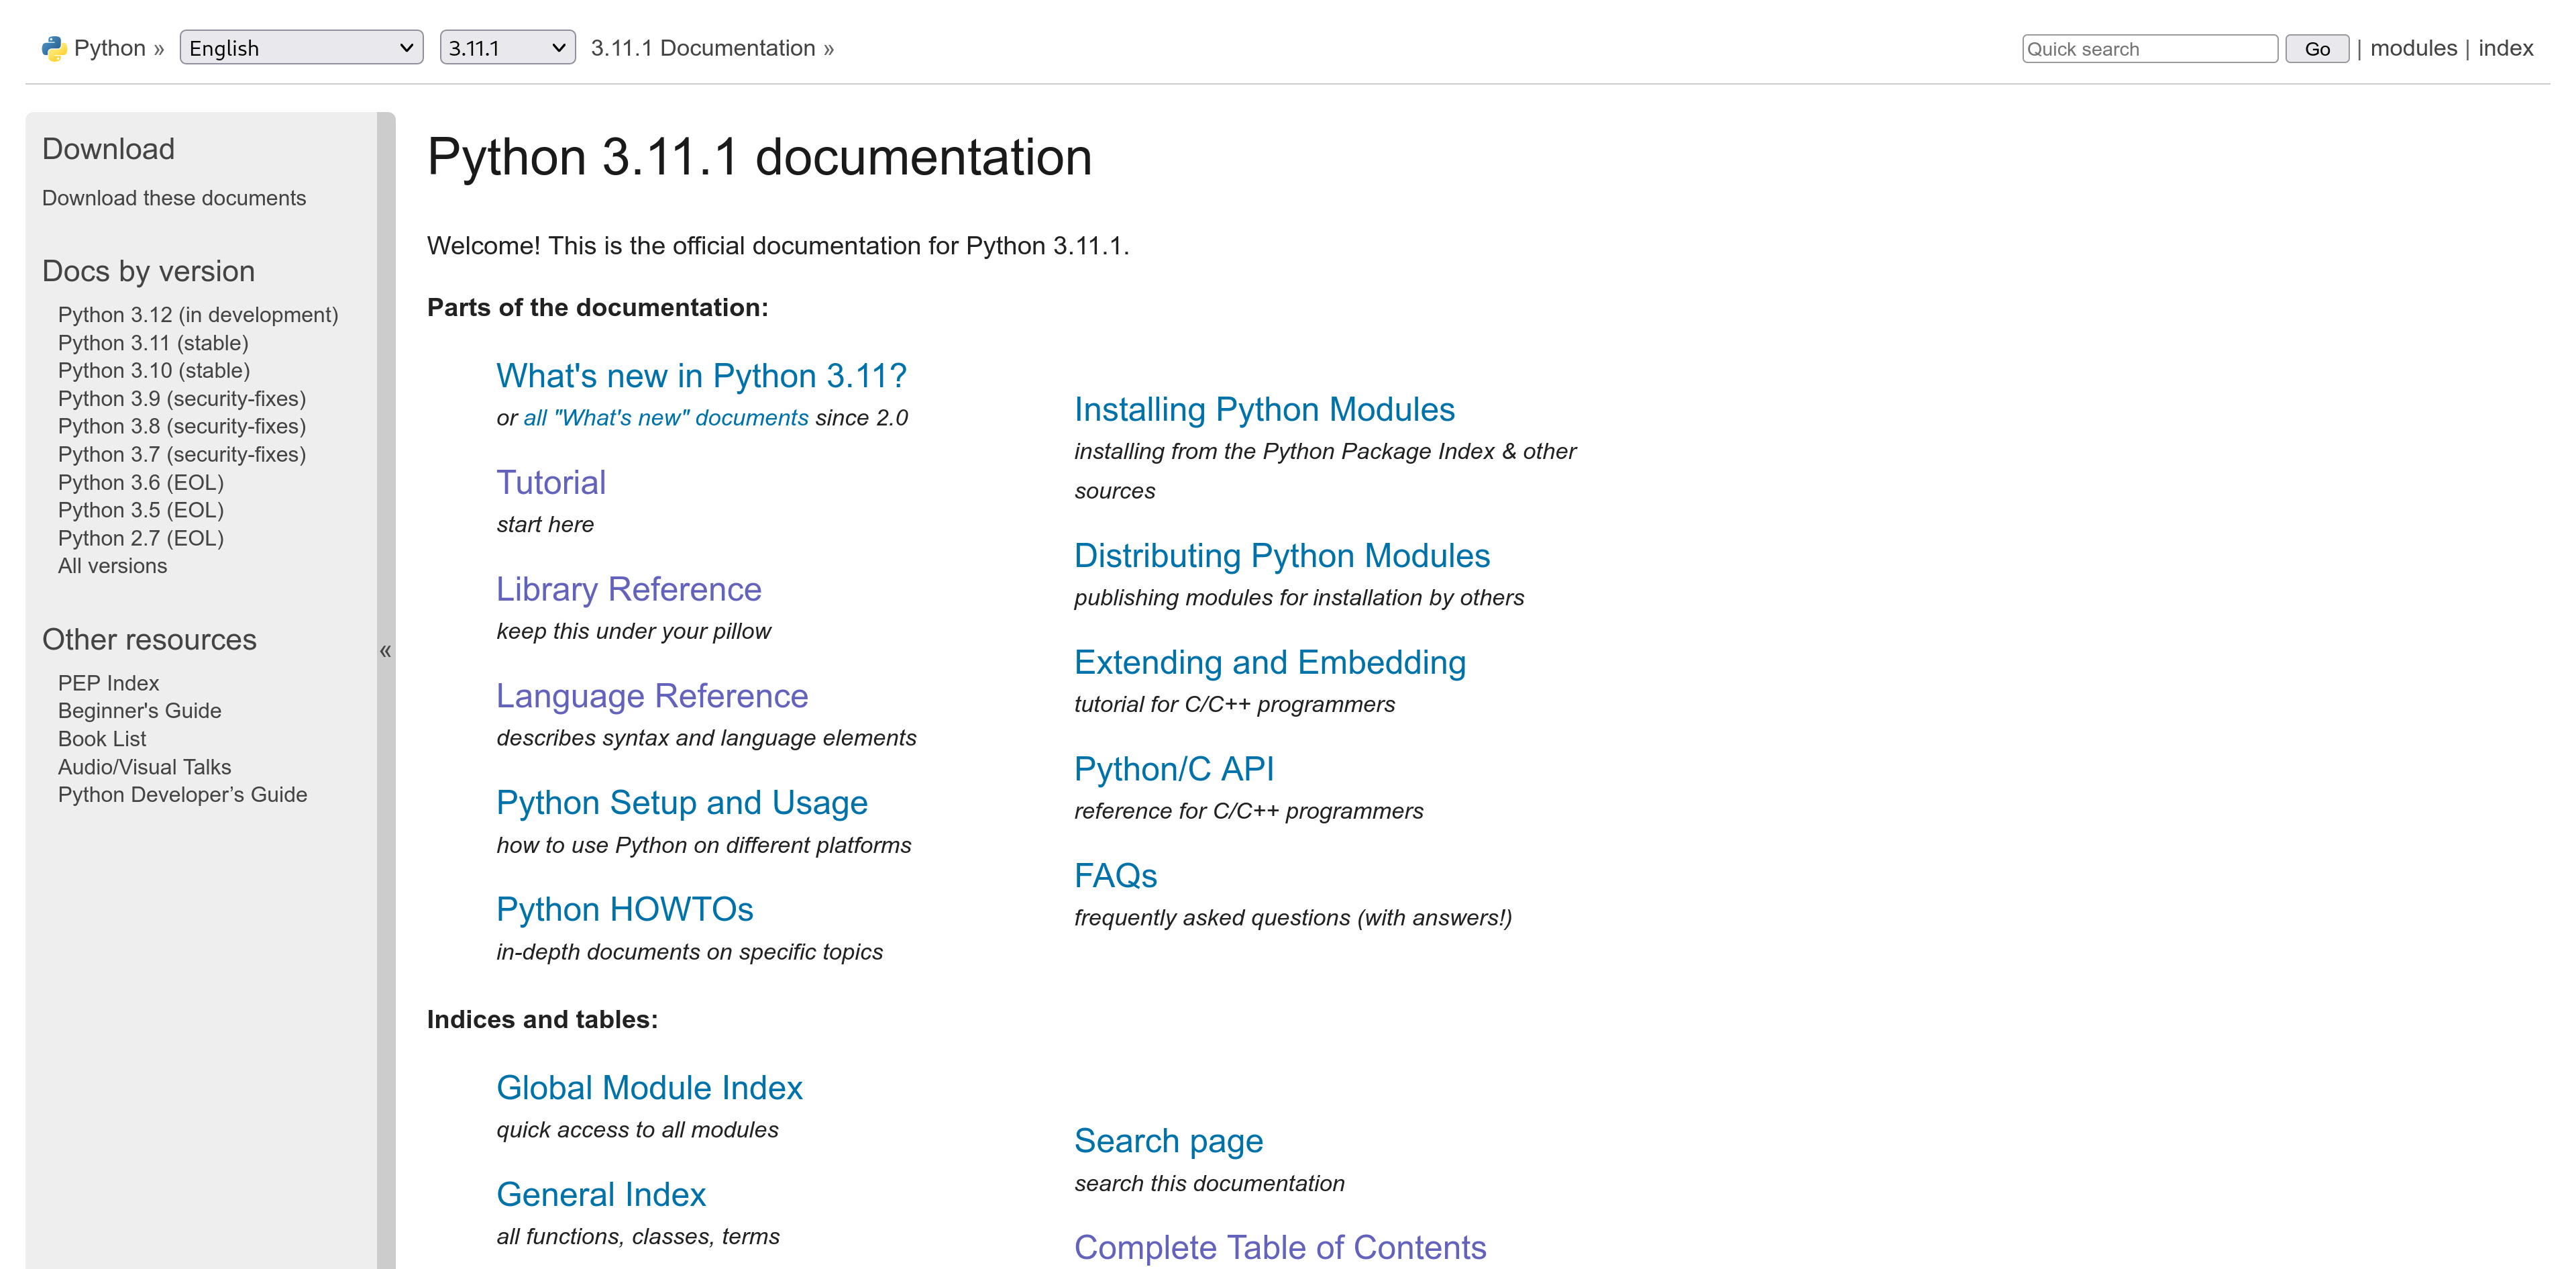
\includegraphics[width=\textwidth]{img/webseite-docs}}
        \vskip .5em
        \textbf{Offizielle Dokumentation} \\
        \href{https://docs.python.org/}{docs.python.org}

        \column[T]{.33\textwidth}
        \fbox{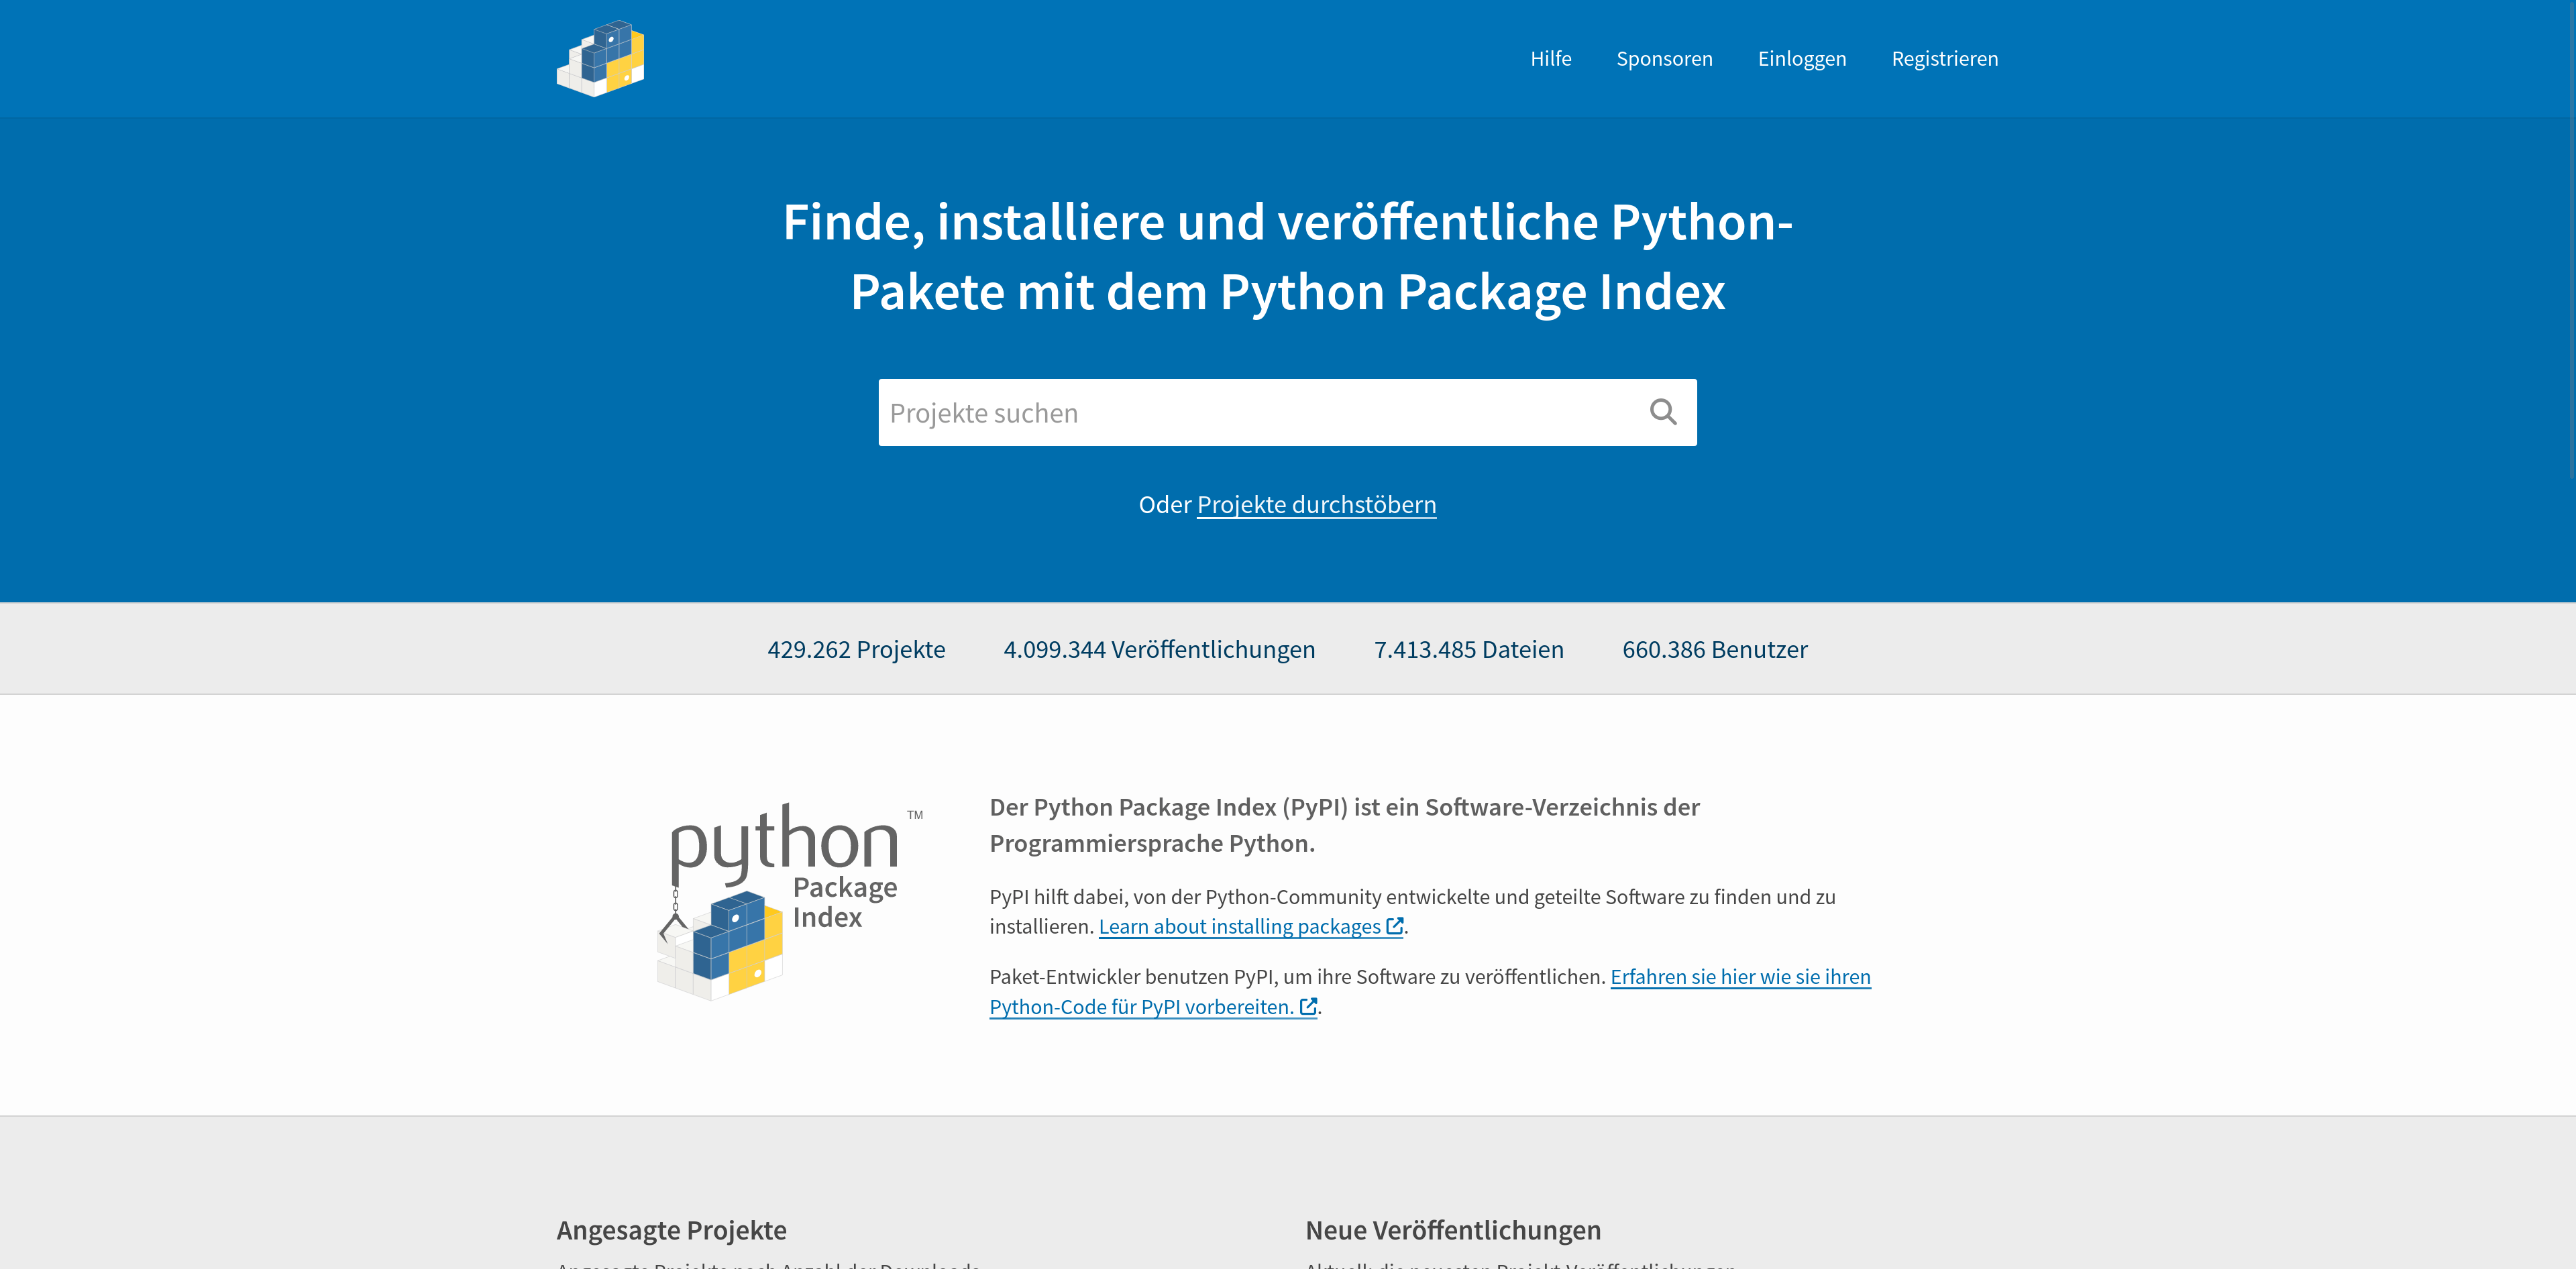
\includegraphics[width=\textwidth]{img/webseite-pypi}}
        \vskip .5em
        \textbf{Python Package Index} \\
        \href{https://pypi.org/}{pypi.org}
    \end{columns}

    \vskip 0.6cm

    \begin{columns}
        \column[T]{.33\textwidth}
        \fbox{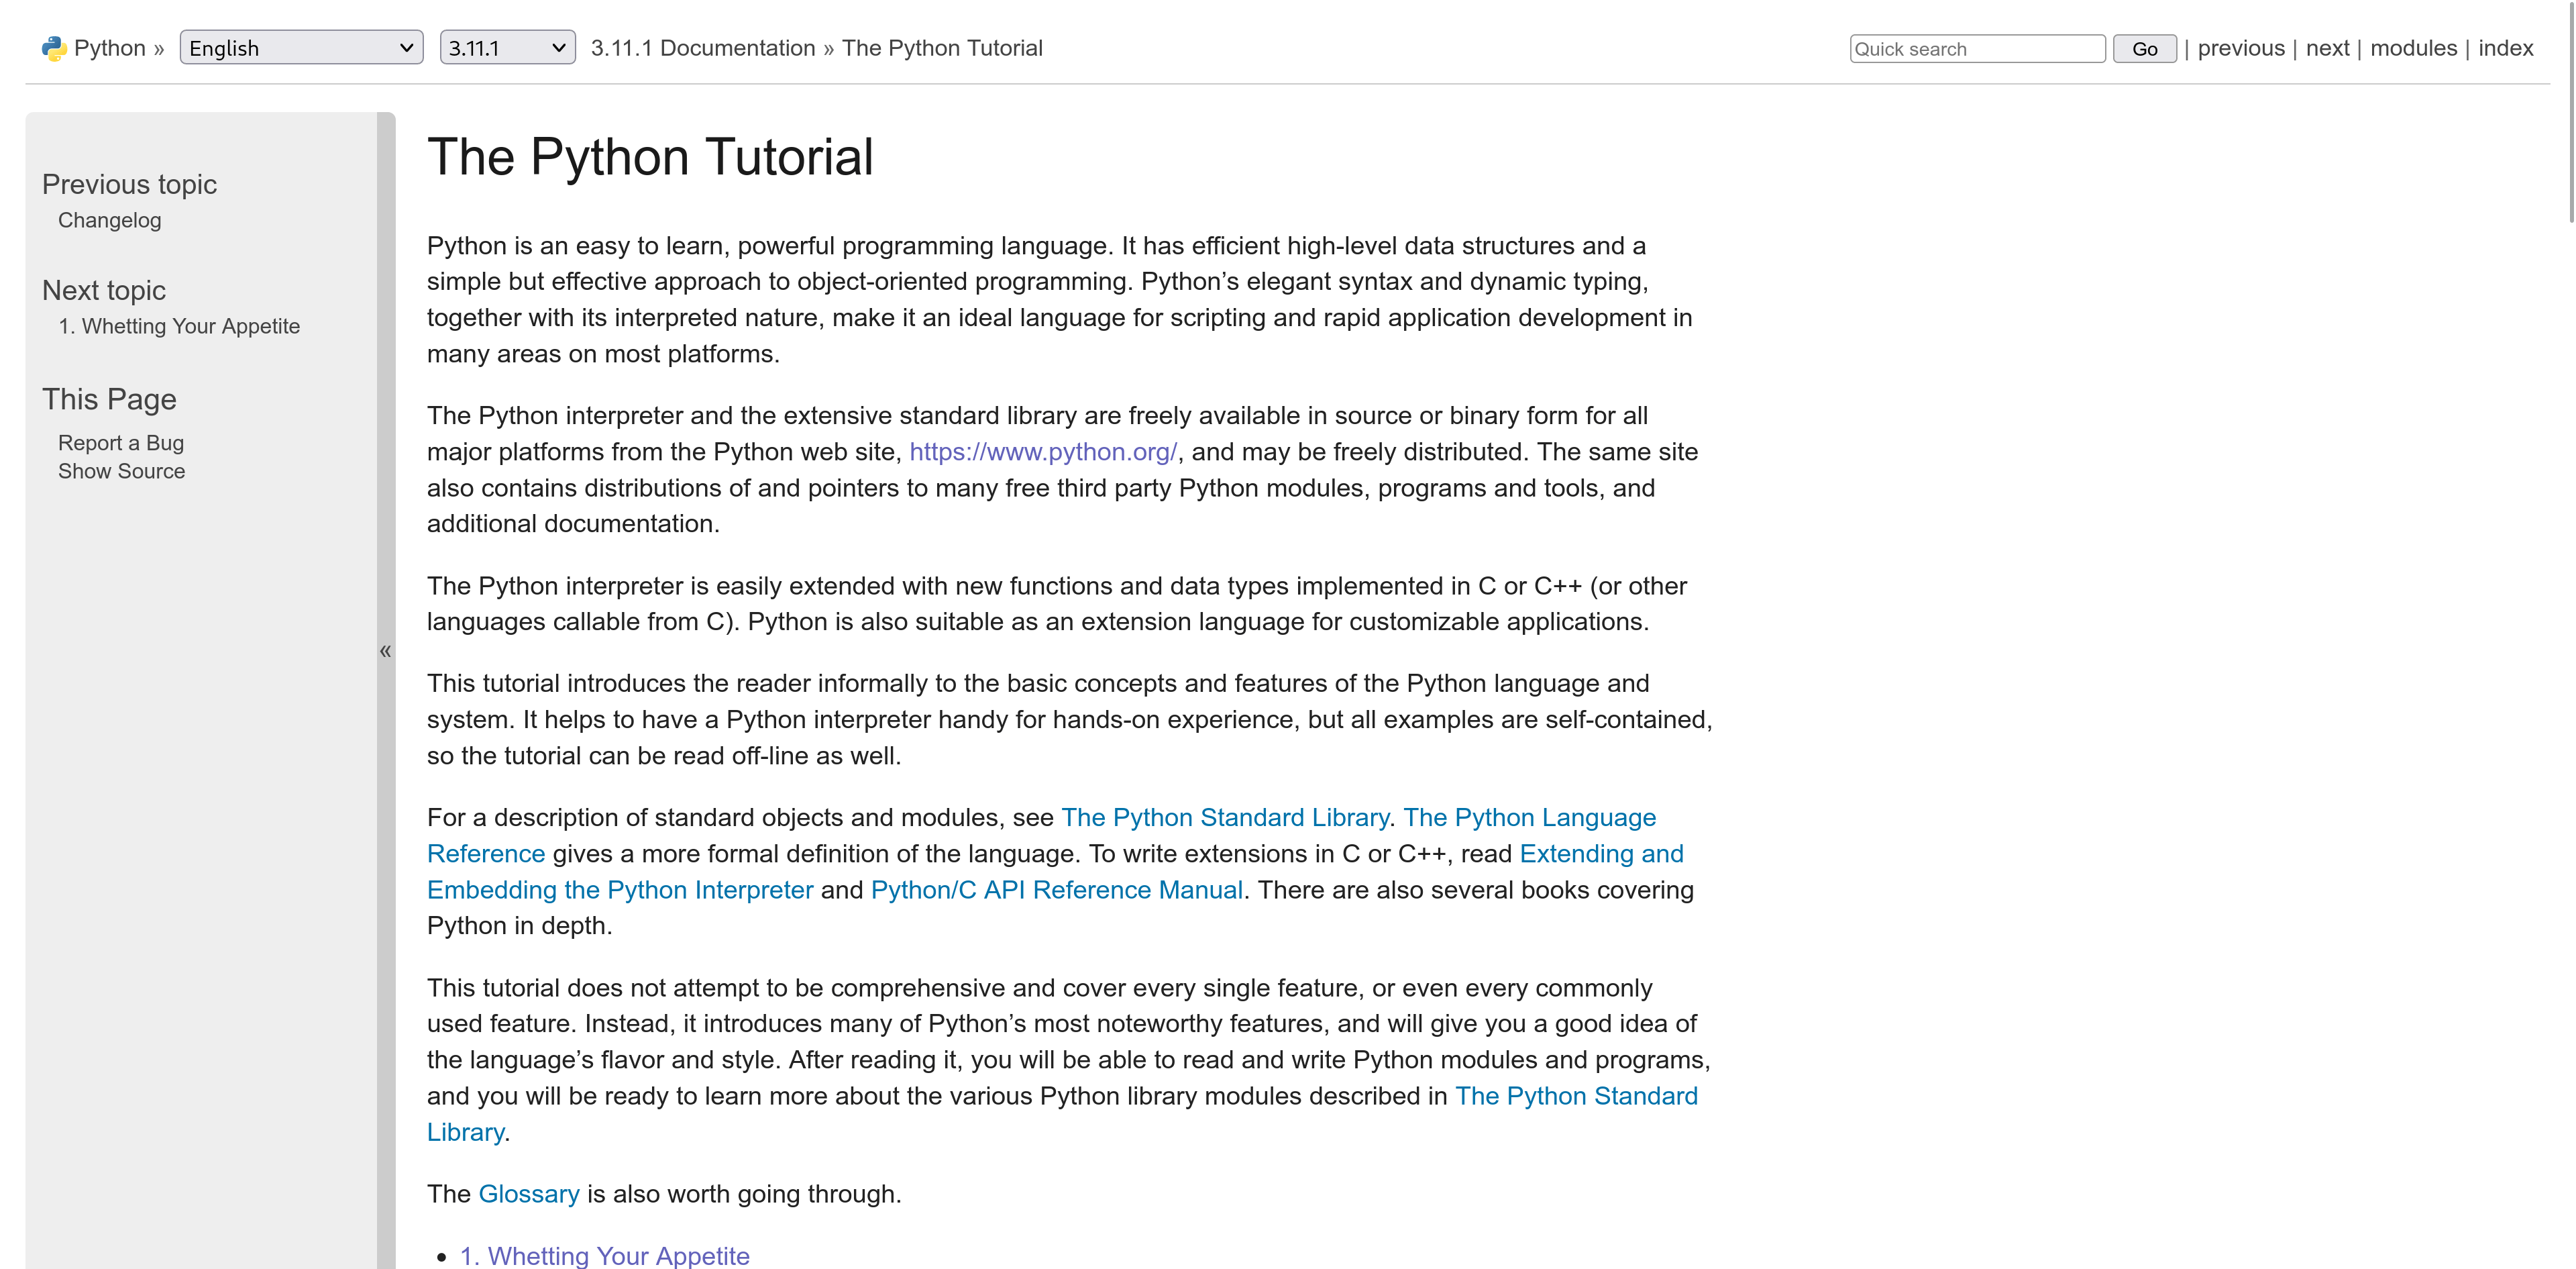
\includegraphics[width=\textwidth]{img/webseite-tuten}}
        \vskip .5em
        \textbf{Englisches Tutorial} \\
        \href{https://docs.python.org/3/tutorial/}{docs.python.org/3/tutorial/}

        \column[T]{.33\textwidth}
        \fbox{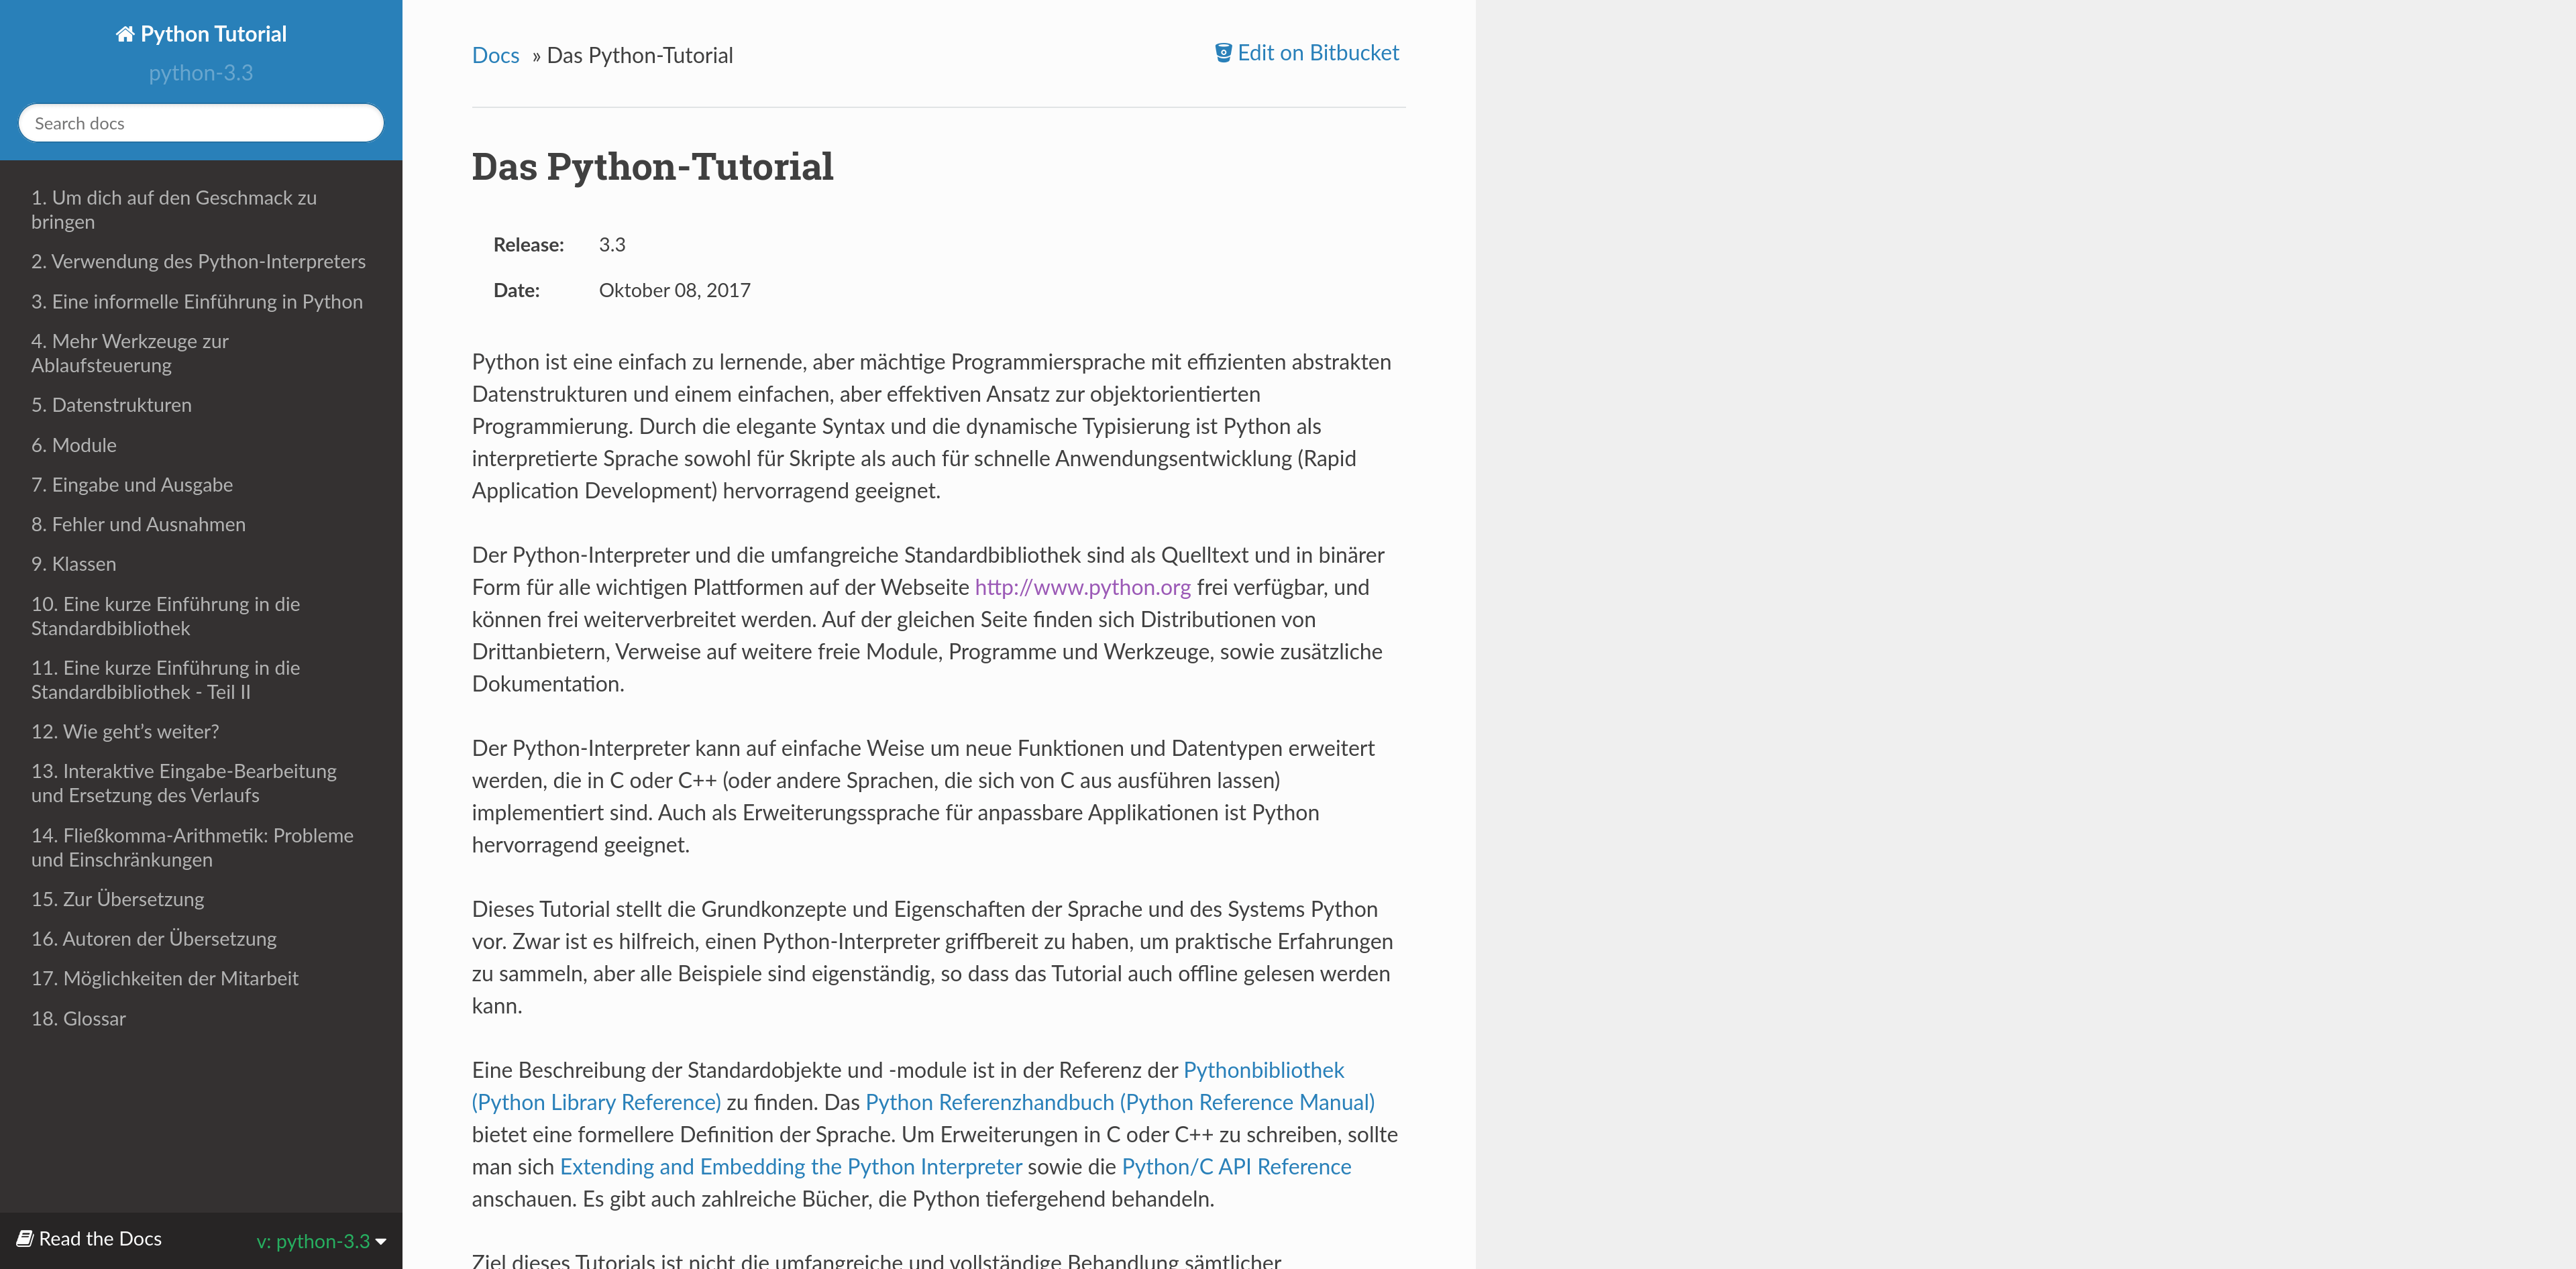
\includegraphics[width=\textwidth]{img/webseite-tutde}}
        \vskip .5em
        \textbf{Deutsches Tutorial} \\
        \href{https://py-tutorial-de.readthedocs.io/}{py-tutorial-de.readthedocs.io}

        \column[T]{.33\textwidth}
        \fbox{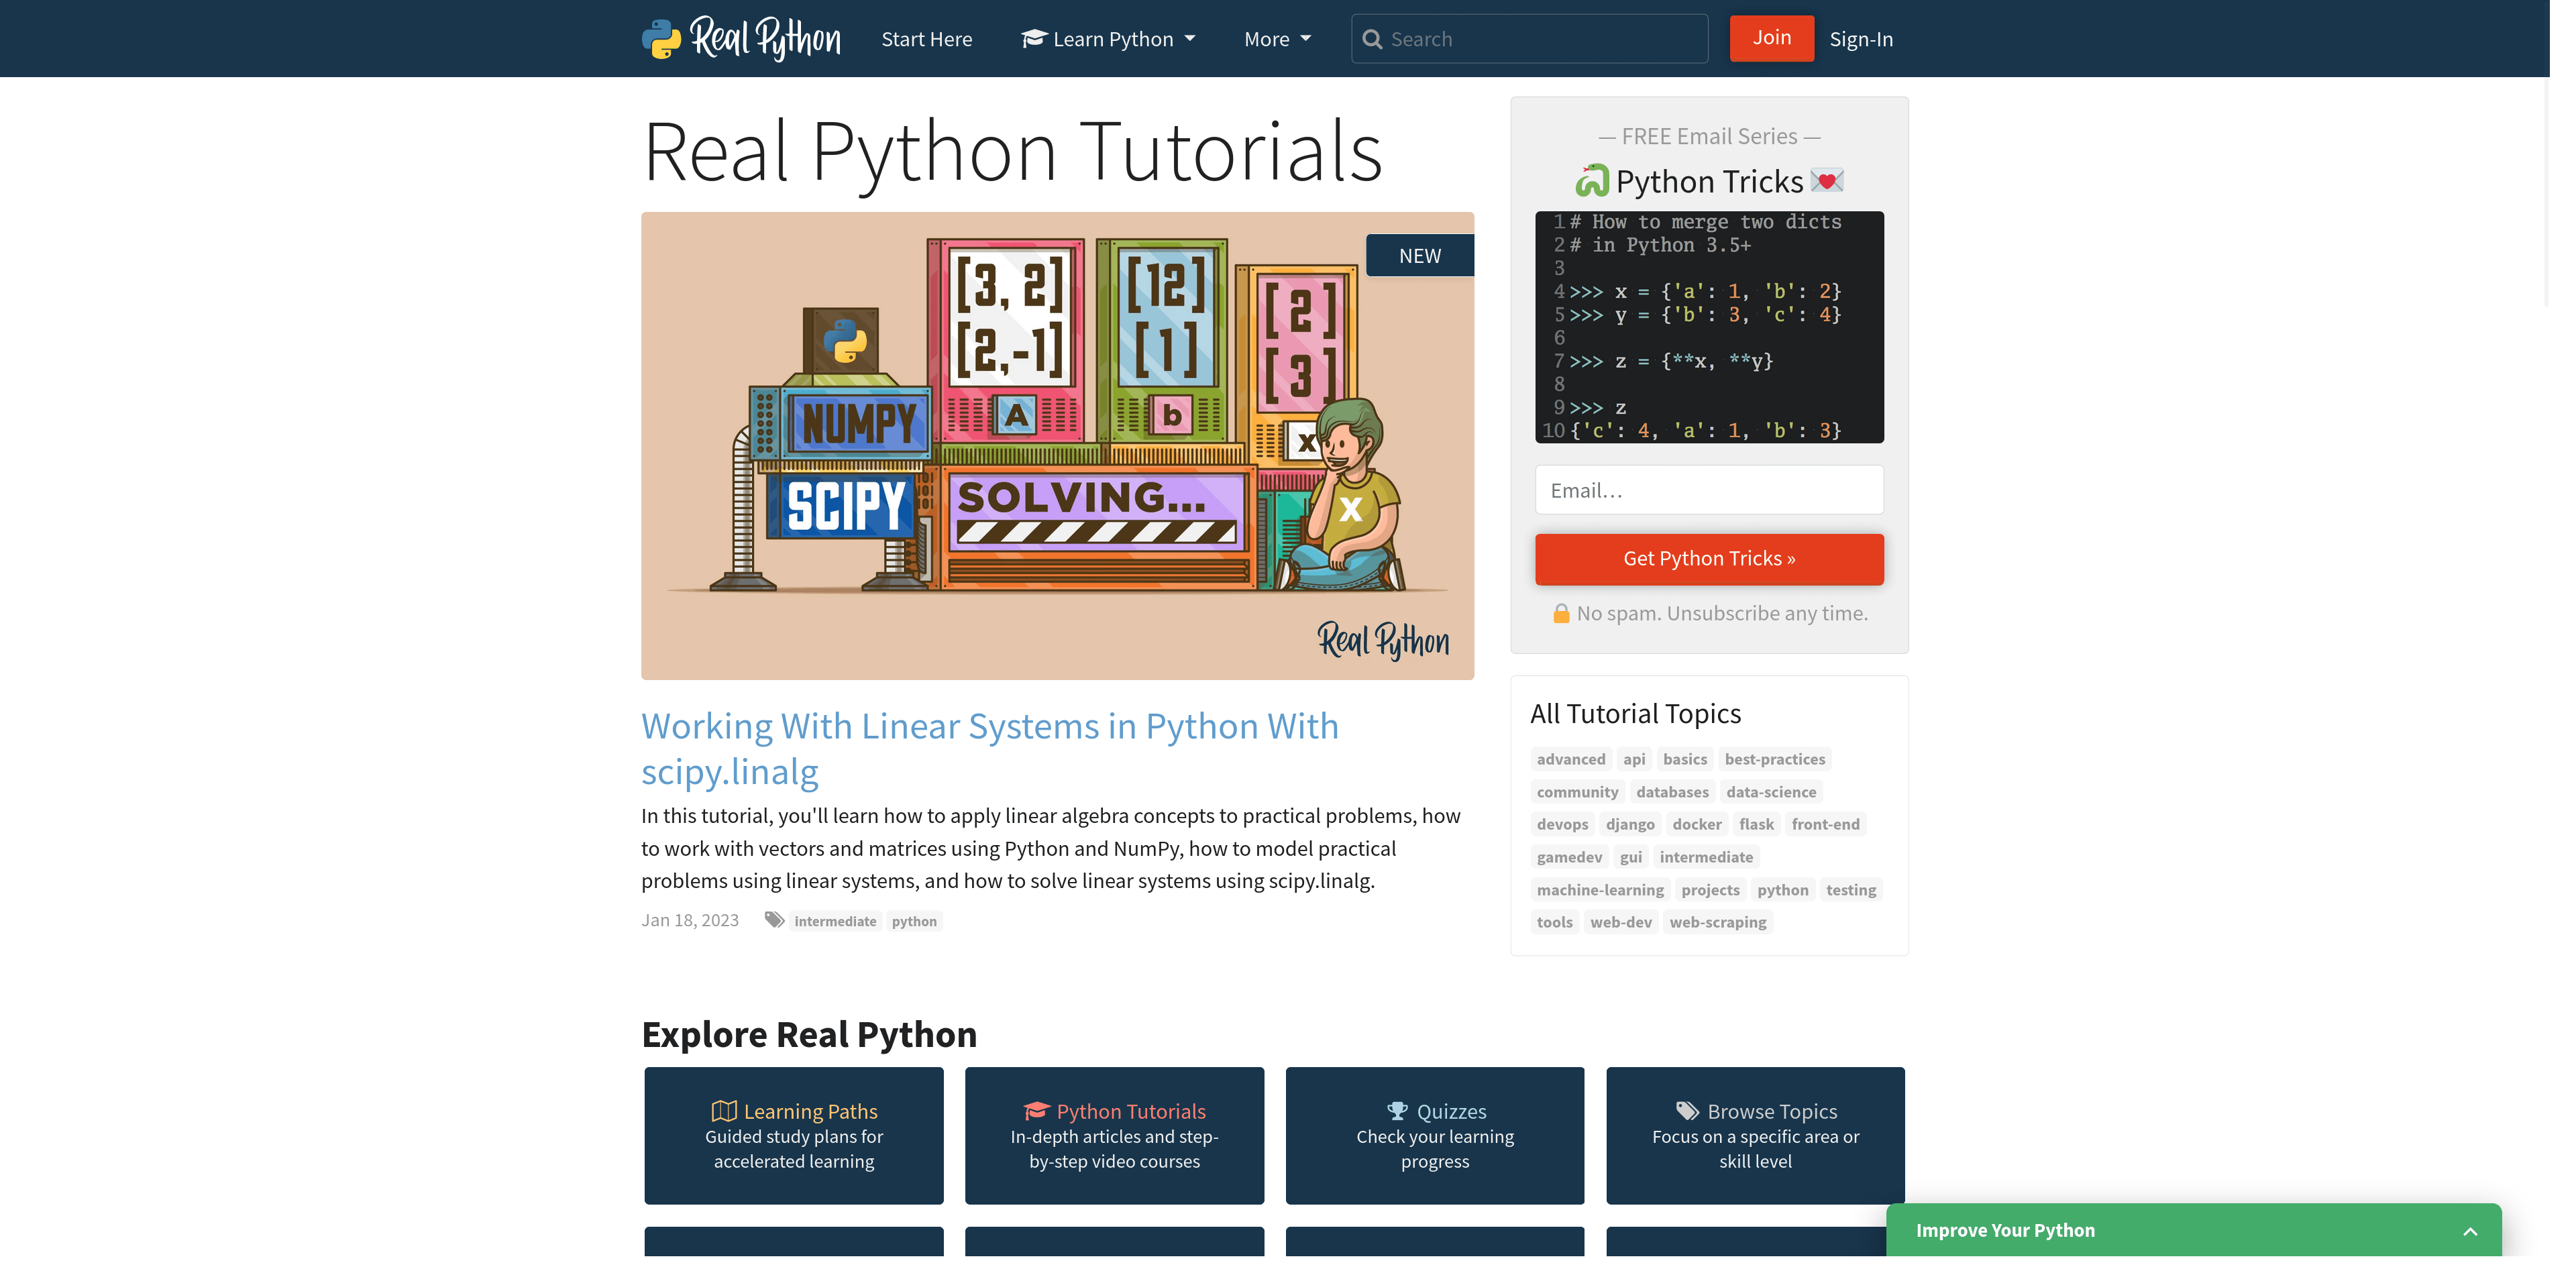
\includegraphics[width=\textwidth]{img/webseite-realpython}}
        \vskip .5em
        \textbf{Real Python} \\
        \href{https://realpython.com/}{realpython.com}
    \end{columns}
\end{frame}
}

%%% Folie
{
\scriptsize

\begin{frame}{Einfache Versuche im Interpreter}
    \begin{columns}
        \column[T]{.7\textwidth}
        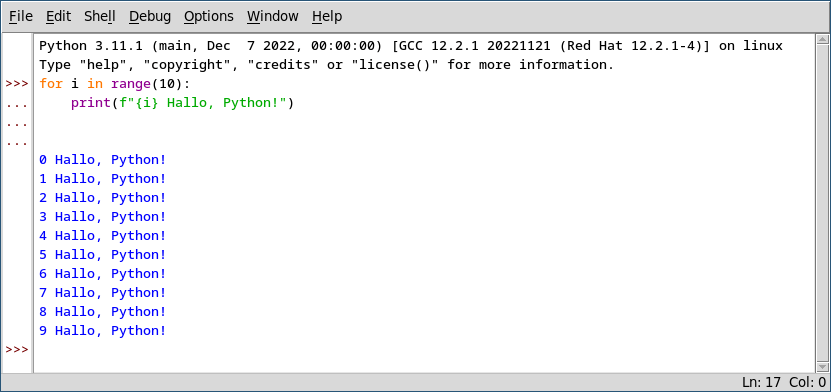
\includegraphics[width=\textwidth]{img/python-interpreter-idle}

        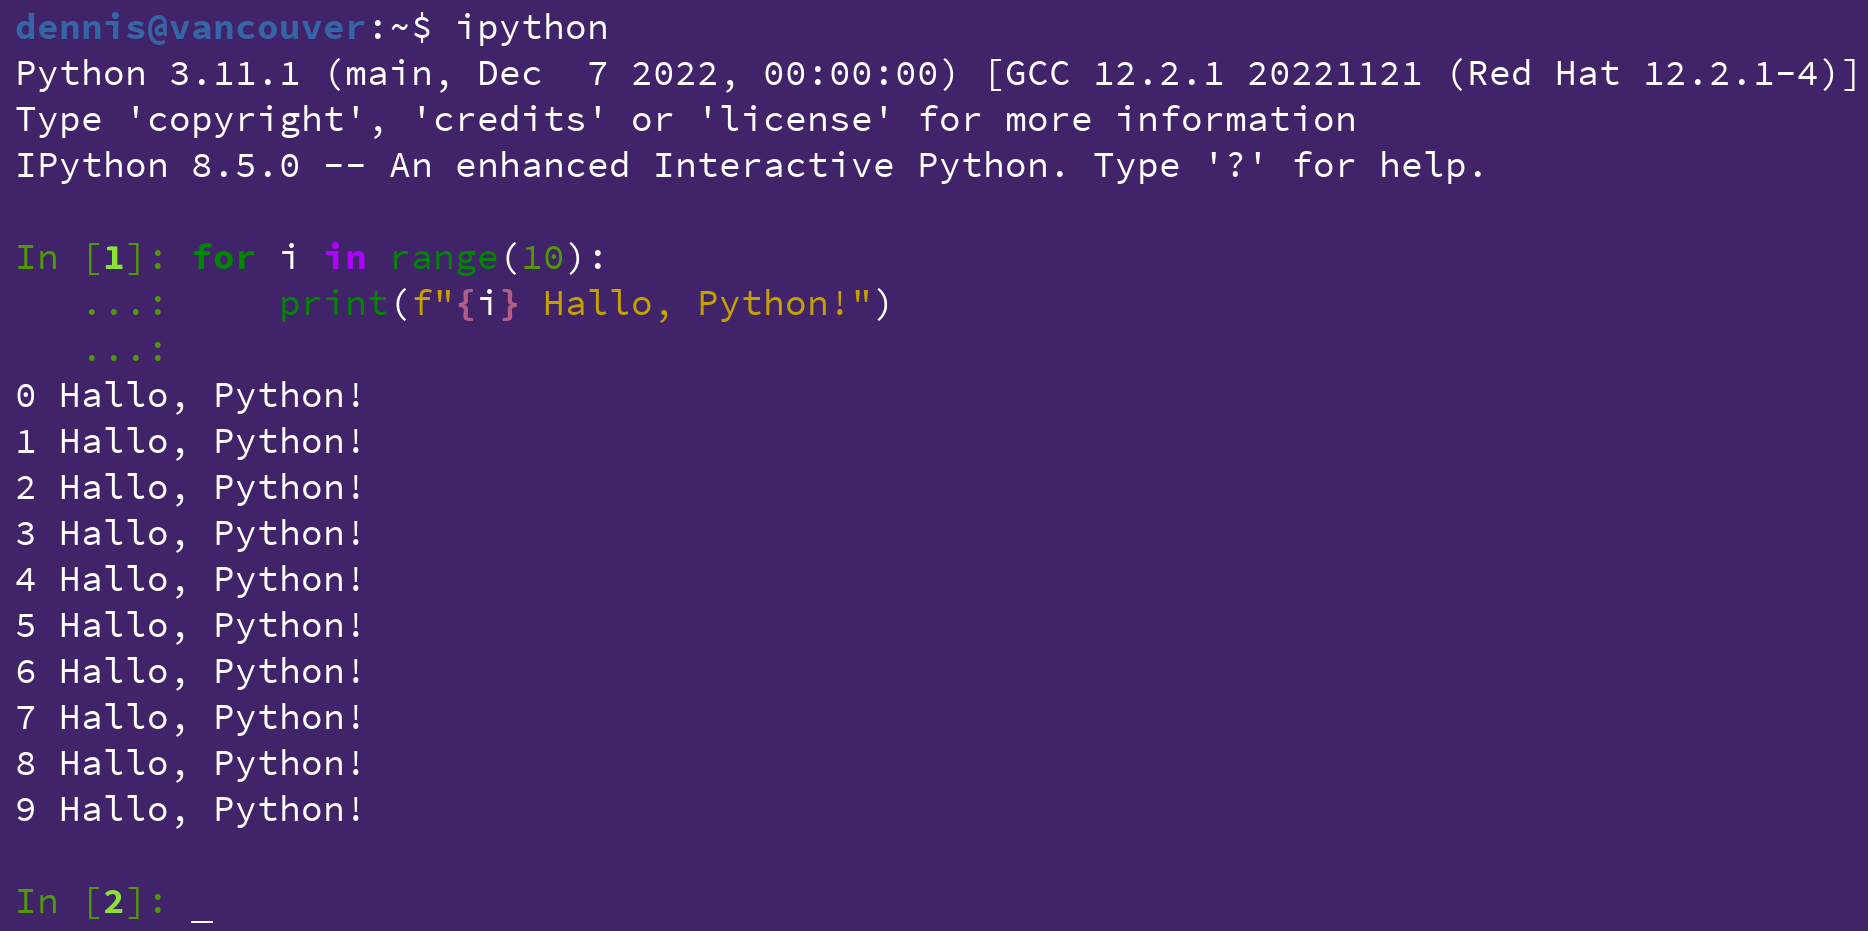
\includegraphics[width=\textwidth]{img/python-interpreter-ipython}

        \column[T]{.3\textwidth}
        \Justified{
            Für einfache Versuche oder kleine Wegwerfskripte bietet Python einen
            einfachen Kommandozeileninterpreter, der jede eingegebene Codezeile
            direkt ausführt und ihr Ergebnis ausgibt. Das Prinzip wird auch REPL
            genannt von \textit{Read, Evaluate, Print, Loop}.
            \smallskip

            Traditionell wird der Interpreter, wie im unteren Bild gezeigt, mit dem
            Befehl \texttt{python} in einem Konsolenfenster gestartet. Wobei hier
            die verbesserte Version \texttt{ipython} (separat zu installieren)
            gezeigt wird.
            \smallskip

            Alternativ kann aber auch die im Lieferumfang von Python enthaltene
            grafische Anwendung IDLE gestartet werden.
        }
    \end{columns}
\end{frame}
}

%%% Folie
{
\scriptsize

\begin{frame}{Aufbau eines typischen Python-Projekts}
    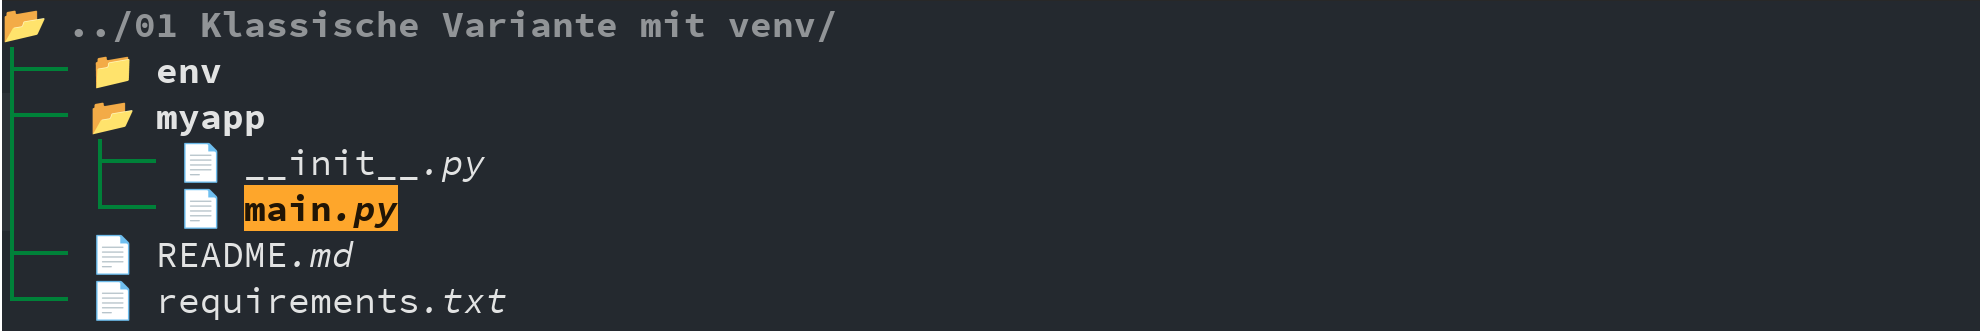
\includegraphics[width=\textwidth]{img/verzeichnisse-venv}
    \smallskip

    \Justified{
        Python schreibt im Grunde genommen keine feste Verzeichnisstruktur für ein
        Projekt vor. Dennoch folgen die meisten Projekte den folgenden Konventionen:
    }

    \begin{itemize}
        \item Im Hauptverzeichnis liegen nur ein README und allgemeine Konfigurationsdateien.
        \item Der eigentliche Quellcode des liegt in einem Unterverzeichnis.
        \item Dieses wird durch eine Datei namens \texttt{\_\_init\_\_.py} als Python-Modul gekennzeichnet.
        \item Weitere Verzeichnisse können Dokumentationen und sonstige Zusatzdaten beinhalten.
        \item Benötigte Zusatzbibliotheken werden in die Datei \texttt{requirements.txt} eingetragen.
        \item Die Installation der Bibliotheken erfolgt in einer virtuellen Python-Umgebung.
    \end{itemize}
\end{frame}
}

%%% Folie
{
\tiny

\begin{frame}[fragile]{Virtuelle Python-Umgebungen verwalten}
    \includegraphics[width=\textwidth]{img/env-aktivieren}

    \Justified{
        \medskip
        Python bot schon früh die Möglichkeit, zusätzliche Codebibliotheken aus dem Internet zu laden
        und auf dem eigenen Rechner zu installieren. Traditionell werden die Bibliotheken allerdings
        systemweit installiert, so dass alle Python-Programme dieselben Bibliotheken nutzen. Da aber
        nicht alle Bibliotheken zusammenpassen oder manche Programm unterschiedliche Versionen einer
        Bibliothek verwenden können, kann dies schnell zu Konflikten führen.
        \medskip

        Python ermöglicht es daher, in einem Unterverzeichnis eine isolierte Python-Umgebung für ein
        einzelnes Projekt zu erstellen. Der exakte Inhalt des Verzeichnisses ist für die praktische
        Nutzung dabei gar nicht relevant. Nur, dass dort die Bibliotheken exakt eines Projekts getrennt von
        den anderen Projekten installiert werden. Folgende Kommandozeilenbefehle werden hierfür benötigt:
        \medskip
    }

    {
    %~ \tiny
    \arrayrulecolor{gray}

    \begin{tabular}{|p{.95\textwidth}|}
        \hline

        \cellcolor{gray!15}
        \texttt{python -m venv env} \\
        \cellcolor{gray!15}
        \textcolor{darkgray}{Neue Pythonumgebung im Verzeichnis \texttt{env} anlegen} \\

        \cellcolor{gray!7}
        \\

        \cellcolor{gray!15}
        \texttt{source env/bin/activate} bzw. \\
        \texttt{. env/bin/activate} \\
        \cellcolor{gray!15}
        \textcolor{darkgray}{\textbf{Linux, Mac:} Python-Umgebung für die laufende Konsolensitzung aktivieren} \\

        \cellcolor{gray!7}
        \\

        \cellcolor{gray!15}
        \texttt{env\textbackslash Scripts\textbackslash activate} \\
        \cellcolor{gray!15}
        \textcolor{darkgray}{\textbf{Windows:} Python-Umgebung für die laufende Konsolensitzung aktivieren} \\

        \cellcolor{gray!7}
        \\

        \cellcolor{gray!15}
        \texttt{deactivate} \\
        \cellcolor{gray!15}
        \textcolor{darkgray}{Aktuelle aktive Python-Umgebung wieder verlassen} \\

        \hline
    \end{tabular}
    }

    \medskip
    \LinkButton{https://realpython.com/python-virtual-environments-a-primer/}{Ausführliche Anleitung}
\end{frame}

%%% Folie
{
\tiny

\begin{frame}[fragile]{Abhängigkeiten installieren mit pip}
    \includegraphics[width=\textwidth]{img/pip-install}

    \includegraphics[width=\textwidth]{img/pip-list}

    \Justified{
        \medskip
        Die Installation und Deinstallation der Bibliotheken erfolgt mit dem Kommandozeilenwerkzeug
        \texttt{pip} durch Ausführen der unten aufgeführten Befehle. Dabei hat es sich als Best-Practice
        etabliert, die Bibliotheken und ihre Versionen in einer Datei namens \texttt{requirements.txt}
        zu beschreiben, damit die Installation jederzeit reproduziert werden kann:
    }

    \begin{lstlisting}[language=Python, gobble=8]
        # Farbige und formatierte Konsolenausgaben
        rich~=13.2
    \end{lstlisting}

    {
    %~ \tiny
    \arrayrulecolor{gray}

    \begin{tabular}{|p{.95\textwidth}|}
        \hline

        \cellcolor{gray!15}
        \texttt{pip install -r requirements.txt} \\
        \cellcolor{gray!15}
        \textcolor{darkgray}{Alle in der angegebenen Datei aufgezählten Bibliotheken installieren} \\

        \cellcolor{gray!7}
        \\

        \cellcolor{gray!15}
        \texttt{pip install \textit{bibliothek}} \\
        \cellcolor{gray!15}
        \textcolor{darkgray}{Manuelle Installation einer einzelnen Bibliothek (nicht empfohlen!)} \\

        \cellcolor{gray!7}
        \\

        \cellcolor{gray!15}
        \texttt{pip uninstall \textit{bibliothek}} \\
        \cellcolor{gray!15}
        \textcolor{darkgray}{Manuelle Deinstallation einer einzelnen Bibliothek (nicht empfohlen!)} \\

        \cellcolor{gray!7}
        \\

        \cellcolor{gray!15}
        \texttt{pip list} \\
        \cellcolor{gray!15}
        \textcolor{darkgray}{Bereits installierte Bibliotheken und ihre Version auflisten} \\

        \hline
    \end{tabular}
    }
\end{frame}
}

%%% Folie
{
\tiny

\begin{frame}[fragile]{Verwendung der Bibliothek und Start der Anwendung}
    \Justified{
        Bei aktivierter virtueller Python-Umgebung kann die Anwendung wie folgt gestartet werden.
        Die hier verwendete Bibliothek \texttt{rich} wurde zuvor dem Projekt hinzugefügt.
    }

    \includegraphics[width=\textwidth]{img/venv-ausfuehren}

    \begin{lstlisting}[language=Python, gobble=8]
        #! /usr/bin/env python
        """
        Minimalbeispiel für ein typisches Python-Projekt.
        """

        import rich
        from rich.prompt import Prompt

        if __name__ == "__main__":
            name = Prompt.ask(
                "[bold bright_magenta]Wie heißt du?[/bold bright_magenta]",
                default="Kain Ame"
            )

            eis = Prompt.ask(
                "[bold bright_magenta]Welches ist dein Lieblingseis?[/bold bright_magenta]",
                choices = ["Schokolade", "Vanille", "Erdbeer"],
                default = "Erdbeer"
            )

            rich.print(f"Hallo, [red]{name}[/red]. Dein Lieblingseis ist [blue]{eis}[/blue]. :red_heart-emoji:\n")
    \end{lstlisting}
\end{frame}
}

%%% Folie
{
\tiny

\begin{frame}{Poetry als moderne Alternative}
    \includegraphics[width=\textwidth]{img/verzeichnisse-poetry}
    \smallskip

    \Justified{
        Für Umsteiger von anderen Programmiersprachen wie zum Beispiel JavaScript/Node.js scheint
        die manuelle Verwaltung virtueller Python-Umgebungen sicher etwas umständlich. In den letzten
        Jahren sind deshalb viele Werkzeuge zur Automatisierung und Vereinfachung wie Poetry erschienen.
        Die Konventionen für die Verzeichnisstruktur sind nahezu dieselben wie bei den älteren Werkzeugen.
        Jedoch entfällt hier das Verzeichnis für die virtuelle Umgebung, da dieses von Poetry automatisch
        außerhalb des Projektverzeichnisses angelegt wird:
    }

    \begin{itemize}
        \item Im Hauptverzeichnis liegen nur ein README und allgemeine Konfigurationsdateien.
        \item Der eigentliche Quellcode des liegt in einem Unterverzeichnis.
        \item Dieses wird durch eine Datei namens \texttt{\_\_init\_\_.py} als Python-Modul gekennzeichnet.
        \item Weitere Verzeichnisse können Dokumentationen und sonstige Zusatzdaten beinhalten.
    \end{itemize}

    \Justified{
        Ebenfalls neu ist die Datei \texttt{pyproject.toml}, welche die \texttt{requirements.txt}
        ersetzt. Sie enthält neben den benötigten Bibliotheken noch weitere Einstellungen für
        das Projekt. Die Datei \texttt{poetry.lock} stellt sicher, das bei einer Wiederholung der
        Installation die exakt gleichen Versionen aller Bibliotheken installiert werden.
        \smallskip
    }

    \LinkButton{https://python-poetry.org/}{Poetry Paketverwaltung}
\end{frame}
}

%%% Folie
{
\tiny

\begin{frame}[fragile]{Wichtige Befehle für Poetry}
    \includegraphics[width=\textwidth]{img/poetry-show}

    \Justified{
        \medskip
        Alle für die Arbeit an einem Projekt relevanten Aufgaben können mit dem \texttt{poetry}
        Kommandozeilenwerkzeug erledigt werden. Eine Unterscheidung, ob eine virtuelle Python-Umgebung
        verwaltet oder Bibliotheken darin installiert werden sollen, gibt es nicht. Peoptry kümmert
        sich im Hintergrund selbstständig darum, eine virtuelle Umgebung für das Projekt anzulegen
        und zu verwalten.
        \medskip
    }

    {
    %~ \tiny
    \arrayrulecolor{gray}

    \begin{tabular}{|p{.95\textwidth}|}
        \hline

        \cellcolor{gray!15}
        \texttt{poetry init} \\
        \cellcolor{gray!15}
        \textcolor{darkgray}{Anlegen eines neuen Python-Projekts} \\

        \cellcolor{gray!7}
        \\

        \cellcolor{gray!15}
        \texttt{poetry install} \\
        \cellcolor{gray!15}
        \textcolor{darkgray}{Erzeugen der Python-Umgebung und Installation aller bekannten Abhängigkeiten} \\

        \cellcolor{gray!7}
        \\

        \cellcolor{gray!15}
        \texttt{poetry add \textit{bibliothek}} \\
        \cellcolor{gray!15}
        \textcolor{darkgray}{Installieren und Hinzufügen einer weiteren Bibliothek zum aktuellen Projekt} \\

        \cellcolor{gray!7}
        \\

        \cellcolor{gray!15}
        \texttt{poetry remove \textit{bibliothek}} \\
        \cellcolor{gray!15}
        \textcolor{darkgray}{Deinstallieren und Entfernen einer Bibliothek aus dem aktuellen Projekt} \\

        \cellcolor{gray!7}
        \\

        \cellcolor{gray!15}
        \texttt{poetry show} \\
        \cellcolor{gray!15}
        \textcolor{darkgray}{Informationen zu allen installierten Bibliotheken anzeigen} \\

        \cellcolor{gray!7}
        \\

        \cellcolor{gray!15}
        \texttt{poetry run \textit{befehl}} \\
        \cellcolor{gray!15}
        \textcolor{darkgray}{Ausführen des übergebenen Kommandozielenbefehls innerhalb der Python-Umgebung} \\

        \cellcolor{gray!7}
        \\

        \cellcolor{gray!15}
        \texttt{poetry shell} \\
        \cellcolor{gray!15}
        \textcolor{darkgray}{Start einer Sub-Shell mit aktivierter, virtueller Pyhton-Umgebung} \\

        \cellcolor{gray!7}
        \\

        \cellcolor{gray!15}
        \texttt{poetry shell} \\
        \cellcolor{gray!15}
        \textcolor{darkgray}{Verlassen der Sub-Shell und somit der virtuellen Python-Umgebung} \\

        \hline
    \end{tabular}
    }
\end{frame}
}

%%% Folie
{
\tiny

\begin{frame}[fragile]{Start eines Poetry-Projekts}
    \includegraphics[width=\textwidth]{img/poetry-run1}

    \includegraphics[width=\textwidth]{img/poetry-run2}

    \Justified{
        \medskip
        Mit dem Kommando \texttt{poetry run \textit{befehl}} lässt sich die virtuelle Python-Umgebung
        temporär für die Ausführung das angegebenen Betriebssystembefehls aktivieren. Meistens wird
        dies einfach nur genutzt, um die Anwendung wie oben gezeigt zu starten. Es kann aber auch eine
        IDE wie Visual Studio Code somit gestartet werden, um ein Debuggen der Anwendung darin zu
        ermöglichen:
    }

    \begin{lstlisting}[language=sh, gobble=8]
        poetry run code
    \end{lstlisting}

    \includegraphics[width=\textwidth]{img/poetry-vscode}
\end{frame}
}

% Code und Screenshot

%-------------------------------------------------------------------------------
\section{Praxisbeispiel: KI-Bildgenerator}
%-------------------------------------------------------------------------------

\begin{frame}{Version 1: Einfaches Skript}
    \textbf{Verzeichnisstruktur}
    \includegraphics[width=\textwidth]{img/ipaint-dateien-version1}

    \textbf{Programmausgabe}
    \includegraphics[width=\textwidth]{img/ipaint-ausgabe-version1}

    \Justified{
        \medskip
        Dies ist die simpelste Version des Beispiels. Es handelt sich um ein ganz
        einfaches Python-Skript, das eine fest einprogrammierte Anfrage an den DALL-E
        Text2Image-Bildgenerator von OpenAI sendet und dann ein Browserfenster mit dem
        erzeugten Bild öffnet. Durch Anpassen des Quellcodes können aber schon ganz interessante
        Ergebnisse erzielt werden.
        \medskip
    }

    \begin{columns}
        \column[T]{.2\textwidth}
        \includegraphics[width=\textwidth]{img/ipaint-generiert1}

        \column[T]{.2\textwidth}
        \includegraphics[width=\textwidth]{img/ipaint-generiert2}

        \column[T]{.2\textwidth}
        \includegraphics[width=\textwidth]{img/ipaint-generiert3}

        \column[T]{.2\textwidth}
        \includegraphics[width=\textwidth]{img/ipaint-generiert4}

        \column[T]{.2\textwidth}
        \includegraphics[width=\textwidth]{img/ipaint-generiert5}
    \end{columns}
\end{frame}

\begin{frame}{Version 2: Klassenbasierte Struktur}
    \textbf{Verzeichnisstruktur}
    \includegraphics[width=\textwidth]{img/ipaint-dateien-version2}

    \textbf{Programmausgabe}
    \includegraphics[width=\textwidth]{img/ipaint-ausgabe-version2}

    \Justified{
        \medskip
        Diese Version unterscheidet sich deutlich von der Vorgängerversion. Anstelle
        des einfachen Skripts tritt eine richtige Python-Anwendung, die mit Klassen
        und Modulen strukturiert wurde:
        \smallskip

        Beispielsweise übernimmt die Klasse \texttt{ApiKeyManager} das Einlesen und
        Bereitstellen der API-Keys. Im Unterpaket \texttt{generator} befinden sich
        hingegen eine allgemeine Schnittstelle für beliebige Text2Image-Bildgeneratoren
        sowie eine konkrete Implementierung anhand von OpenAI DALL-E. Das Hauptprogramm
        muss daher lediglich den Dialog mit dem Anwender umsetzen und dabei die jeweiligen
        Klassen verwenden. Auf dieser Grundlage kann das Programm beliebig weiterentwickelt
        werden. Der Fantasie sind keine Grenzen gesetzt. \smiley{}
    }
\end{frame}

\begin{frame}{Version 3: Grafische Benutzeroberfläche}
    \textbf{Verzeichnisstruktur}
    \includegraphics[width=\textwidth]{img/ipaint-dateien-version3}

    \textbf{Programmausgabe}
    \includegraphics[width=\textwidth]{img/ipaint-ausgabe-version3}

    \Justified{
        \medskip
        Diese Version baut auf der vorherigen Version auf und ersetzt die bisher sehr
        spartanische Benutzerinteraktion durch ein modernes Text User Interface. Der
        meiste Quellcode ist daher identisch. Lediglich die Datei \texttt{main.py} musste
        hierfür neugeschrieben werden, wobei hier wieder die \texttt{textual}-Bibliothek
        zum Einsatz kommt.
    }
\end{frame}

%%%%%%%%%%%%%%%%%%%%%%%%%%%%%%%%%
%%%%% TODO: Weitere Folien %%%%%%
%%%%%%%%%%%%%%%%%%%%%%%%%%%%%%%%%

% Ggf. hier Code-Ausschnitte anhand derer die Sprache Python erklärt werden kann.
% Shebang, Allgemeine Syntax, if __name__ ..., Funktionen definieren und aufrufen,
% Objekte erzeugen, Variablen und Duck Typing, Klassen definieren, ...

%%% Folie
\begin{frame}[allowframebreaks]{ChatGPT über Duck Typing}
    \begin{center}
        \includegraphics[width=.9\textwidth]{img/chatgpt-ducktyping1}
    \end{center}

    %%%
    \framebreak

    \begin{center}
        \includegraphics[width=.9\textwidth]{img/chatgpt-ducktyping2}
    \end{center}

    \begin{center}
        \includegraphics[width=.24\textwidth]{img/duck-typing1}
        \hfill
        \includegraphics[width=.24\textwidth]{img/duck-typing2}
        \hfill
        \includegraphics[width=.24\textwidth]{img/duck-typing3}
        \hfill
        \includegraphics[width=.24\textwidth]{img/duck-typing4}
    \end{center}
\end{frame}

%%%%%%%%%%%%%%%%%%%%%%%%%%%%%%%%%
%%%%% TODO: Weitere Folien %%%%%%
%%%%%%%%%%%%%%%%%%%%%%%%%%%%%%%%%

%%% Folie
\begin{frame}{Ergebnis unseres kleinen Programms}
    %~ \begin{columns}
        %~ \column[T]{.4\textwidth}
        %~ \includegraphics[width=\textwidth]{img/ai-gallery1}

        %~ \column[T]{.4\textwidth}
        %~ \includegraphics[width=\textwidth]{img/ai-gallery2}
    %~ \end{columns}

    %~ \begin{columns}
        %~ \column[T]{.8\textwidth}
        %~ \includegraphics[width=\textwidth]{img/ai-gallery3}
    %~ \end{columns}

    \begin{center}
        \includegraphics[width=\textwidth]{img/ai-gallery}
    \end{center}
\end{frame}
